% thesis.tex
% This is the main file, which calls up preamble.tex, frontmatter.tex, and thesis.bib as needed.

% Frontmatter shortcuts; note the extra space at the end, which is unfortunately necessary:
\newcommand\myname{Marcello Alves de Sales Junior }
\newcommand\mytitle{A Key-Value-based Persistence Model for Sensor Networks} 
\newcommand\thismonth{December } 
\newcommand\thisyear{2009 }

% Shortcuts (add your own...):
\newcommand{\N}{\mathbb{N}}
\newcommand{\Z}{\mathbb{Z}}
\newcommand{\Q}{\mathbb{Q}}
\newcommand{\R}{\mathbb{R}}
\newcommand{\C}{\mathbb{C}}
\newcommand{\doubleS}{\mathbb{S}}
\newcommand{\vnorm}[1]{\left\|#1\right\|}
\newcommand{\degree}{\ensuremath{^\circ}}
\newcommand{\superscript}[1]{\ensuremath{^{\textrm{#1}}}}
\newcommand{\subscript}[1]{\ensuremath{_{\textrm{#1}}}}
% One of the following two has to be commented out:
%% draftpreamble.tex, to be used with thesis.tex
% This contains the TeX definitions for layout, style, etc., useful for the *draft* of your thesis.
% For the final version of your thesis, use preamble.tex

%%%%% TeX class and packages

\documentclass[12pt,oneside]{book}

\usepackage{amsthm,amsmath,amssymb,amsfonts,latexsym,graphicx,enumerate,setspace}
%\usepackage{color}                       % For creating colored text and background
%\usepackage{hyperref}                 % For creating hyperlinks in cross references
% other possibly useful packages: textcomp,mathrsfs,amscd,epsfig,euscript,cancel

%%%%% Layout

\voffset=-.8in 
\oddsidemargin=0in
\evensidemargin=0in
\textwidth=6.5in
\textheight=9in

\pagestyle{plain}

%%%%% Style of theorems, definitions, examples, equations, etc.

\theoremstyle{plain} % Heading is bold, text italic.
\newtheorem{theorem}{Theorem}[chapter]
\newtheorem{lemma}[theorem]{Lemma}
\newtheorem{proposition}[theorem]{Proposition}
\newtheorem{corollary}[theorem]{Corollary}
\newtheorem{conjecture}{Conjecture}[chapter]

\theoremstyle{definition}  % Heading is bold, text is roman
\newtheorem{definition}{Definition}[chapter]
\newtheorem{example}{Example}[chapter]

\theoremstyle{remark}  % Heading is italic, text is roman
\newtheorem*{remark}{Remark}
\newtheorem*{note}{Note}
\newtheorem{claim}{Claim}[chapter]

%%%%% Appendix style

\renewcommand\appendix[1]{
\chapter*{#1}
\addcontentsline{toc}{chapter}{#1}
}

%%%%% Comment command, useful for editing

\newcommand\comment[1]{{\sc Comment:} {\bf #1}}

%%%%% Draft title page

\begin{document}

\thispagestyle{empty}

\[ \]
\vspace{1in}

\begin{center}
{\Large \bf \mytitle}

\vspace{1.5in}

\myname

\vspace{1.5in}

Version of \today

\end{center}

\tableofcontents 
  % eco-friendly draft version
% preamble.tex, to be used with thesis.tex
% This contains the TeX definitions for layout, style, etc., as well as the first few pages of your thesis: title page, copyright page, approval page, abstract, acknowledgments, tables of contents, tables, and figures.
% The layout commands should give the correct margins according to the graduate division's guidelines

%%%%% TeX class and packages

\documentclass[12pt,oneside]{sfsuthesis}
\usepackage{amsthm,amsmath,amssymb,amsfonts,latexsym,graphicx,enumerate,setspace,verbatim,makeidx,subfigure, multirow, url, soul}
\usepackage[subfigure]{tocloft}
\usepackage{color}                       % For creating colored text and background
%\usepackage{hyperref}                 % For creating hyperlinks in cross
%references
% other possibly useful packages: textcomp,mathrsfs,amscd,epsfig,euscript,cancel

%%%%% Layout
% These numbers might depend on your printer. Check the margins and compare them to the Graduate Division's
% guidelines. If there's something off, try playing with the numbers...
%
% For chapters:
%     Must have a minimum of 1.5in margin on left and 1in on all other sides.  Where there are page numbers
%     (whether on top or bottom), must have one additional inch between the page number and the text, for a
%     total of 2in between the edge of the paper and the text.
% For frontmatter pages:
%     The same margin numbers generally work, except for the Title Page, so you will notice that we use
%     some numbers for \textheight and \footskip right here, and then change them below, right after
%     generating the Title Page.

\hoffset=.5in 
\oddsidemargin=0in
\evensidemargin=0in
\topmargin=0.1in 
\headheight=0in
\headsep=1in
\footskip=.8in
\textwidth=5.9in
\textheight=7in

\setcounter{secnumdepth}{3}
\setcounter{tocdepth}{3}

\pagestyle{plain}

\doublespacing

%%%%% Style of theorems, definitions, examples, equations, etc.

\theoremstyle{plain} % Heading is bold, text italic.
\newtheorem{theorem}{Theorem}[chapter]
\newtheorem{lemma}[theorem]{Lemma}
\newtheorem{proposition}[theorem]{Proposition}
\newtheorem{corollary}[theorem]{Corollary}
\newtheorem{conjecture}{Conjecture}[chapter]

\theoremstyle{definition}  % Heading is bold, text is roman
\newtheorem{definition}{Definition}[chapter]
\newtheorem{example}{Example}[chapter]

\theoremstyle{remark}  % Heading is italic, text is roman
\newtheorem*{remark}{Remark}
\newtheorem*{note}{Note}
\newtheorem{claim}{Claim}[chapter]

%%%%% Appendix style

\renewcommand\appendix[1]{
\chapter*{#1}
\addcontentsline{toc}{chapter}{#1}
}

%%%%% Source-Code listings

\usepackage{courier}
\usepackage{color}
\usepackage{xcolor}
\usepackage{listings}

\lstset{commentstyle=\tiny,captionpos=t,tabsize=2,frame=lines,keywordstyle=\color{blue}\tiny,commentstyle=\color{gray}\tiny,stringstyle=\color{red}\tiny,numbers=left,numberstyle=\tiny,breaklines=true,showstringspaces=false,basicstyle=\tiny,emph={label}}

%\definecolor{darkgreen}{named}{green}
%\definecolor{darkblue}{named}{blue}
%\definecolor{darkred}{named}{red}
%\definecolor{grau}{named}{gray}
%\let\Righttorque\relax
%\lstset{
%commentstyle=\itshape\color{darkgreen},
%keywordstyle=\bfseries\color{darkblue},
%stringstyle=\color{darkred},
%extendedchars=true,
%basicstyle=\scriptsize\ttfamily,
%basicstyle=\tiny\ttfamily,
%tabsize=2,
% keywordstyle=\textbf,
%commentstyle=\color{grau},
% stringstyle=\textit,
%numbers=left,
%numberstyle=\tiny,
% für schönen Zeilenumbruch
%breakautoindent = true,
%breakindent = 2em,
%breaklines = true,
%postbreak = ,
%prebreak = \raisebox{-.8ex}[0ex][0ex]{\ensuremath{\lrcorner}},
%prebreak = \raisebox{-.8ex}[0ex][0ex]{\Righttorque},
%showspaces=false, % Keine Leerzeichensymbole
%showtabs=false, % Keine Tabsymbole
%showstringspaces=false,% Leerzeichen in Strings
%}

\usepackage{caption}
\DeclareCaptionFont{white}{\color{white}}
\DeclareCaptionFormat{listing}{\colorbox{gray}{\parbox{\textwidth}{#1#2#3}}}
\captionsetup[lstlisting]{format=listing,labelfont=white,textfont=white}

%% Use fancy chapter headers, with Jos Dingjan's modifications,
%% plus my own tweaks. This style is not part of teTeX,
%% so we are using a local (and renamed) copy.
\usepackage[Lenny]{fncychap}

%Hifens
\usepackage[latin1]{inputenc}
\usepackage[USenglish]{babel}

%Harvard citation style
\usepackage{natbib}
%enhanced items
% http://dante.ctan.org/tex-archive/macros/latex/contrib/enumitem/enumitem.pdf
\usepackage{enumitem}

\begin{document}

\pagenumbering{roman}
\thispagestyle{empty}

\[ \]
\vspace{-1.8in}

\begin{center}
{\mytitle}

\vspace{1.4in}

\singlespace{A thesis presented to the faculty of\\
San Francisco State University\\
In partial fulfillment of\\
The requirements for\\ The degree}

\vspace{.5in}

\singlespace{Master of Science\\ In\\ Computer Science}

\vspace*{\fill}

{by \\[12pt] 
\myname \\[12pt]
San Francisco, California\\[12pt]
\thismonth
\thisyear}
\end{center}

\newpage
\thispagestyle{empty}

$\mbox{}$
\vspace{3in}
\begin{center}
\singlespace{
    Copyright \copyright{} \thisyear by \myname

    \bigskip

    All rights reserved. No part of the material protected by this
    copyright notice may be reproduced or utilized in any form or by any
    means, electronic or mechanical, including photocopying, recording or
    by any information storage and retrieval system, without the prior
    permission of the author.
}
\end{center}

\newpage
\thispagestyle{empty}
\[ \]
\vspace{-1.8in}
\begin{center}
{CERTIFICATION OF APPROVAL}
\end{center}
\vspace{.5in}
\begin{quote}
I certify that I have read {\it \mytitle} by \myname, and that in my opinion
this work meets the criteria for approving a thesis submitted in partial
fulfillment of the requirements for the degree: Master of Science in Computer
Science at San Francisco State University.
\end{quote}

\vspace{1.5in}

\hspace*{\fill}\parbox{3.5in}{
\singlespace{

\hrule{\hspace{3.5in}} \\ 
Prof. Arno Puder, Ph.D.\\
Professor of Computer Science\\
\vspace{1in}
\hrule{\hspace{3.5in}} \\
Prof. Marguerite C. Murphy, Ph.D.\\
Professor of Computer Science

}
}

\newpage
\thispagestyle{empty}
\[ \]
\vspace{-1.8in}
\begin{center}
{\mytitle} \\

\vspace{.5in}

\singlespace{
\myname \\
San Francisco, California \\  
\thisyear \\
}
\end{center}

\vspace{.5in}

%\doublespacing{\noindent
\onehalfspacing{\noindent      
Sensor Networks are becoming more and more important to different science
communities bacause of what they produce: the raw data for different studies.
In order to make use the collected data, researchers may have to dissect the
characteristics of the sensor network in question, regarding different
properties such as the purpose and location of the observed data, as well as
how the data is described. For this reason, this work proposes a set of data
persistence taxonomies based on the state of the art, which can be used to
classify the properties of the produced raw data. In order to evaluate the
proposed taxonomies, this work designs and implements a data persistence
component for NetBEAMS, our case study of modular sensor network infrastructure
developed to improve the operation of the SF-BEAMS environmental sensor
network. In this way, based on empirical analysis regarding proposed
taxonomies for the case study, this work selected mongoDB, a schema-less
document-oriented database instead of the traditional use of relational
databases. As a result based on the experiments conducted, this work suggests
that use of Key-Value Pair datasents in orde tor provide External of
Data-Centric approach. Therefore, the use of a solution of the help decreasing
the complexity related to the data persistence layer for sensor networks with
external or data-centric storage mechanism, and whose purpose is data
archival. Finally, this work proposes different future works such a
data-centric approach using Databa se Shards to store te collected data and Map
Reduce to execute parallel queries over the shards.} \vspace*{\fill}
 
\hspace*{\fill}

\noindent
I certify that the Abstract is a correct representation of the content of this thesis.

\vspace{.5in} 

\hrule{\hspace{3.75in}} \\[-10pt]
Chair, Thesis Committee 
\hspace{2.5in}
Date
\doublespacing
\newpage
\[ \]
\vspace{-1.8in}
\begin{center}{ACKNOWLEDGMENTS}\end{center}

\vspace{.5in}
\begin{quote}
\noindent
Acknowledgments
\end{quote}

\renewcommand{\contentsname}{\vspace{-1.7in} \begin{center} \normalsize \rm TABLE OF CONTENTS \end{center}}
\renewcommand{\listfigurename}{\vspace{-1.7in} \begin{center} \normalsize \rm LIST OF FIGURES \end{center}}
\renewcommand{\listtablename}{\vspace{-1.7in} \begin{center} \normalsize \rm LIST OF TABLES \end{center}}
\renewcommand{\cftchapfont}{\normalfont}
\renewcommand{\cftchappagefont}{\normalfont}
\renewcommand{\cftchapleader}{\cftdotfill{\cftdotsep}} % formatting commands for table of contents
\renewcommand{\cftsecfont}{\normalfont}
\renewcommand{\cftsecpagefont}{\normalfont}
\renewcommand{\cftsecleader}{\cftdotfill{\cftdotsep}}

\newpage \tableofcontents 
\newpage \listoftables % comment out if you don't use tables
\newpage \listoffigures % comment out if you don't use figures

\newpage
\pagestyle{myheadings}
\pagenumbering{arabic} 
\setcounter{page}{1}
   % final version, formatted according to the Graduate
% Division's guidelines

% Main body of work:

%% Configuration of the header strings for the Appendices
%\renewcommand{\chaptermark}[3]{%
%  \markboth{\MakeUppercase{\appendixname\ \thechapter}}%
% {\MakeUppercase{#1}}
%}

% main.tex, to be used with thesis.tex
% This contains the main work of your thesis.


%\bibliography{thesis}  % uses the references stored in Chapter1Radar.bib

\chapter{Introduction}

Sensor networks are commonly used in different areas for different purposes
such as scientific measurements and general population use \cite{sn-intro01}
\cite{sn-intro02}. In the scientific community, they serve as tools to monitor
the state of the environment by storing samples of data in specific periods of
time. For instance, the NASA Jet Propulsion Laboratory uses the Volcano
SensorWeb \cite{sn-ex02}, a sensor network which aims to collect data from
specific volcanoes in Alaska and South Pacific to be used with heuristics
regarding dangerous activities. Similarly, the National Data Buoy Center, a
department of the National Oceanic and Atmospheric Administration (NOAA)
\cite{sn-ex03}, provides online data from different buoys in different coast
shores around the world regarding water quality, tide information, etc, what
characterizes sensor network for environmental monitoring \cite{sn-ex01}.
Therefore, sensor networks can be seen as a very important scientific research
and commercial field with direct application and use of its produced data.

In order to provide access to the collected sensor data, different approaches
can be taken to interrogate sensor devices indirectly by accessing its data in
places called network sink. Similarly, the data model and database system
location may also influence in the process of reusing the collected data. In
this way, the lack of a persistence layer for existing sensor networks requires
a deep understanding about its infrastructure, the nature and location of the
collected data, the chosen data model representation, among others. For
instance, how can a data persistence layer safely represent the collected sensor
devices' properties without the need of restructuring any existing data model?
Should the end users' skills in database system be taken into account or the
use of programming languages to access the data \cite{sn-programming-language}?
This problem is currently faced by the departent of Biology at San
Francisco State University with a marine sensor network managed by
researchers without Computer Science skills. While the data access may impose
the difficulties, technical issues may also rise while the execution of a
sensor network such as growth in terms of number of sensor devices and,
consequently, the number of data produced. Last, but not least, the means to
access the data for reuse is the most important features of the sensor
network, taking into account the different data formats used by the main users
of the system. How can specific collected sensor data be exported to other
formats such as spreadsheets or archived files meant to be shared among
research peers? For these, and many other reasons, the inception of a
persistence storage can be a very challenging problem to solve.

In view of the fact that the persistence storage of a sensor network imposes
many different challenges, this work proposes the review of the current state of
the art for sensor networks in order to provide a data persistence layer for an
existing sensor network. As a matter of fact, this work's first contribution is
the inception of a set of basic taxonomies for data persistence in sensor
networks, proposed to drive an empirical evaluation of different technologies
used in the sensor network community. Furthermore, it also takes a look at
different alternatives not yet explored through experiments for a selected
sensor network as a case study. Similarly, this work makes another novice
contribution by suggesting a ``lighter" data model and database infrastructure
that easily captures sensor network device's observations, taking into account
the non-predictable scalability of its infrastructure, as well as the aspects of
the data's nature such as identity, time and location of the collected data.

This dissertation is organized as follows: the next chapter describes the
literature review as the state of art on sensor networks and data persistence, 
providing the needed foundation for the design of taxonomies in data
persistence for sensor networks in chapter 3. Then, chapter 4 examines the
selected case study and its requirements for a persistence layer, whose
technology properties are evaluated in chapter 5 against the developed
taxonomies. The culmination of this work is chapter 6, which details the design
and implementation of a data persistence solution for the selected case
study. Likewise, chapter 7 discusses the solution by presenting the
measurements and conducted experiments, and describing the findings
and contributions of this work. Last, but not least, chapter 8 presents the
conclusions of this work, together with the possible future works not addressed
here.
% main.tex, to be used with thesis.tex
% This contains the main work of your thesis.

%\bibliography{thesis}  % uses the references stored in Chapter1Radar.bib

\chapter{State of the Art of Data Persistence in Sensor Networks}

In general, this chapter reviews surveys and related papers on sensor networks,
providing a basic introduction about their characteristics to a new audience.
Similarly, it reviews the characteristics of related works that discuss and
provide data persistence solutions for sensor networks, characterizing the
different approaches used to described and model the gathered data from sensor
devices.

%It is important to note that the scope of this literature review is limited to
%our case study described in Chapter 4 and, therefore, it only
%covers a subset of disciplines in sensor networks and data persistence.

\section{Survey in Sensor Networks and Its Infrastructure}

According to \cite{sn-intro02}, sensor networks are specialized types of
network systems comprised of nodes with specific goals such as to produce and
collect data. The former is seen as a sensor device capable of producing data
to the network based on an observation from the environment. On the other
hand, the latter is described as the final destination of the raw data in a
sensor network and called the network data sink, or simply data sink, whose
responsibility is to receive, categorize and store the ``sensed'' data. In
this way, the location of the data sink is determined by the purpose of
the collected data: data nodes are placed in-network close to the sensor
devices when collected data has a life cycle, being discarded after being
utilized. In contrast, data nodes are placed in a centralized node when the
collected data is used for historical purposes.

The following sections describe general properties of sensor networks regarding
infrastructure and components as described in the literature.

\subsection{Properties of Sensor Device Nodes in Sensor Networks}

Each sensor node performs different tasks for the network and, therefore,
influences the method of deployment used. \cite{sn-intro01} identifies that
the deployment of sensor devices can use arbitrary methods such as being
dropped from an airplane, or manually placed at chosen geographic locations.
Moreover, the cited authors also mentioned that the deployment can be done as a
one-time event or as an iterative process, where the sensor devices are moved
to different places as needed.

As noted by \cite{sn-intro01} sensor nodes can be
moved around the deployment location, or remain in one place as a stationary sensor. 
In the case of a sensor network comprised with different
moving sensors, a given sensor node can move occasionally or continuously, as
a result of an accidental side-effect or a desired property of the device. As
a matter of fact, these sensors are automotive or they can be attached to
another moving object. For this reason, \cite{sn-intro01} classifies those
types of mobility as active or passive.

Considering the physical design and capabilities of sensor devices, they range
from microscopic to devices measuring a few cubic feet
\cite{sn-intro02}. In addition to their limited size, their computational
resources and power availability can also be affected, when they are located in
areas of limited access to energy. In this way, \cite{sn-intro01} also
distinguishes how sensor devices are usually designed to either store energy in
batteries or use energy scavenged from solar cells. Even though a sensor
network is designed for a purpose, \cite{sn-intro01} also explains that it can
be comprised of different sensor devices playing different roles in what they
observe in the environment, characterizing the heterogeneity of the sensor
network by the hardware capabilities and what types of data each of them
produce.

Finally, \cite{sn-intro01} mentions that sensor device nodes can communicate
with each other using different media such as radio, diffuse light or
inductive sound, influencing the type of protocols they use to exchange data. They
can have knowledge of their physical location if they are integrated with a
Global Positioning System (GPS) device, which gives the latitude or
longitude coordinate values. Therefore, the cost of these devices may range
from hundreds to thousands of dollars, depending on the design capabilities and functionality of a given device.

\subsection{Properties of the Infrastructure of Sensor Networks}
\label{sec:sn-infrastructure}

The last section discussed the different properties of the sensor devices when
placed in a sensor network. Depending on how they communicate with each other,
\cite{sn-intro02} states that sensor devices can be organized in a
structured, or ad hoc way. For this reason, the infrastructure of sensor
networks differ in topology such as single-hop, star, tree or  graph. Each of
these topologies may influence how the produced data from sensor nodes is
collected and routed to their related data sink. While there are only two
levels of node connectivity in sensor networks deployed as single-hop and
star topologies, sensor networks whose topology is either tree or graph use
multi-hop communication among each of their nodes for data communication from
the devices to the data sink.

The property of coverage on a sensor network is defined by
\cite{sn-intro01} as the physical space ``visible" to the sensors devices, which
is also directly related to the purpose of the network, its size in terms of
the number of nodes deployed and the sensor network lifetime. Therefore,
sensors are deployed in sparse or dense manners, according to the
specification of what needs to be covered by the sensor devices. Furthermore,
considering that some types of sensor devices are very likely to experience regular
hardware failures, \cite{sn-intro02} described sensor network examples with 
redundant nodes that provide better data coverage.
Finally, the coverage of sensor devices also has influence on the connectivity
property of the sensor nodes. In order to communicate with redundant nodes, a
physical connection must exist at all times. On the other hand, lower
level of coverage is related to sporadic communication among the sensor nodes.

The sensor network size is related to the degree of coverage mentioned earlier,
and it is measured by the number of devices deployed. \cite{sn-intro01}
reports examples of sensor networks composed by different ranges of deployed
sensor devices such as dozens, hundreds or even thousands of nodes. However,
the lifetime of a sensor network determines how long these devices are going
to be used, as well as how long the sensor network may exist. For example, an
environmental sensor network \cite{sn-ex01} with the purpose of collecting data
for historic purposes may have their sensor devices continuously performing
their data collection tasks. On the other hand, the lifetime of a
sensor network designed to achieve a specific goal will not exist after the sensor
devices finish their tasks. Finally, \cite{sn-intro02} argues that the
performance related to the orchestration of sensor devices in sensor networks
is related to the constraints defined for quality of service (QoS).  This includes
real-time data delivery within a threshold or for robustness such as
maintaining live data even though a communication link is not available.

All things considered, sensor nodes play a vital role during the execution
of a sensor network, whose infrastructure is characterized by how and where the
sensor nodes are deployed and communicate with each other. The next
section covers the approaches dealing with the problem of this type of system
network.

\section{Persistence Storage for Sensor Networks}
\label{sec:sn-persitence-storage}

As outlined in the last few sections, sensor networks are comprised of
different types of sensor nodes. An important sensor node type is the
data sink because it is where the raw data produced by sensor
nodes resides. Data collection and access in sensor networks is directly
related to the characteristics of the sensor network, its routing mechanisms
and where the data sink is placed within the network.

The type of query mechanism used to directly or indirectly interrogate sensor
devices in a sensor network is directly related to the aforementioned locations
of the collected data. The in-network query processing is used when the
location of the collected data is a local storage site \cite{sn-storage01,
sn-data-centric-storage} within the network; a strategy typically used to maximize the
sensor's resources, while minimizing energy consumption \cite{sn-storage04}. On
the contrary, the a typical centralized query processing is used to search for
values over the collected data when the location is a centralized data
node \cite{sn-storage02}.

When it comes to the data representation, the relational data model
\cite{relational-model} is one of the most traditional approaches used to
describe the collected data of sensor networks, as it is reported in database
systems such as the TinyDB \cite{sn-db-tinydb}. For instance, \cite{sn-db-newop}
proposes a modified version of the SQL language of TinyDB proposed to solve
SQL Join problems, so that the query processing takes into account the location
of the distributed data. Conversely, \cite{sn-provenance} proposes the use of
Data Provenance as the primary guidelines used to describe collected  raw data from
sensor devices.

The following sections describe general properties of sensor networks regarding
data persistence, as reviewed in the literature.

\subsection{Data Use and Where Data is Stored}
\label{sec:sn-data-purpose}
\label{sec:sn-storage-locations}

As presented in the previous section, the raw data is the one in-transit from
the sensor to the storage device, where it is labeled to be
identifiable. It is also referred to as the collected data. 
Initially, the raw data serves as the main outcome of the sensor network.
\cite{sn-provenance} differentiates the use of \textbf{real-time data stream}, when they are generated from a sensor
device whenever the data is requested. In this way, the data is still in its raw
format specified by the sensor manufacturer. However, it is not retained. 
In contrast, the authors describe the data as \textbf{archivable}, when they a
have historical significance and will be processed to be reused by other systems at
a latter time. While the real-time data streams are used and potentially
discarded, the archivable data is stored into secondary memory such as a
hard-disk.

After producing the ``sensed'' values for the observed parameters from the
environment, the sensor node is responsible for sending the raw data to a specific
data node defined by the network infrastructure, as delineated in Section
\ref{sec:sn-infrastructure}. Thus, \cite{sn-data-centric-storage}
describes that the destination for the collected sensor data will be one of two
different types of storage devices: the \textbf{external storage} and the
\textbf{local storage}. In the former type, the sensor sends the
produced data to another sensor node that contains an external storage device.
In the latter the data is stored only within the memory of the device before its 
reading as a real-time data stream. On the whole, the sensor network
infrastructure dictates where the movement performed by the sensor data,
for example, \cite{sn-storage02} sees a wireless sensor networks as a many-to-one data
collection pattern, when its organization is based on single-hop or star. On
the other hand, data may also flow from one intermediate sensor node to another
until it reaches its final data sink when the data organization is structured
as a graph, tree \cite{sn-storage01, sn-data-centric-storage}.

Lastly, the use of different external storage devices can be used
to partition the collected data. This practice is called \textbf{Data-Centric
Storage}, and aims at clustering the collected data from different sensor
devices based on a given a property of the data such as location or time of
creation.

\subsection{Query Processing in Sensor Networks}
\label{sec:query-process}

The query processing in sensor networks is a direct or indirect method of
accessing the collected data stored at data nodes, whose location is determined
by different facts described in the previous section. \cite{sn-data-centric-storage}
describes an example of an \textbf{in-network query processing} when sensor
nodes, acting as data nodes, provides real-time data stream as a response
to queries requesting the device's collected data. Likewise, if the collected
data is in use for a specific period of time, the data is cached in an external
storage device in a close-by data node. In this way, when a query is issued to
the sensor network with these characteristics, the query processor considers 
all data nodes before it returns its final response to the query. In comparison, a sensor
network whose topology is in the form of a star, the data sink is usually
located in the center of the structure, and thus, receives all
the collected data from other sensor devices within the network. For this reason, it 
can be seen as a \textbf{centralized query processing}. Factoring in that a centralized data
sink receives all the collected data from the peer nodes, this query processing
strategy is responsible for responding to indirect queries about the
produced data from the network. 

Based on the literature review, there are advantages and disadvantages related to
each of the query processing approaches described with regards to the
infrastructure of the sensor network. \cite{sn-data-centric-storage} argues that the 
primary purpose of the in-network query processing is to minimize the amount
of data transmitted from sensor devices to a data sink, as sensor devices are
generally limited by energy use. Considering that sensor devices are also used
as data nodes, \cite{sn-storage04} states that this approach can potentially
flood all sensor nodes in the network, thereby decreasing its performance.
For this reason, \cite{sn-storage01} reports the use of the data-centric
storage by organizing the collected data based on its particular property
values. In this way, the query processor hits specific data nodes that contain
the types of data in the range of the requested data concluding that this approach 
decreases the network congestion and maximizes the
capacity on the sensor devices and the performance of the sensor network.

Unlike the in-network, the centralized query processing is related to a regular
database system, located in one of the network nodes. For this reason, this
indirect type of query processing is used when the data purpose of the data is for 
data storage. As a consequence, \cite{sn-storage02} shows that the result of
a many-to-one communication between the centralized data sink
and the other data nodes, this query process does not affect any of the sensor
nodes in the network and, thus, maximizes the sensor device utilization. 
Moreover, this strategy better exposes the collected data to the primary users
raw data, which follows the process of data processing, compression,
aggregation, and so on \cite{sn-db-modeling02}.

Although the approach of centralized query processing maximizes the sensor
nodes capacity and minimize energy consumption, \cite{sn-storage02} explains
that this trade off imposes the creation of the unavoidable development of a
point of traffic concentration or the phenomenon of network congestion. For
this reason, \cite{sn-storage04} describes that different techniques used in 
distributed systems such as the use of master-slave data replication
\cite{sn-data-center-replication-load-balance} or database partitioning
\cite{db-partitioning-relational} can be used to reduce or mitigate the
effects of this funneling.

\section{Data Models and Query Engines for Sensor Networks}
\label{sec:data-models}

Different approaches are used to represent the collected data from sensors.
Some research groups lacking database experience arbitrarily assign data 
descriptors, while others use database technology in a more pragmatic approach.
\cite{sn-programming-language} describes several applications using
various types of languages for accessing the data designed in different data
models. \cite{sn-provenance} reports on the use of a \textbf{Tabular Data Model}
\cite{tabular-model} using comma-separated values (CSV) to organize the
measurements collected from sensor devices. In addition, \cite{sn-db-tinydb} 
describes the use of the \textbf{Relational Data Model} \cite{relational-model} 
as used in the majority of the projects that involves data persistence due to its
popularity in areas such as Software Engineering and Distributed Systems. Finally,
\cite{sn-xml-usage01, sn-xml-usage02} discusses examples of sensor network 
applications that make use of XML \cite{xml} to represent the collected data on a 
\textbf{Structured Data Model}.

The following sections describe the application of each of aforenamed data
models in the context of sensor networks.

\subsection{Tabular Data Model and Query}

The most basic computer application to process data is through the use of
spreadsheets, where data is organized into cells \cite{tabular-model}. When
exported to the so-called comma-separated values (CSV) file format, the
resulting file is comprised of lines of ASCII characters, separated by a
delimiter. The first line represents a header, with the identification of
columns of specific data, where the following lines contain the values
related to each top column. \cite{sn-provenance} reports that the tabular
data model is commonly used to provide data persistence for sensor networks.
The SF-BEAMS environmental sensor networks \cite{sfbeams2006} uses this
approach to distribute the collected data over the Internet using the OPenDAP
\cite{opendap} data format.

This data model can be used in different contexts, as \cite{sn-provenance}
describes that the versions of the same document can be easily managed and
shared among research colleagues using a version-control system such as
Subversion \cite{subversion}.

\subsection{Relational Data Model and its Query Mechanism}

\cite{sn-db-newop} shows the use of the Relational Data Model
\cite{relational-model} as it is used in sensor networks to describe the
collected data from sensor devices. The project described
by the authors is based on the TinyDB database system \cite{sn-db-tinydb}, a
database system specifically built for data nodes of sensor networks. It uses
the same properties and constraints of regular database systems, where the
entities of the sensor network are required to be modeled and represented by
tables.

In order to query the data collected from sensor devices, the use of the 
Structured Query Language (SQL) \cite{sql} is the main language used to extract
the data managed by the system. As mentioned earlier, the default versions of
this language have been modified to give support to the constraints of the
location of the database such as the addition of new SQL operators for TinyDB
\cite{sn-db-newop}.

\subsection{Structured Data Model and its Query Mechanism}

XML is an increasing popular data format used widely by the applications developed
for the Internet. \cite{sn-xml-usage01} reports an efficient way to represent
the collected data from sensors using XML, while the authors of
\cite{sn-xml-usage02} describe a sensor network using XML for data model
representation. In general, the collected data is structured into classes of
relating elements and validated by an XML Schema \cite{xml-schema}.

In order to extract data from XML-based databases, the XML XPath language
\cite{xml-xpath} is often used to query XML data. However, with the inception
of hybrid XML-relational database, \cite{sn-xml-usage03} reported the use XML
as the data model and the use of SQL to query the stored data on the IBM's DB2
database system. 

Other examples of the use of the structured data model using XML is found in
the use of middleware, as the authors of \cite{sn-xml-query-engines} reports.
Such an approach is used for data exchange by the implementing of a middleware
capable of query and extract the collected data from sensor devices
\cite{sn-xml-middleware}. A practical example of the use of XML as a middleware
to communicate between nodes is the communication mechanism used by NetBEAMS
\cite{netbeams2009}. See section the documentation at
\cite{netbeams-dsp-architecture} for details.

\section{Description of the Collected Data}
\label{sec:sn-data-description}

As described in the previous section, the collected data from sensor networks
can be represented by different data models, requiring the knowledge of the
properties of the data. Not to mention that the low-level or raw data produced
by a given sensor device might not include vital details regarding the
origin and identity of the collected data. For this reason, the collected data
is reported to be described in different ways such as Data Provenance or
Annotations.

\cite{sn-provenance} describes Data Provenance as a technique used to describe
those essential properties of the collected data from sensors. One typical
example of the application of Data Provenance is the so-called black-box of an
aircraft, which carries the collection of spatial-temporal data structures
collected from a group of sensors placed in different locations of an
aircraft, as shown by \cite{sn-exemple-blackbox}. Finally, the author describes 
the collected data as used in the process of data recovery and analysis in order to
identify the probable reason of an aircraft accident, by analyzing the time, 
location of the aircraft, and other independent variables from the sensors.

In general, sensor devices produce and preserve data onto their local
storage or transmit them to data nodes as described earlier in this chapter. It
is vital to understand that the majority of these devices output the raw data
in streams of values with any type of delimitation between each other. For
this reason, the process of parsing and labeling each of the values located
in the data stream regularly requires the use of the device's specification
documentation. Similarly, in order to have access to each of the properties of
collected data by a given property related to time or space,
\cite{sn-provenance} also mentions that Metadata\footnote{Data about data}
should be included together with the collected data.

An example of a Data Provenance application is the use of the aggregation of data
over time to estimate the changing effects of the weather in a given region.
For this reason, the collected data from sensor devices need meaningful
annotations to better describe the identity of the collected data, as 
\cite{sn-provenance} reports. Pertinent questions regarding the
data can be asked such as \textbf{what was collected?}, \textbf{When was the
data collected?} or \textbf{Where was the data collected?}. Similarly, while
Data Provenance provides basic mechanisms to describe sensor networks data in
general, others see the importance of the time and position of sensor networks.
\cite{sn-time-series} describes strategies used to cluster distributed sensor
data as time series of data, as well as to decrease the size of data streams
being transmitted in real-time sensor networks when these collected data do
not need to be transferred \cite{sn-data-reduction}.

A different way to describe sensor devices is through the use of
Annotations. \cite{sn-annotation} shows the use of tags to describe data
collected from a physical area monitoring. The sensor network was
designed to monitor moving objects, capturing their location while in
movement and their visual appearance using a video camera. In this way,
adding tags to particular video frames can describe each of them, and
therefore, providing an efficient way to search for a specific frame based on
its visual observations. Similarly, the above referenced project also uses data
provenance to describe its collected data, since each of the collected data 
contains the related GPS coordinates of the observed object.

Finally, data provenance provides practical use of the collected data from
different sensor devices and different sensor networks in the process called
Information Fusison \cite{sn-info-fusion}. \cite{sn-geo-metadata} is an example of
the aggregation of different data from different devices located in different 
geographic sensor networks which is capable of processing spatial-temporal 
queries of real-time or historical data. The following sections describe each 
of the metadata properties as defined by \cite{sn-provenance}, giving different
examples of each of them.

\subsection{Data as an object}

Different sensor devices produce different sets of attributes based on their
capabilities and design. In general, these data sets do not have distinct
names, which lead to difficulties when indices over the properties of the
collected data are required to make them searchable. Specially for the purpose
of data archival, the collected data needs to be identified, giving a meaning
of independence on its own, the same idea behind the unique identification of
entities on the relational data model \cite{relational-model}. Equally,
\cite{sn-provenance} describes that traditional sensor networks use the
collected data for analysis long after the attributes have been collected,
usually before it is categorized and indexed. Annotations and tags are also
names given by \cite{sn-provenance} as means to describe collected sensor data.

Briefly, the collected data is described by the name of the observation
property. For instance, \textbf{temperature} = 73.45 expresses the value of the
observation of the temperature. In other words, the string ``temperature'' is
the property describing the raw collected data 73.45. On the other hand,
the example \textbf{temperature-unit} = ``Fahrenheit" describes the metadata
regarding the temperature.

\subsection{Time of Data Creation}

In order to use the collected data for the purpose of historical analysis, the
use of a point in time is the most prominent feature of the data. Also referred to
as spatial-temporal data, it is considered a pivotal metadata used in different
types of sensor networks such as an aircraft the black-box
\cite{sn-exemple-blackbox}, environmental sensor network \cite{sfbeams2006},
and data communications management systems \cite{sn-dataware-house}. In this
way, Other projects classify data in time-series \cite{sn-time-series-example},
where data is related to all the observations a given sensor device performed
over a period of time. The apparent implications is that all the produced data
is necessary, but \cite{sn-time-series} argued that some sorts of sensor
networks could decrease the creation of ``noisy data sets" based on the proper
clustering of similar time-series data before they are sent to the data
sink.

Based on the guidelines defined by \cite{db-temporal}, the time properties of
the collected data can be divided into two different dimensions: \textbf{valid
time} and the \textbf{transaction time}. The former depicts the point in time
when the observation took place with respect to the real-world space. An
important aspect of this metadata is that since it captures the time when the
observation occurred, its value cannot be changed during its existence, as well
as placing restrictions on the update operations of this constant. Similarly,
the latter type of is the point in time at which a given fact was transferred
to the persistence layer. Either types of time can be used depending on the
requirements of the sensor network. For instance, \cite{sn-dataware-house}
reports that all the data stored by its sensor network uses the time of
collection, but do not use the transaction time for that purpose. Similarly,
\cite{sn-provenance} shows a practical examples of critical queries performed
over the transaction time, when doctors need all the collected data regarding
the heart beat rate from the moment the patient entered the ambulance until
the moment of arrival at the hospital.

When both temporal dimensions are applied, the collected data is referred to as
Bitemporal \cite{db-temporal}. Usually, the data type of this metadata is a
regular timestamps, with any supported precision. To clarify, users may be
interested not only when the temperature of 70 degrees happened, but also when
it was collected to the data sink. Finally, \cite{sn-provenance} shows that
the collected data for archival purpose is usually saved in self-labeld
files described by file names, containing complex naming conventions using the 
timestamp as a matter of data index.

\subsection{Data Origin}

Depending on the application of the collected sensor data, the location in
which the data was collected may be needed. For example, \cite{sn-geo-metadata}
shows the geographic location of the collected data is critical to identify
the locations of the events of the sensor device \cite{sn-ex02}. Similarly,
the position of any event captured by a black-box of an aircraft carries 
metadata for the event. Examples of this are the metadata event =
``high-pressure" of 1304, at the altitude of 1,500 feet above the ocean on GPS
coordinates of latitude 13.445 and longitude -23,003. This example clearly
gives necessary identification of where the event of high-pressure occurred.
The precision of the location can be important for the collected data because
it helps researchers correlate different measurements based on exact locations
of the data. For instance, \ref{sn-provenance} depicts an example where two
different sensor networks covering the same physical area: one covering the
reginal traffic and another snowfall. Although each of them has individual
functions, collectively they could allow real-time navigation service to answer
queries regarding expected traffic patterns based on the current snowfall and
advise drivers accordingly by reusing collected data from both sensor networks.

All in all, Data Provenance enriches the value of the collected data from
sensor devices by describing its identity creation, time of creation and
specific location where the observation occurred. It is important to note,
however, that those types of data do not necessarily need to be on the data
model used, but the specifications of the use of the data determines which
ones are needed. Finally, collected data that are provenance-aware has a direct
use on technologies called Information Fusion \cite{sn-info-fusion}, which aims
at using data from different sensor devices.

\section{Data Load and Management Systems}
\label{sec:data-load}

Depending on the amount of data produced by a sensor network, different
approaches are taken to support the data management depending on
the amount of data collected. For example, \cite{sfbeams2006} is an
environmental sensor network that produces data regarding marine life.
Less than twenty sensor devices produce Megabytes of data on a daily basis,
whose data is processed and stored using flat-files directly in the
operating system's file system with provenance information regarding the time
of collection.

When the amount of data collected grows to other scales, (i.e. Gigabytes) of data
on a daily basis, data becomes more difficult to manage in any type of
database systems. Examples of sensor networks that produce data under this
magnitude are reported in the literature. For instance, 
\cite{sn-dataware-house} describes the creation of a Data Warehouse for the
real-time sensor data management using a cluster of MySQL databases used to
store data from different optical sensors that collect metrics
from physics experiments using eletromagnetic fields. As the author reported,
requirements for data management evolved from storing flat files by a
monolitic system to a robust distributed system using MySQL database.
Moreover, the system targeted from 5 to 10MB of data per second, whose
cumulative data reached 1 TB of data every year.

Data management for large scales of data require different techniques to store
and retrieve data, since it requires more computational power and data
retrieval efficient algorithms. \cite{sn-data-center-replication-load-balance} describes the creation of
a Sensor Data Center designed to store and analyze amounts of data on the range of
Terabytes to a future Petabytes of data. Its sensor network deals with not only
numerical sensor readings from transportation management, but also radar
images, used for historic purposes and data mining that performs traffic
pattern analysis. In this way, the authors report the use of parallel data
processing techniques in order to provide processing for the collected
data, and load balancing when storing data to minimize the sensor data
processing delays. For this reason, they suggest the use of concurrent control
such as snapshot isolation of the current data into separated replicated data.
Therefore, data access from users is not interrupted by the processing of
the data that is processed.

In summary, this chapter described a subset of problems and solutions used by
the sensor networks community. First, the survey in sensor networks was
reviewd to give a foundation of specific properties of sensor networks. Then,
different surveys in data persistence in sensor networks were discussed,
followed by the data models and query engines. In the end, the most important 
discovery is that data provenance provides the best guidelines for describing 
data. The following chapter will classify the properties found in this chapter
in terms of taxonomies.
% main.tex, to be used with thesis.tex
% This contains the main work of your thesis.

%\bibliography{thesis}  % uses the references stored in Chapter1Radar.bib

\chapter{Proposal of a Data Persistence in Sensor Networks Taxonomy}
\label{chap:taxonomies}

As revailed in the previous chapter, data persistence for sensor
networks require an understanding of not only the properties of the
infrastructure of a given sensor network, but also of the properties and nature
of the collected data themselves. To put things differently, in order to
identify these concepts more clearly, each section of this chapter proposes an
individual taxonomy based on the aspects described in the literature
review. Then, it briefly discusses the relationships among them.

A taxonomy is defined as the practice and science of classification and uses
the taxonomic units of ``taxa'', the plural form of ``taxon''. Similarly, they
are represented by a hierarchy diagram that relates the main taxonomy to the
different taxa and their own related ones, if any.

\section{Purpose of the Sensor Data Taxonomy}

As delineated in section \ref{sec:sn-data-purpose}, the purpose of the
collected data from sensor devices determines how the collected data is
retrieved and used in the network. In such a fashion, this taxonomy relates to
how the collected data is used, and should be the primary question to be
answered during the analysis of a sensor network. The taxa related to this
taxonomy, depicted in Figure \ref{fig:taxonomy-data-purpose}, is described as
follows:

\begin{figure}[h]
  \centering
  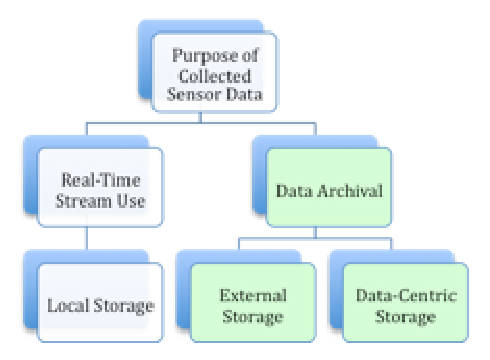
\includegraphics{../diagrams/taxonomy-data-purpose}
  \caption{The Purpose of Sensor Data Taxonomy}
  \label{fig:taxonomy-data-purpose}
\end{figure}

\begin{itemize}
  \item \textbf{Real-time Data Stream}: the collected data is accessed
  on-the-fly from the sensor device as a real-time data stream, and may have a
  short life cycle as it temporarily resides in memory;
  \item \textbf{Data Archival}: the collected data is used for historical
  purposes and is related to the historical data analysis \cite{sn-intro01,
  sn-intro02} or Information Fusion \ref{sn-info-fusion}. 
\end{itemize}

\section{The Location of the Sensor Data Taxonomy}

The location where the collected data is stored plays an important role
in the different aspects of the access to the collected data from sensor
devices, as shown in section \ref{sec:sn-storage-locations}. In this way,
Figure \ref{fig:taxonomy-data-location} depicts this taxonomy, which can be
described as follows:

\begin{figure}[h]
  \centering
  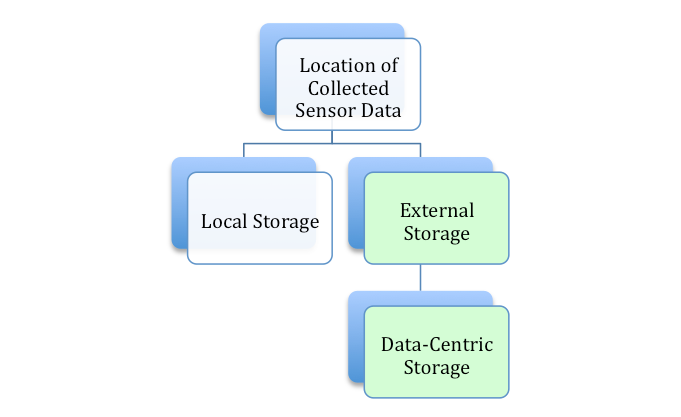
\includegraphics{../diagrams/taxonomy-data-location}
  \caption{The Location of Sensor Data Taxonomy}
  \label{fig:taxonomy-data-location}
\end{figure}

\begin{itemize}
  \item \textbf{Local Storage}: characterizes the placed of the collected data
  temporarily located in-memory, or in a secondary storage device on a node
  located in-network;
  \item \textbf{External Storage}: The collected data is usually located in an
  external storage device with a data management system such as a relational
  database;
  \item \textbf{Data-Centric Storage}: when the collected data occupies
  different external storages, being organized by categories based on the
  collected data keys and values. In other words, what characterizes this taxon
  is the presence of a data partitioning strategy to store the collected data.
\end{itemize}

\section{Data Model Taxonomy}

One of the fundamental challenges in the development of a persistence storage
in sensor networks is related to the data model chosen to represent the
collected data. Different data models were reported in the review of related
literature in section \ref{sec:data-models}. As a consequence, this taxonomy
relates to the data model used to design the collected data, as drawn in Figure
\ref{fig:taxonomy-data-model}, and described as follows.

\begin{figure}[h]
  \centering
  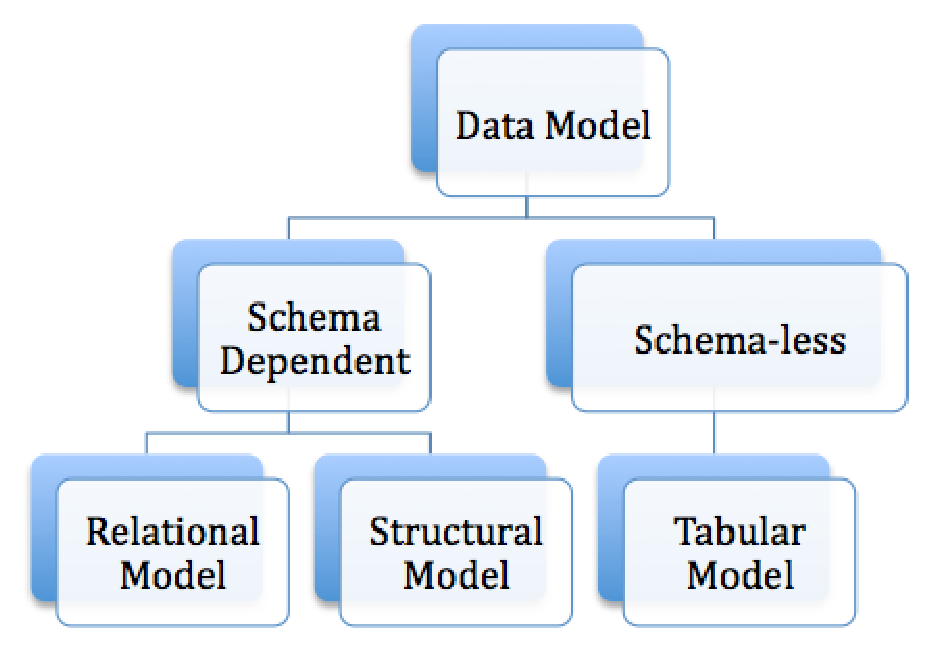
\includegraphics{../diagrams/taxonomy-data-model}
  \caption{Data Model Taxonomy}
  \label{fig:taxonomy-data-model}
\end{figure}

\begin{itemize}
  \item \textbf{Schema-Dependent Models}: this data model requires the
  definition of a master schema that describes the data through a rigorous of 
  data modeling process prior to the insertion of the data. Examples of such
  model is the traditional Relational Data Model\cite{relational-model}, as
 well as the Structured Data Models such as the XML \cite{xml};
  \item \textbf{Schema-less Models}: contrary to the former taxon, schema-less
  data models do not require the definition of a data schema or table
  definition. Instances of such data model reviewed in the literature review
  is the use of the Tabular Data model.
\end{itemize}

\section{Data Provenance Taxonomy}

No matter which data model used to represent the collected data, Data
Provenance provides a valuable guideline on how to describe the collected data
from sensors devices. As reported in section \ref{sec:sn-provenance}, the
description of the properties should take into account different properties of
the nature of the data as shown in Figure \ref{fig:taxonomy-data-provenance}.
Those taxa are summarized as follows:

\begin{figure}[h]
  \centering
  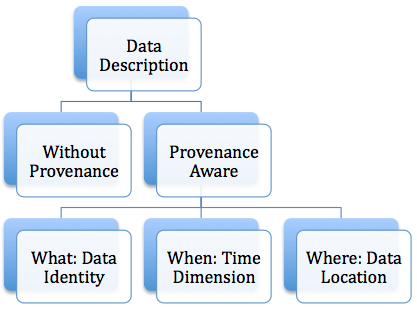
\includegraphics{../diagrams/taxonomy-data-provenance}
  \caption{Data Provenance Taxonomy}
  \label{fig:taxonomy-data-provenance}
\end{figure}

\begin{itemize}
  \item \textbf{What: Data Identity}: the data type that uniquely identifies
  the collected data from sensors. First and foremost, the properties of the
  sensor devices must be described according to the meaningful naming
  convention for the property. For instance, ``Water Temperature'' better
  describes the intent of the property as ``temp''. Second, the identification
  of the collected data related to the sensor type should be given, that is,
  which sensor device created the collected data, in case the data origin is
  relevant;
  \item \textbf{When: Time Dimension}: time is an important attribute of the
  data because it identifies the age of the collected data. Depending on the 
  use of the collected data, this is often taken into account. Two different
  types of time dimensions were described: \textbf{fact} and
  \textbf{transaction} times. The former is used to identify when the data
  was collected, whereas the latter when the data was transmitted to the
  data sink where the query processing acts;
  \item \textbf{Where: Data Location}: the point where the collected data was
  observed by the sensor device. Usually the latitude and longitude as the GPS
  coordinates are provided by devices which are capable of sensing the
  location. A descriptive metadata about the location could also be given such
  as room-name = ``deep see''.
\end{itemize}

\section{Query Processing Mechanism Taxonomy}

The query processing mechanism in sensor networks is directly related to how
and where the collected data is used and stored, as shown in section
\ref{sec:query-process}. As a consequence, the following taxa are related to the
different types of query processing mechanisms and summarized in Figure
\ref{fig:taxonomy-query-mechanism}:

\begin{figure}[h]
  \centering
  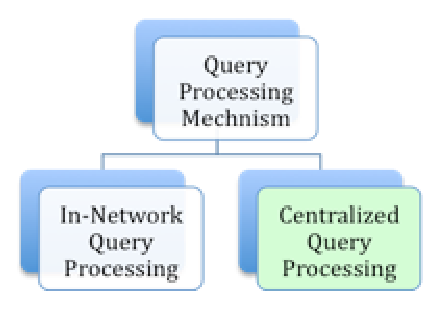
\includegraphics{../diagrams/taxonomy-query-mechanism}
  \caption{Query Processing Mechanism Taxonomy}
  \label{fig:taxonomy-query-mechanism}
\end{figure}

\begin{itemize}
  \item \textbf{In-Network Query Processing}: when the data node is the
  sensor device itself, and it uses the local storage mechanism, then the
  sensor node is able to reply to request related to the observations of the 
  environment defined by the sensor device. In this way, the query takes 
  place in the network itself, and usually returns values related to the current
  state of the environment;
  \item \textbf{Centralized Query Processing}: as developed by a single 
  relational database server, the data queried from a centralized data
  network sink in order to be reused. In general, this approach is used when
  the purpose of data is archival data.
\end{itemize}

\section{Database System Organization Taxonomy}

Different approaches of data systems were described in the literature review in
the last chapter in different sections. This taxonomy is directly related to
the use of external storage devices on a centralized network node so that it
often uses a single database server. Paradoxically, the use of a data-centric
storage determines the use of distributed database nodes around the network. 
In this way, Figure \ref{fig:taxonomy-database-architecture} describes the
taxonomy of the database system organization as follows:

\begin{figure}[h]
  \centering
  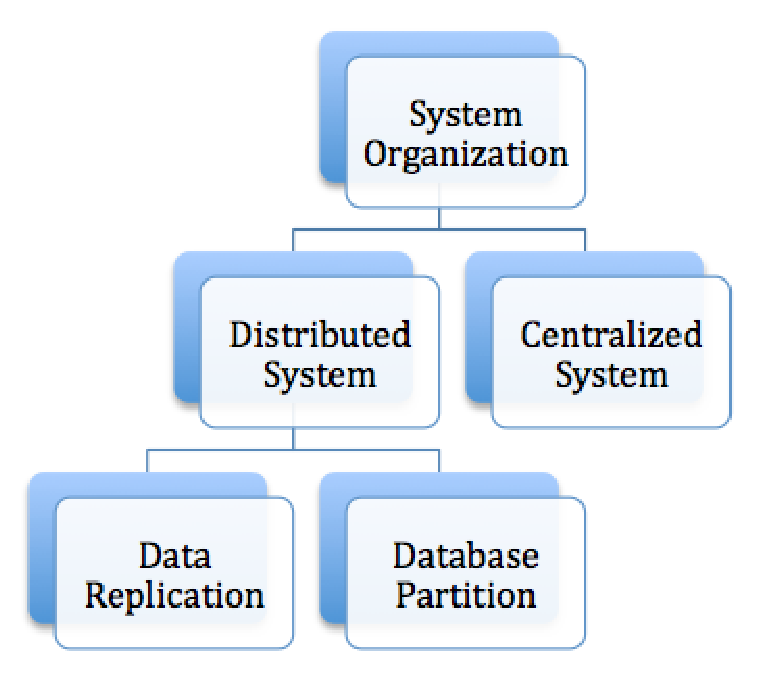
\includegraphics{../diagrams/taxonomy-database-architecture}
  \caption{Database Architecture Taxonomy}
  \label{fig:taxonomy-database-architecture}
\end{figure}

\begin{itemize}
  \item \textbf{Centralized System}: a database system that runs in one single
  centralized host, being the focal purpose of data traffic as read and writes 
  \cite{sn-intro01};
  \item \textbf{Distributed System}: a database system that can be composed by
  more than one node. Usually, the use of the pattern of Master-Slave
  mechanism or data ``Replication" is used. Another mechanism is the use of
  database paritioning, if the technology supports it.
\end{itemize}

\section{Relationships among the Taxonomies}

The different taxonomies defined in the previous sections of this chapter are
important to the understanding of a data persistence layer for sensor
networks. As they are closely related to each other, it is important to
briefly highlight these relationships in order to better analyze a problem
related to data persistence. 

The taxonomy related to the purpose of the sensor data can be directly related
to the taxonomy of the location of the sensor data. While the taxon of the 
real-time data stream relates to the local data storage, the taxon related to
data archival correlates the storage of the collected data into an external
storage. In addition to that, the converse is also true.

The taxonomy related to the data model can be related to any taxon from the
taxonomy of the location of the sensor data, as well as the taxons related to
Data Provenance. In the former, the data of a relational model is stored using
SQL messages.

In the light of these taxonomies, the classification of the data persistence
properties of a sensor networks can be studied and reviewed. As described in
the introduction of this dissertation, one the main motivations for this work
was to provide means of data persistence of NetBEAMS, a case study which does
not contain a data layer. Therefore, the following chapter seeks to describe
that case study in order to make a section of a given technology for evaluation.

% main.tex, to be used with thesis.tex
% This contains the main work of your thesis.

%\bibliography{thesis}  % uses the references stored in Chapter1Radar.bib

\chapter{Data Persistence for Sensor Networks: A Case Study for NetBEAMS}
\label{chap:netbeams-overview}

As discussed in Chapter 2, different properties of a sensor network and the
nature of the collected data must be taken into account in order to provide a
data persistence layer for a given sensor network. Similarly, in order to
better assist one's analysis of such functionality, Chapter 3 proposed a set of
data persistence taxonomies related to different properties of the collected
data life cycle. The goal of this chapter is to describe the fundamental properties 
of the case study used for this work, that is, NetBEAMS, in order to lay the 
groundwork as it relates to the selection of the database technology. NetBEAMS 
provides an automated infrastructure solution for SF-BEAMS, and this last component 
will be covered first. Then, this work proposes a categorization of NetBEAMS
according to the defined taxonomies.

\section{SF-BEAMS: a Marine Sensor Network for Water Quality Monitoring}

As described by \cite{netbeams2009}, NetBEAMS is a joint venture between the
department of Biology and Computer Science at San Francisco State University,
whose goal is to automate the operational execution of SF-BEAMS. The San Francisco
Bay Environmental Assessment and Monitoring Station, or SFBEAMS \cite{sfbeams2006}, 
is an environmental sensor network system whose primary focus is the study of complex 
marine and estuarine environments using the SF-BEAMS sensors. The sensors are deployed off a
pier located in the San Francisco Bay, in Tiburon, California; and is operated by 
the Romberg Tiburon Center for Environmental Studies (RTC) a part of San Francisco
State University. NetBEAMS is an experimental component that utilizes the SF-BEAMS 
infrastructure to operate. This section details SF-BEAMS in general, and
presents the requirements for data persistence after classifying NetBEAMS based
on the taxonomies defined in the previous chapter.

\subsection{The SF-BEAMS Infrastructure}
\label{sec:sfbeams}

The SF-BEAMS sensor network is responsible for providing data for water quality
monitoring, as well as weather and surface conditions. Figure
\ref{fig:sf-beams} shows a picture taken from the SF-BEAMS web-camera.

\begin{figure}[!t]
  \centering
    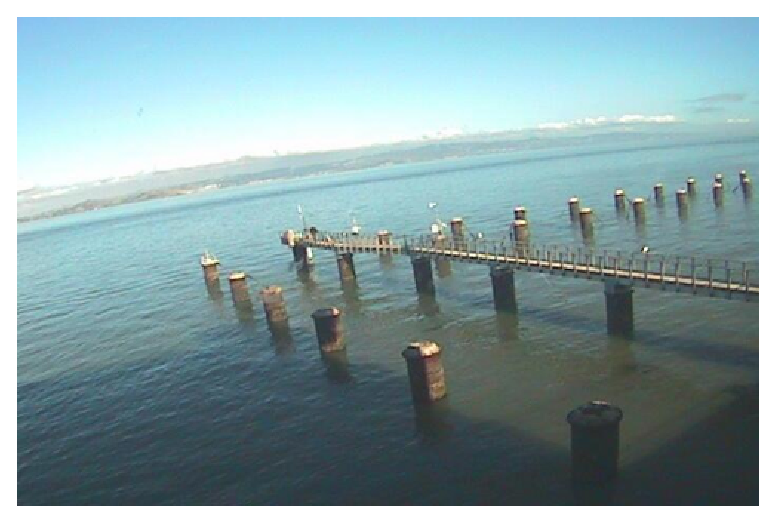
\includegraphics[scale=0.7]{../diagrams/cam_image-oct15}
  \caption{Picture of the SF-BEAMS Network, at the RTC pier. Tiburon, CA.}
  \label{fig:sf-beams}
\end{figure}

In general, the SF-BEAMS network infrastructure contains a varying number of
wired and wireless devices attached to pylons at the pier. Each of them
is responsible for observing different conditions of the area, having its own
mechanisms for internal storage for the collected data. In this way, data can
be directly transferred to the labs via Ethernet cables or collected manually
with a laptop computer. The current data collection process for SF-BEAMS is
described in Figure \ref{fig:SF-BEAMS-system-architecture} and documented at
\cite{sfbeams-current-system}. Upon collecting data from sensors, the RTC
staff uses automation scripts written in Matlab \cite{matlab} to process,
index and distribute the raw data in different formats. One of these formats
is the OPeNDAP \cite{opendap}, which is widely used at research institutions
to promote easier data exchange amongst them. The SF-BEAMS website provides
access to the collected data through the Internet at
http://sfbeams.sfsu.edu:8080/opendap. An example of an HTTP Request from
accessing the data for a specific device is shown in Listing
\ref{file:rtc-ysi-opendap} on page \pageref{file:rtc-ysi-opendap}.

\begin{figure}[!b]
  \centering
  \includegraphics[scale=0.5]{../diagrams/SF-BEAMS-system-architecture}
  \caption{The Current SF-BEAMS Data Collection Process}
  \label{fig:SF-BEAMS-system-architecture}
\end{figure}

As described in Section \ref{sec:sn-infrastructure}, sensor devices produce
the observed data based on properties of measurements defined by its
manufacturer. SF-BEAMS has used, among other devices, the ``6600 ESD V2" Sonde
\cite{YSI-Sonde}, manufactored by YSI Incorporated, as seen in Figure
\ref{fig:ysi-device}. Although it is a small device of under 55 cm in length,
8.9 cm in diameter, and weighting approximately 3.18 kg, it is a powerful water
quality-monitoring device, capable of producing around 52 bytes on a single
real-time data stream reading regarding 12 different parameters such as water
temperature, salinity, turbiny, among others. An example of the data stream is
as shown in Listing \ref{data:ysi-stream} on page \pageref{data:ysi-stream}.

\begin{figure}[!b]
  \centering
  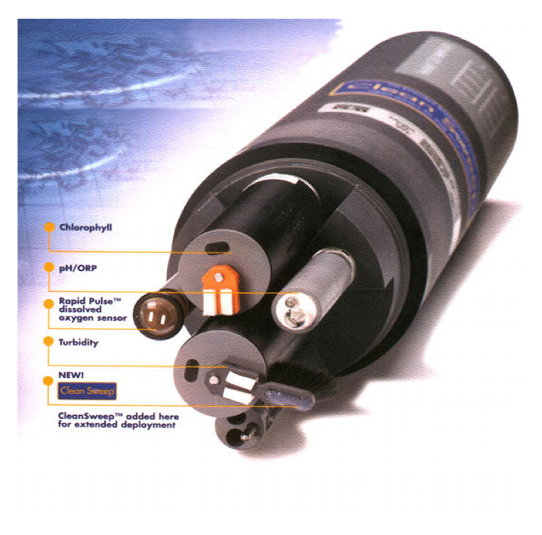
\includegraphics[scale=0.7]{../diagrams/ysi-device}
  \caption{Picture of the case study Sonde device: YSI 6600 ESD V2}
  \label{fig:ysi-device}
\end{figure}

\lstset{label=data:ysi-stream,caption=The Collected Data Stream from the
YSI Sonde 6600ESDV2}
\begin{lstlisting}
12.20    192    179 5588.40   0.09   0.084   0.059  7.98   -79.6   99.5  8.83  0.4     8.7
\end{lstlisting}

In order to have access to the observed data, the RTC network staff downloads
the data using one of the device's connections such as the RS-232 serial connector
\cite{rs232}. Then, they upload the data into their data servers where they are
processed and archived for historical analysis. According to one
staff member, the infrastructure of the SF-BEAMS is comprised of the 
following components (as of May 2009):

\begin{itemize}
  \item 5 YSI Sonde devices, among others, in operation at the RTC pier;
  \item The sampling frequency rate is configured in ranges of either 1, 6 or
  15 minutes, depending on the specification;
  \item The processed data, used for distribution over the Internet,
   contains information regarding the time of the data collection.
\end{itemize}

Considering the infrastructure, the data load in the server-side
of RTC's laboratories produced by the YSI Sonde sensors devices can be
estimated by analyzing the data distribution over a period of one year, as
shown in Table \ref{tab:year-data-distribution}.

\begin{table}[!b]
    \label{tab:year-data-distribution}
     \begin{center}
      \begin{tabular}{|c|c|c|c|c|c|c|}\hline 
        \textbf{\# of YSIs} & \textbf{Rate} & \textbf{Hourly} &
        \textbf{Daily} & \textbf{Weekly} & \textbf{Monthly} & \textbf{Yearly}\\\hline 
        1 & 1 min & 3.04 Kb & 73.12 Kb & 511.87 Kb & 1.99 Mb & 23.99 Mb\\\hline 
        5 & 6 min & 15.23 Kb & 365.62 Kb & 2.5 Mb & 9.99 Mb & 119.97 Mb\\\hline 
        1 & 15 min & 0.5 Kb & 12.18 Kb & 85.31 Kb & 341.25 Kb & 3.99 Mb\\\hline 
        5 & 1 min & 2.54 Kb & 60.93 Kb & 426.56 Kb & 1.67 Mb & 19.99 Mb\\\hline
        1 & 6 min & 0.2 Kb & 4.87 Kb & 34.12 Kb & 136.5 Kb & 1.6 Mb\\\hline 
        5 & 15 min & 1.0 Kb & 24.37 Kb & 170.62 Kb & 682.5 Kb & 7.99 Mb\\\hline
        \end{tabular}
        \caption{Estimated data volume produced by the RTC's YSI sondes}
      \end{center}
\end{table}

The maximum amount of data produced by the YSI Sonde device is hundreds of Megabytes
a year, as \textbf{483,840} samples are generated by one single device. 

\subsection{Taxonomic Classification of SF-BEAMS}

This section classifies the sensor network deployed by SF-BEAMS according to
the taxonomies proposed in the previous chapter. This classification is
necessary to better understand the requirements of a data persistence for
NetBEAMS, which indirectly uses the infrastructure of SF-BEAMS.

\begin{itemize}
  \item \textbf{The Purpose of Sensor Data}: the data from SF-BEAMS is exclusively
  used for the purpose of Data Archival, since they are stored in RTC's lab;
  \item \textbf{The Location of the Sensor Data}: it is clear that the purpose
  of the data is directly related to the sensors location and, thus, the
  strategy of \textbf{External Data Storage} is used to store its collected
  data at the network sink at the RTC site;
  \item \textbf{Data Model}: since the format used by the RTC staff to share
  data with researchers is in the OPeNDAP format, the data
  model used is the tabular data model, since it uses the comma-delimited
  files. In this way, the \textbf{Schema-less} model is used;
  \item \textbf{Data Description}: once the collected data reaches the RTC
  lab, a quality assurance process is executed, and the data is transformed
  into the format used by OPeNDAP. The process to describe the collected data
  includes the time of the data collection, therefore, one of the \textbf{Time
  Dimensions} such as the valid time is used. Since the files are stored with
  specific file name structure, using timestamps to describe the data, the use
  of transaction time may be also considered. Finally, the contents of the
  files contain the \textbf{Data Identity} as shown in the samples of the
  collected data in Listing \ref{file:rtc-ysi-opendap} on page
  \pageref{file:rtc-ysi-opendap};
  \item \textbf{Query Processing Mechanism}: similar to the data stored in a
  centralized way, the query processing is also \textbf{Centralized}, as the
  data is stored on file system;
  \item \textbf{Data Volume}: the volume of data produced is characterized by small.
 It is related to the volume of data produced by the sensor devices,
  which is numerical data streams, and the total number of sensor devices;
  \item \textbf{System Organization}: SF-BEAMS runs on a Single System, as
  the collected data is stored directly in the file-system after previous 
  processing. However, the collected data is provided to the Internet using
  the OPeNDAP Hyrax system as a middleware.
\end{itemize}

\section{NetBEAMS: a component-based approach for SF-BEAMS}
\label{sec:problem-requirements}

Although the execution of RTC's sensor network can be operated as it
was mentioned in the previous sections, \cite{netbeams2009} described some of the
operational challenges faced by the RTC staff during regular activities of the
data collection process. It was clear to the research group that SF-BEAMS
could have not only its data gathering process automated, but also its data
management and distribution. By the use of COTS\footnote{Common-Off-The-Shelf
designates a product that is produced and sold in bulk} embedded devices and
open-source \cite{open-source} software, the research group developed NetBEAMS,
component-based approach which suggested the improvement of operational
activities from SF-BEAMS using systems automation. In brief, one of the
ongoing problems of NetBEAMS was regarding Data Persistence, the primary
motivation of this report.

The Networked Bay Environmental Assessment and Monitoring System, or Net-BEAMS,
offers the Data Sensor Platform (DSP) \cite{netbeams2009} as the system
architecture that can address the operation of SF-BEAMS. The in-depth
documentation describing the DSP Platform, including its architecture and data
gathering process is provided at the online documentation 
\cite{netbeams-dsp-architecture}.

The scope of this work is defined as to provide a persistence layer for
NetBEAMS, making a selection of a persistence layer based on the taxonomical
classification of SF-BEAMS. Furthermore, the technology to be selected for the
persistence layer must take into account the requirements of NetBEAMS primary
users such as Computer Science researchers, as well as end users such as
Biologists from the RTC laboratories. The requirements for the data
persistence specifically for NetBEAMS are described in the following section.

\section{Requirements for NetBEAMS Data Use}

The main reason for the operation of SF-BEAMS using NetBEAMS's automated
approach is that it can potentially reduce operational costs and improve the
data collection process. In view of this, the scope of a persistence layer
can be summarized as a group of functional and non-functional requirements in
order to select a database system for the sensor network supported by NetBEAMS.

\subsection{Functional Requirements}

\begin{itemize}
  \item Reuse the NetBEAMS infrastructure and develop a component responsible
  for data persistence in a database system;
  \item The Persistence System must obey to the characteristics of the
  categorization of SF-BEAMS used by the taxonomies.
\end{itemize}

\subsection{Non-Functional Requirements}

\begin{itemize}
  \item The data model used to describe the data must not impose restrictions
  to the users of the system (i.e. Biologists and students without expertise in
  Database Systems);
  \item Data Representation must be similar to those used by RTC, with a
  more human-readable format;
  \item The system must be scalable with a low degree of maintenance, in a
  way that the interruptions to the data gathering process are infrequent;
  \item Data must be searchable in near-real-time with good performance;
  \item The system must also support export capabilities, which may
  be used to match RCT's requirements of the OPeNDAP format;
  \item The database must be free of charge, following the
  implementation specifications of NetBEAMS for Open-source software.
\end{itemize}

In conclusion, after detailing the SF-BEAMS sensor network, and describing the 
infrastructure of NetBEAMS, its the motivation and goals for this project were 
presented. The next chapter is the actual analysis of existing database systems 
mentioned in Chapter 2, which aligns with the requirements and characteristics of 
NetBEAMS. Meanwhile, more details regarding the architecture of NetBEAMS, as well as
the development guidelines can be found in the appendix of chapter 10.

% main.tex, to be used with thesis.tex
% This contains the main work of your thesis.

%\bibliography{thesis}  % uses the references stored in Chapter1Radar.bib

\chapter{Data Persistence Technology for Sensor Networks: An Empirical-based
Choice for NetBEAMS}

This chapter analyzes each of the taxonomies defined in chapter
\ref{chap:taxonomies} against the requirements defined by our case study,
NetBEAMS, in chapter \ref{sec:problem-requirements}. Moreover, it evaluates
different database technologies against on those taxonomies, and tries to select
one of them which can be a candidate for an experimental analysis.

First, the contender technologies are as follows:

\begin{itemize}
  \item MySQL
  \item Microsoft SQL 
  \item Berkeley TinyDB
  \item MongoDB
  \item CouchDB
  \item IBM DB2
\end{itemize}


\section{Analysis of the Purpose of Sensor Data Taxonomy}

Considering the infrastructure of NetBEAMS, as described in the previous
chapter, and the characteristics of the sensor network defined at the SF-BEAMS
\cite{sfbeams2006} site, the data characteristics are as follows:

\begin{itemize}
  \item Data is generated by sensor devices, such as the YSI sonde
  \cite{YSI-Sonde}, and manually collected by using a laptop to the network
  sink at the RTC laboratories;
  \item Upon data reception, the RTC staff index and archive the data for
  for distribution using the OPEnDAP format;
  \item Another approach for data collection of data generated by the SF-BEAMS
  is the use of NetBEAMS \cite{netbeams2009}, as described in section
  \ref{netbeams-architecture}.
\end{itemize}

Given the facts collected from the observations of the execution of NetBEAMS
through the SF-BEAMS sensor network, we can say that the purpose of collected
data is \textbf{Data Archival}.

\subsection{Technology Analysis}

Any of the contenders are options to cover for Data Archival.

\begin{itemize}
  \item \textbf{MySQL}: Supports
  \item \textbf{Microsoft SQL}: Supports
  \item \textbf{Berkeley TinyDB}: Supports
  \item \textbf{MongoDB}: Supports
  \item \textbf{CouchDB}: Supports
  \item \textbf{IBM DB2}: Supports
\end{itemize}

\section{Analysis of the Location of Sensor Data Taxonomy}

Some observations regarding the location of the collected sensor data for
NetBEAMS were described in the previous section and summarized as follows:

\begin{itemize}
  \item NetBEAMS's architecture is based on a single-hop star infrastructure 
   with a direct network sink being the RTC server \ref{sec:sn-infrastructure}.
\end{itemize}

Based in the observations described, the type used for storing
data can be either the \textbf{External Storage} or the
\textbf{Data-Centric Storage}. The former is the current approach used by the
SF-BEAMS sensor network, while the latter adopted as an improvement of the
persistence infrastructure for NetBEAMS.

\subsection{Advantages of the External Storage Approach}

The External Storage approach is the most common way to implement persistence
for any type of systems, including sensor networks, due to its the simplistic
data management. Furthermore, this type of setup is easier to use of
distributed systems approaches such as Replication to help preventing scaling
the system.

\subsection{Disadvantages of the External Storage Approach}

The most common problem related to a single External Data Storage is that
resources may run into data management problems such as full disk space or disk
failures.

\subsection{Advantages of the Data-Centric Approach}

The advantage of the Data-Centric approach lies on the way that data is
distributed into different locations. By using techniques of distributed
database systems, the approach improves overall performance of the use of
massive data sets since the operations of the data are directed to specific
locations. Besides, this approach helps the network managers scale the data
storage just by adding new data nodes as required.

\subsection{Disadvantages of the Data-Centric Approach}

The data partitioning is a very restricted technology, mostly available to
advanced users of distributed database systems. The main users of wireless
sensor networks do not have such expertise.

\subsection{Technology Analysis}

\begin{itemize}
  \item \textbf{MySQL}: Supports
  \item \textbf{Microsoft SQL}: Supports
  \item \textbf{Berkeley TinyDB}: Supports
  \item \textbf{MongoDB}: Supports
  \item \textbf{CouchDB}: Supports
  \item \textbf{IBM DB2}: Supports
\end{itemize}

\section{Analysis of the Query Processing Mechanism Taxonomy}

As a direct result from the previous section, the use of \textbf{Centralized Query
Processing} is indicated for NetBEAMS, given the fact that NetBEAMS contains
a single network sink, and therefore, a centralized location of the data.

\subsection{Advantages of the Centralized Query Processing}

Centralized data management and query processing is simpler than in in-network.
The centralized query processing can be 

\subsection{Disadvantages of the Centralized Query Processing}

The creation of the so-called Funneling Affect, since the point-of-traffic is
concentrated in the centralized system. Any data exchange will be using the
same channel of data exchange.

\subsection{Technology Analysis}

\begin{itemize}
  \item \textbf{MySQL}: Supports
  \item \textbf{Microsoft SQL}: Supports
  \item \textbf{Berkeley TinyDB}: Supports
  \item \textbf{MongoDB}: Supports
  \item \textbf{CouchDB}: Supports
  \item \textbf{IBM DB2}: Supports
\end{itemize}

\section{Analysis of the Data Model Taxonomy}

One of the most common practices in the area of database system is to use the
relational model to persist data, although the application of the system may
not fit to solve the problem. In fact, the main users of sensor networks may
not hold any expertise in database systems or data modeling, given they come
from different science areas. Taking NetBEAMS as an example, we see a Sensor
Network managed by Marine Biologists without expertise in Data Management,
Modeling systems, and for this reason, one of the requirements of the system is
the use of schema-less approaches. The \textbf{Key-Value-Pair Data Model} or the
\textbf{Document-Oriented Data Model} seems to be the simplest choices of the
models.

\subsection{Analysis of the Schema-Dependent Models}

Considering the inception of a relational data model \cite{relational-model} and
the use of the YSI Sonde data as the main entity in the system, let figure 
\ref{fig:Relational-Model-Original} represent a prototype of the relational
model, after passing through the process of normalization
\cite{db-normalization}.

\begin{figure}
  \centering
  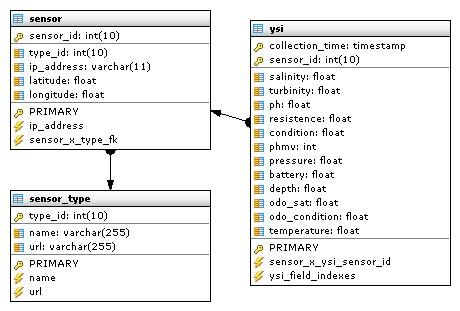
\includegraphics[scale=0.65]{../diagrams/Relational-Model-Original}
  \caption{Relational Data Model for NetBEAMS - A first prototype}
  \label{fig:Relational-Model-Original}
\end{figure}

Supposing a new type is added into the system, let the refactored
version of the relational model be depicted in figure
\ref{fig:Relational-Model-Addition-Modified}.

\begin{figure}
  \centering
  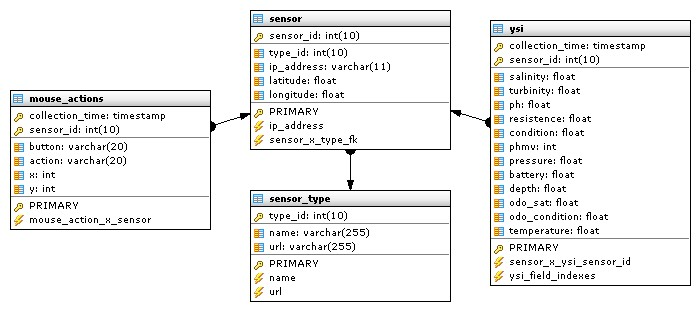
\includegraphics[scale=0.65]{../diagrams/Relational-Model-Addition-Modified}
  \caption{Relational Data Model for NetBEAMS - Modified version with new
  entity}
  \label{fig:Relational-Model-Addition-Modified}
\end{figure}

\begin{itemize}
  \item Constant data schema changes require constant database normalization
  process, changes to structure, database management, etc;
  \item Some research have shown that the Relational Model does not fit the
  nature of collected data from wired or wireless sensor networks. They usually
  does not support time-series data nor provenance.
  \item Even project aiming at updating the relational sensor database systems
  and SQL clauses have been proposed. 
\end{itemize}

Other projects have been using the XML data models. It falls into the same
category as the Relational Model, since the XML documents, when in the context
of a database, must be complaint to an XML Schema. As shown in section 3, this
model uses XPath technology for querying documents, although some hibrid
technologies may still use SQL for that matter. In this way, an instance of
such schema dependent types can be seen in figure
\ref{fig:persistence-example-relational}.

\begin{figure}[!h]
  \centering
  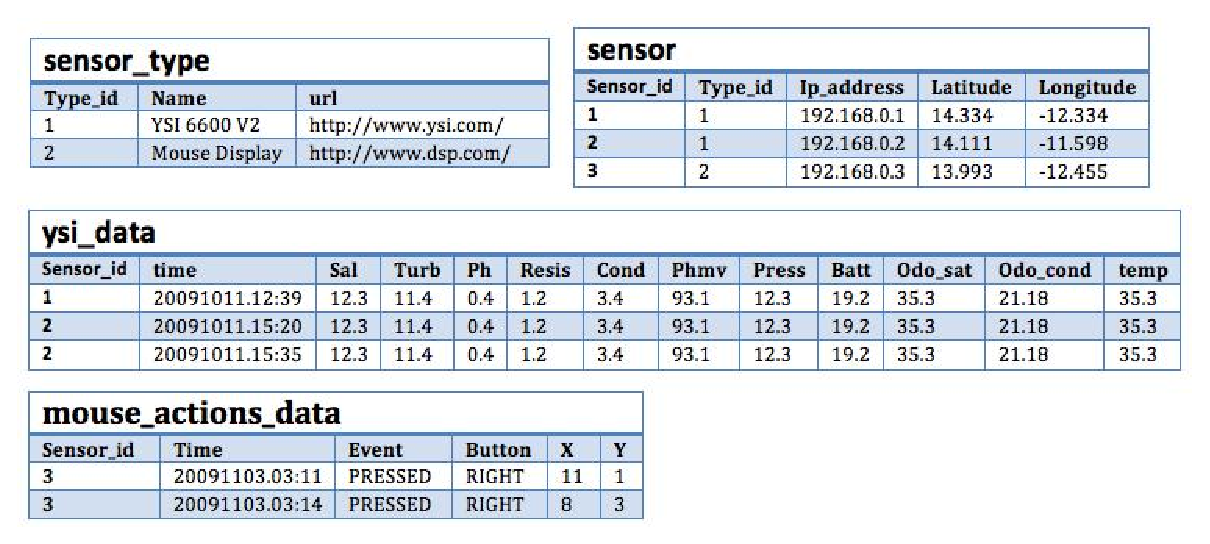
\includegraphics[scale=0.65]{../diagrams/persistence-example-relational}
  \caption{Instance of a Relational Model Database Prototype}
  \label{fig:persistence-example-relational}
\end{figure}

Although this data model have been used in different types of applications,
developers have tried to use the Relational Model to model an application that
could prevent any database change through the use of a technique that relates a
key to a value, called Key-Value data model. With the advent of Internet
applications, the need of such a model that does not need constant refactoring
led developers to propose such approach using the relational model as
documented in technical articles such as \cite{db-kvp-in-relational01} and
\cite{db-kvp-in-relational02}. Based in these articles, consider the relational
model depicted in figure \ref{fig:KVP-on-Relational-Model} as model for the
persistence data for our case study using the key-value strategy. The problem
with it is that key repetition occurs, since the nature of time-series data
requires the use of a timestamp key for each property of the sensor. Therefore,
this strategy is not well-suited to provide persistence data from collected
sensor networks.

\begin{figure}[!h]
  \centering
  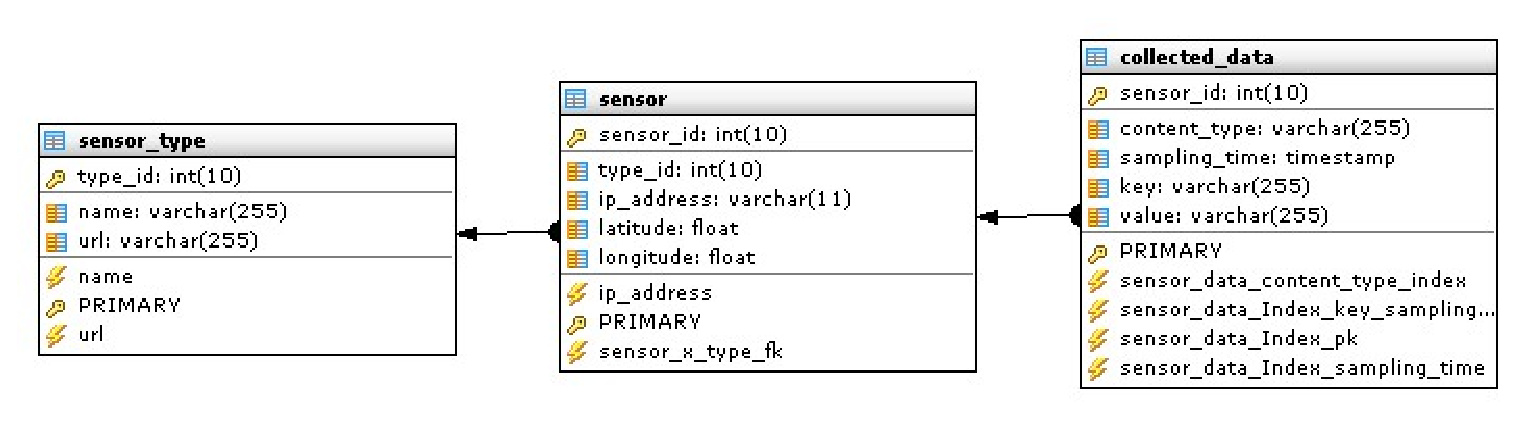
\includegraphics[scale=0.5]{../diagrams/KVP-on-Relational-Model}
  \caption{KVP Data Model implementation using Relational Model}
  \label{fig:KVP-on-Relational-Model}
\end{figure}

\begin{figure}[!h]
  \centering
  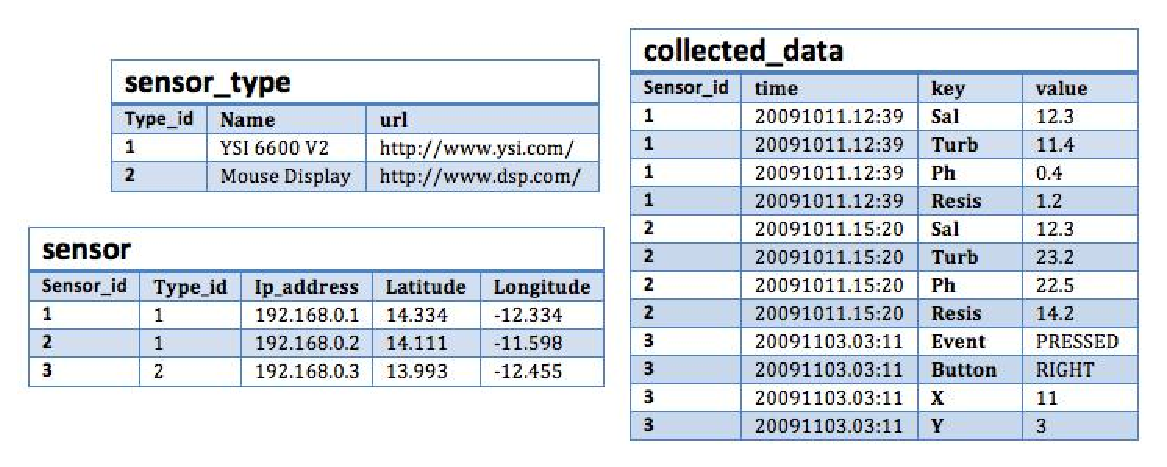
\includegraphics[scale=0.5]{../diagrams/persistence-example-relational-kvp}
  \caption{KVP over Relational Model Database Prototype}
  \label{fig:persistence-example-relational-kvp}
\end{figure}

\subsection{Analysis of the Schema-less Models}

The advance of Cloud Computing, and dynamic web applications have motivated the
database community to implement different mechanisms for persisting data
without the heavy-process of data modeling. Given the fact that sensor networks
may be updated at any time by the addition of new sensor types, the use of
moding approaches such as Key-Value Database have been proposed \cite{db-kvp}.

\begin{itemize}
  \item entities from the same domains are placed into a bucket;
  \item entities have a set of attributes and relating values
  \item entities with different set of attributes may be contained in the same
  bucket, since there is no schema to govern the bucket items restriction.
\end{itemize}

For instance, all data needed for the YSI sonde data, as well as all necessary
provenance data that describes the data, are represented by means of key-value
pairs \ref{fig:persistence-example-kvp}.

\begin{figure}[!h]
  \centering
  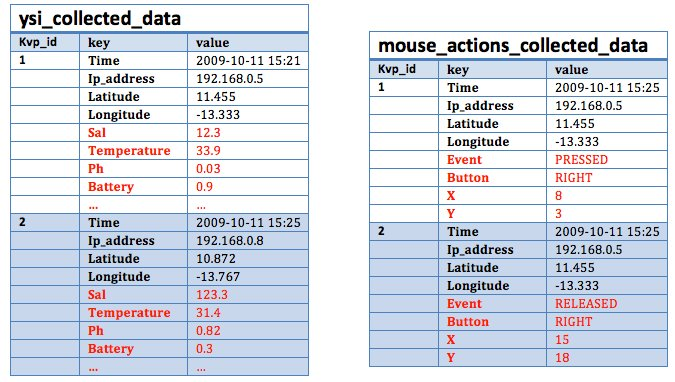
\includegraphics[scale=0.5]{../diagrams/persistence-example-kvp}
  \caption{KVP Database instance Prototype}
  \label{fig:persistence-example-kvp}
\end{figure}

\subsection{Technology Analysis}

The data models were compared by \cite{db-is-rdbs-dommed} and can be summarized
as follows:

\begin{table}
    \label{tab:ysi-data-distribution}
    \caption{Schema-Dependent X Schema-less Databases Compared: Properties}
    \begin{center}
    \begin{tabular}{|p{210pt}|p{210pt}|}\hline
    Schema-Dependent Databases & Schema-less Databases\\\hline
    \begin{enumerate}
      \item Real-world model by entities, classified in tables;
      \item Tables composed by columns and rows. Rows are comprised by column
      values, which have the same schema;
      \item Data Model defined in advance with a schema, which contains
      relationships and constraints to enforce data integrity;
      \item Data represents ``natural'' entities, not application specific;
      \item Data Normalization is the data structuring process to remove data
      duplication, as well as establishing data associations through table
      relationships.
    \end{enumerate} 
    & 
    \begin{enumerate}
      \item Real-world model by entities, classified in Domains;
      \item Domains are similar to tables, but like buckets that contains items
      without a pre-defined schema, what enable them to have different schemas;
      \item Items are identified by keys, as well as have a dynamic set of
      attributes attached to it, however with no schema defined;
      \item Items may represent not only the natural representation of data, but
      also include application-specific data;
      \item Since data may be repeated, no data normalization is done, so that
      integrity is done in the application layer.
    \end{enumerate}
    \\\hline
    \end{tabular}
    \end{center}
\end{table}

\begin{table}
    \label{tab:ysi-data-distribution}
    \caption{Schema-Dependent X Schema-less Databases: Data Access}
    \begin{center}
    \begin{tabular}{|p{210pt}|p{210pt}|}\hline
    Schema-Dependent Databases & Schema-less Databases\\\hline
    \begin{enumerate}
      \item The basic operations CRUD \footnote{Create-Retrieve-Update-Update
      database operations} data are performed using a structured language such
      as the SQL or XPath;
      \item Query languages can access data from different tables through
      joins, contains functions for aggregation and complex filter.
    \end{enumerate} 
    & 
    \begin{enumerate}
      \item The CRUD operations are performed via API \footnote{Application
      Programming Interface} through programming languages;
      \item Some technologies provide basic SQL-like syntax for filter criteria
      with some predicates like =, !=, <, > that ca be applied;
      \item The data and application integrity logic is placed in the
      application layer.
    \end{enumerate}
    \\\hline
    \end{tabular}
    \end{center}
\end{table}

\begin{table}
    \label{tab:ysi-data-distribution}
    \caption{Schema-Dependent X Schema-less Databases: Application Interface}
    \begin{center}
    \begin{tabular}{|p{210pt}|p{210pt}|}\hline
    Schema-Dependent Databases & Schema-less Databases\\\hline
    \begin{enumerate}
      \item Have their own specific API or through ODBC\footnote{Open Database
      Connectivity};
      \item Data is stored in a format that represents its natural structure,
      and for this reason, in a single or distributed fashion.
    \end{enumerate} 
    & 
    \begin{enumerate}
      \item Systems tend to provide SOAP/REST \cite{http-rest};
      \item \cite{db-is-rdbs-dommed} claims that data is stored in a more
      effective way, requiring only code plumbing for the relational code;
    \end{enumerate}
    \\\hline
    \end{tabular}
    \end{center}
\end{table}

\begin{itemize}
  \item MySQL: NO SUPPORT
  \item Microsoft SQL: NO SUPPORT
  \item Berkeley TinyDB: NO SUPPORT
  \item \textbf{MongoDB}: Supports Both
  \item \textbf{CouchDB}: Supports Both
  \item IBM DB2: NO SUPPORT
\end{itemize}

\section{Analysis of the Database System Organization Taxonomy}

Sensor Network data can be saved in either Centralized or Distributed Systems.
While Centralized Database Systems are easier to manage, it may face challenges
regarding its data. For this reason, the use of partitioning or sharding would
be an addition to persist sensor data.

\subsection{Advantages of Database Partitioning and Sharding}

\begin{itemize}
  \item Data-Centric queries and data use;
  \item Solves bottleneck problems related to reads/writes;
  \item Decrease the funneling effect by directing queries to given data
  partition;
\end{itemize}

\subsection{Disadvantages of Database Partitioning and Sharding}

\begin{itemize}
  \item Very advanced topics in Database System;
  \item May be easy of use, depending on the application.
\end{itemize}

\subsection{Technology Analysis}

\begin{itemize}
  \item \textbf{MySQL}: Supports
  \item \textbf{Microsoft SQL}: Supports
  \item \textbf{Berkeley TinyDB}: NO Supports
  \item \textbf{MongoDB}: Supports
  \item \textbf{CouchDB}: Supports
  \item \textbf{IBM DB2}: Supports
\end{itemize}

\section{Other Non-Functional Analysis}

\begin{itemize}
  \item Given the fact of the nature of the project, the technology to be used
  must be \textbf{open-source} \cite{open-source}, that is, no costs involved
  in the adoption of such technology;
  \item A solution for persisting collected sensor data must be not only limited
  to a technology that provides data access, such as SQL, but also by other
  \textbf{data access mechanisms} such as through \textbf{native APIs}. The
  reason is that part of the sensor network data does not have skills in
  database models, but may have skills with programming languages;
  \item Supports hot backup without service interruption.
\end{itemize}

\subsection{Technology Analysis}

Most of the technologies listed provides access to the data sets through the
use of drivers in different programming and scripting languages such as Java,
Python, Perl, etc.

\begin{itemize}
  \item \textbf{MySQL}: Supports
  \item \textbf{Microsoft SQL}: Supports
  \item \textbf{Berkeley TinyDB}: Supports
  \item \textbf{MongoDB}: Supports
  \item \textbf{CouchDB}: Supports
  \item \textbf{IBM DB2}: Supports
\end{itemize}

\section{Global Analysis Results and Technology Selection}

\begin{table}
    \label{tab:ysi-data-distribution}
    \caption{Amount of data produced by the RTC's YSI sondes}
        \begin{center}
        \begin{tabular}{|c|c|c|c|c|c|c|}\hline 
        \textbf{Database} & \textbf{MySQL} & \textbf{MicrosoftSQL} & \textbf{TinyDB} &
        \textbf{MongoDB} & \textbf{CouchDB} & \textbf{IBM DB2}\\\hline 
        Centralized Query & + & + & + & + & + & + \\\hline 
        Distributed System & ++ & ++ & - & ++ & ++ & +\\\hline 
        Schema-less & - & - & - & + & + & +\\\hline 
        Provenance Support & + & + & + & + & + & +\\\hline 
        NO-SQL Query & - & - & - & + & + & +\\\hline 
        Data Partition & + & + & - & + & + & +\\\hline 
        Hot Backup & + & + & - & - & - & +\\\hline 
        Export Capability & + & + & - & + & + & -\\\hline 
        Programming Lang. & + & + & + & + & + & +\\\hline
        Script Lang. & + & + & - & + & + & +\\\hline
        Open-Source & + & - & + & + & + & -\\\hline
        \end{tabular}
        \end{center}
\end{table}

% main.tex, to be used with thesis.tex
% This contains the main work of your thesis.

%\bibliography{thesis}  % uses the references stored in Chapter1Radar.bib

\chapter{DSP Data Persistence: Component Design and Architecture}

In order to provide data to users, the RTC scientists use OPeNDAP \cite{opendap}
server to distribute collected data over the Internet. However, this work
proposes the use a KVP database system as described in the previous chapter,
giving options to advanced techniques to scale on data structure and
organization.

This section shows the proposed DSP Data Persistence component for the DSP
Platform as reviewed in chapter 4, as it is responsible for gathering
the DSP Messages sent from any remote DSP instance. First, section 3.1 briefly
describes main events, processes, input and outputs generated by analyzing a
scenario of remote communications between sensors and the DSP Client and
Server nodes. Then, section 3.2 shows the requirements specification based on
the analysis of section 3.1 and the documentation of the DSP Platform of
section 2.4.

\section{Business Process Analysis}

As described in section 2.4, the Data Sensor Platform was designed to support
an environmental sensor network based in San Francisco Bay, composed by
different types of sensors. The process of extracting the measurements from the
sensors to be reused using the DSP Platform can be summarized following the UML
Business Process diagram depicted in figure
\ref{fig:fig:dsp-persistence-business-process}. It is important to note that
this diagrams details remote communication between sensor devices and a
centralized server, as part of the main scenario to solve the problem of data
persistence.

\begin{figure}[!b]
  \centering
  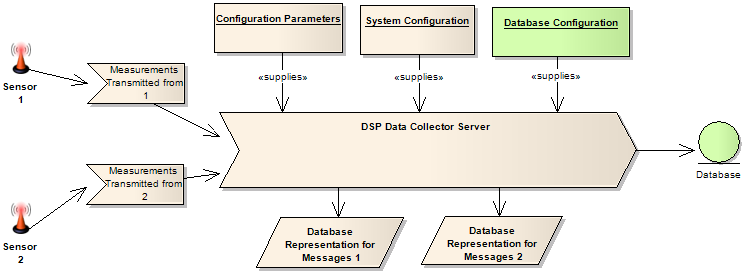
\includegraphics[scale=0.5]{../diagrams/DSP-DataPersistence-Business-Diagram}
  \caption{UML Business Process Model diagram - Adding Persistence for NetBEAMS}
  \label{fig:dsp-persistence-business-process}
\end{figure}

At the event of data collection, the DSP Client receives measurements collected
from each of the sensor devices. Each of the co-located DSP Client processes
the collected measurements and transforms them into the so-called DSP Message
(section 2.4), which embodies the actual data values. After proper data
processing, transformation and categorization, the DSP Message is added into an
in-memory data storage identified (section 2.4). Then, as an asynchronous data
transmission event occurs with an specified rate, transferring all the queued
messages to be processed by a DSP Server host. As it is detailed in image
3.1.1, the server is centralized and is able to concurrently process messages.

This work proposes the addition of a database system that is responsible for
storing the gathered measurement data from sensor hosts on a given network. As
it is shown in image 3.1.1,  the processed measurement data from sensors 1
through N must be collected in the same fashion and categorized as necessary.
In this way, end users such as Biologists and/or Programmers can access the
collected measurements directly from the Database. Furthermore, the same
measurement data is supposed to be exported to different formats as the users
find necessary.

As a matter of fact, the measurements data collected from the sensor devices
are simple  properties with and associated values as described on section 2.1.
According to the descriptions of the DSP Platform and the DSP Messages
structure on section 2.4, the data is represented in programming language
formats such as Java or in a serialized version in XML. Similarly, the
collected data contains measurements that uniquely identifies them, together
with other properties such as time stamps of data creation and collected, as
well as the the IP address of the DSP Client that produced the data. Therefore,
these are important properties for the proposed solution of this work.

\section{Requirements Specification}

By analyzing the main scenario of data process on section 3.1, this section
lists the main use cases that the system and the primary users require. One of
the primary requirements of the system is to enable the use a persistence
system that does not promote the use of specialized professionals to deal with
data modeling, as it is required in most projects using the Structured Query
Language (SQL) [db01], used to extract data from a Relational Database [db01].

\subsection{Functional Requirements}
As part of the user stories related to data access, figure
\ref{fig:DSP-Data-Persistence-UseCases-Diagram-Users} describes the use cases
that the end users can perform with the system.

\begin{figure}[!b]
  \centering
  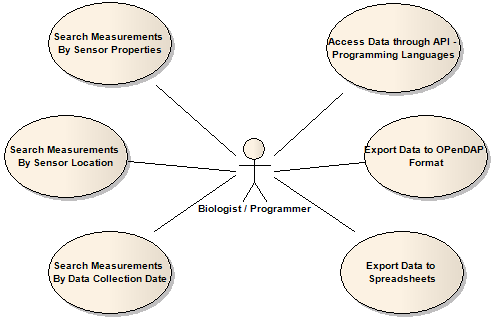
\includegraphics[scale=0.5]{../diagrams/DSP-Data-Persistence-UseCases-Diagram-Users}
  \caption{UML Use Case diagram for Persistence Functions}
  \label{fig:DSP-Data-Persistence-UseCases-Diagram-Users}
\end{figure}

The functional requirements listed in this section are in the format of UML
User Cases [se05]. Figure
\ref{fig:DSP-Data-Persistence-UseCases-Diagram-System} summarizes the use
cases that the system, as the main actor of the system, must perform:

\begin{figure}[!b]
  \centering
  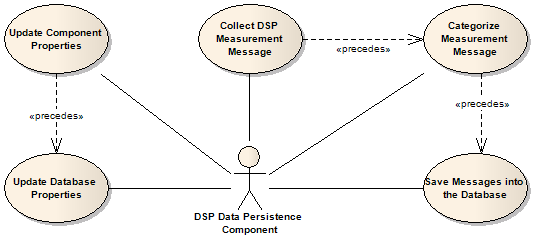
\includegraphics[scale=0.5]{../diagrams/DSP-Data-Persistence-UseCases-Diagram-System}
  \caption{UML Use Case diagram for System Persistence Functions}
  \label{fig:DSP-Data-Persistence-UseCases-Diagram-System}
\end{figure}

\subsection{Non-Functional Requirements}

\begin{itemize}
  \item The DSP Data Persistence component must maintain the received DSP
  Measurement Messages in-memory for a specific rate in order to decrease the
  write load on the database;
  \item The Persistence storage system must be able to cope with dozens of DSP
  Messages;
  \item The Persistence storage system must be able to save measurements quickly;
  \item The Persistence storage system must be able to scale without too much
  architectural changes;
  \item The Persistence storage system must not impose the knowledge of
  complicated database system languages such as SQL [db01] or XML XPath [db05],
  but use access through API calls, since it is closer to researchers. 
\end{itemize}
    
\section{Data Model Design}

After analyzing section 2.1 along with the functional and non-functional
requirements described on section 3.2.2, this work considered the
Key-Value-Pair Data model as described on Section 2.5. Taking into account the
mongoDB architecture and the properties of a DSP Message (see section
"Acquiring the properties of a DSP Message Content" at DSPDataPersistence),
here are the conventions followed on revision r585. The following is the list
of properties that composes the Key of a document:

\begin{itemize}
  \item \textbf{sensor\underline{ }ip\underline{ }address}: it's extracted from
  the DSP Message Produce and identifies which sensor generated the sampling;
  \item \textbf{message\underline{ }id}: it's extracted from each of the messages contained
  in the DSP Message Container;
  \item \textbf{transaction\underline{ }time}: it's extracted from the DSP message container
  creation time and it is used to identify when the transaction occurred (see Section 2.2);
  \item \textbf{fact\underline{ }time}: it's extracted from the SondeDataContainer's date
  and time, and identifies the time in which the collected data occurred (see Section 2.2);
  \item \textbf{latitude}: the latitude variable of the position;
  \item \textbf{longitude}: the longitude variable of the position.
\end{itemize}

The definition of the Value of a document is as follows:

\begin{itemize}
  \item data: this key defines the values of the document, and will have every
  different property of the sensor (see Section 2.4):
   \begin{itemize}
     \item battery
     \item temperature
     \item salinity
     \item \ldots
   \end{itemize}
\end{itemize}

Some remarks about the creation of the items contained with the collections. In
case a message container contains multiple readings in a message container,
each item will be counted as individual snapshots of the data. Also, it is
important to note that the description of the data follows no pattern other
than the description of the properties of the sensor device. However, some
studies have shown that when disk space maximization is required, the name of
database columns are important.

\section{High-Level System Architecture}

Considering the business analysis described in section 3.1, the addition of a
data persistence layer to the DSP Platform can be achieved by adding Data
Consumer (DC) as described in section 2.4. Based on the Requirements
specification described in section 3.2, this component must be responsible for
providing the processing of the DSP Measure Messages into Database-ready
representation, as well as providing the necessary tools for the transmission
of the data to a database system. Figure
\ref{fig:NetBEAMS-Persistence-Server-Node-Components} provides an
architectural view of the DSP Server node with the loosely-coupled components,
highlighting the inclusion of the DSP Data Persistence.

\begin{figure}[!b]
  \centering
  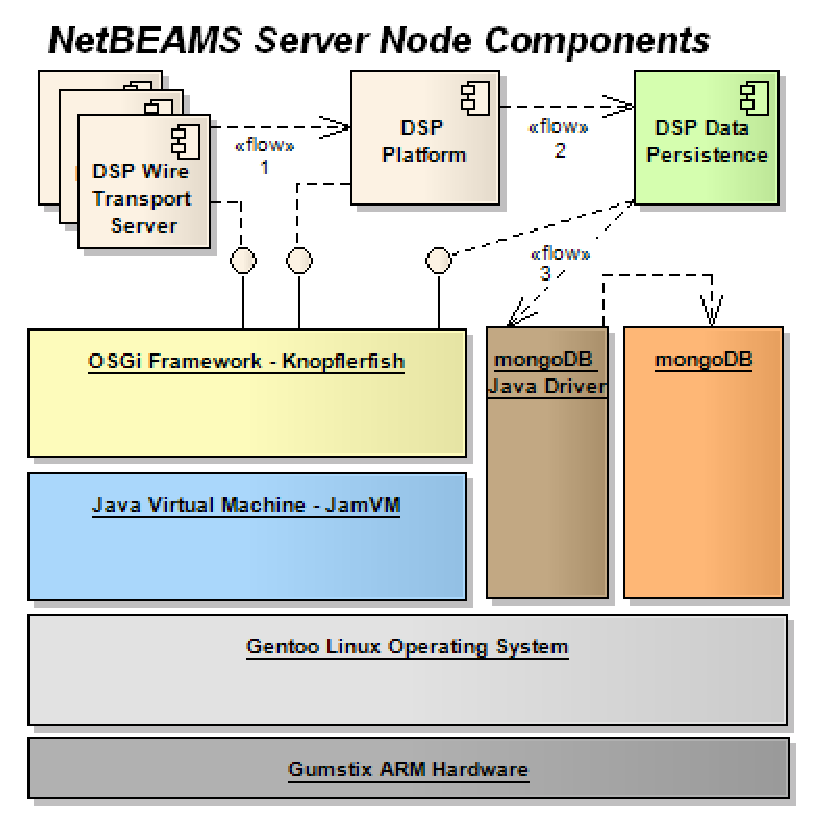
\includegraphics[scale=0.5]{../diagrams/NetBEAMS-Persistence-Server-Node-Components}
  \caption{UML Components diagram of the DSP Data Collector}
  \label{fig:NetBEAMS-Persistence-Server-Node-Components}
\end{figure}

As it is depicted on image 3.4.1, the DSP Data Persistence component can be
added into the system as an independent plug-and-play component. In addition,
the database system and the necessary drivers are also added without any
changes to the existing DSP infrastructure. First, as DSP Messages are
delivered to the server through the DSP Wire Transport Server, as shown by flow
1, the DSP Platform is responsible to forward a copy of the Measurement
messages directly to the DSP Data Persistence as shown by flow 2. Then, the
sole responsibility of the DSP Data Persistence is to transfer the received
measurement messages to the database system by using the connection drivers, as
depicted by flow 3.

The following sections focus on the DSP Data Persistence component design, and
in this way, any references to the DSP Platform can be seen on section 2.4.

\section{DSP Data Persistence: OSGi-DSP Bundle Design}

The new proposed Data Persistence component must follow the DSP requirements
for a new DSP Component. As described on section 2.4, any DSP component follows
the design-pattern of Data Producer/Consumer. Similarly, section 3.2 described
the requirements that the DSP Data Persistence must handle, taking into account
the data model and database connection.

After reviewing the requirements of section 3.2, the resulting model maintains
the dependency among 4 different major Java packages. The addition of a DSP
Data Persistence component depends on 2 existing packages, namely the OSGi
Framework and the DSP Platform as in any DSP Component, and an additional
package for the database access driver API. The UML Package dependency diagram
of image 3.5.x shows these dependencies, which are used to better track changes
among the packages.

\begin{figure}[!h]
  \centering
  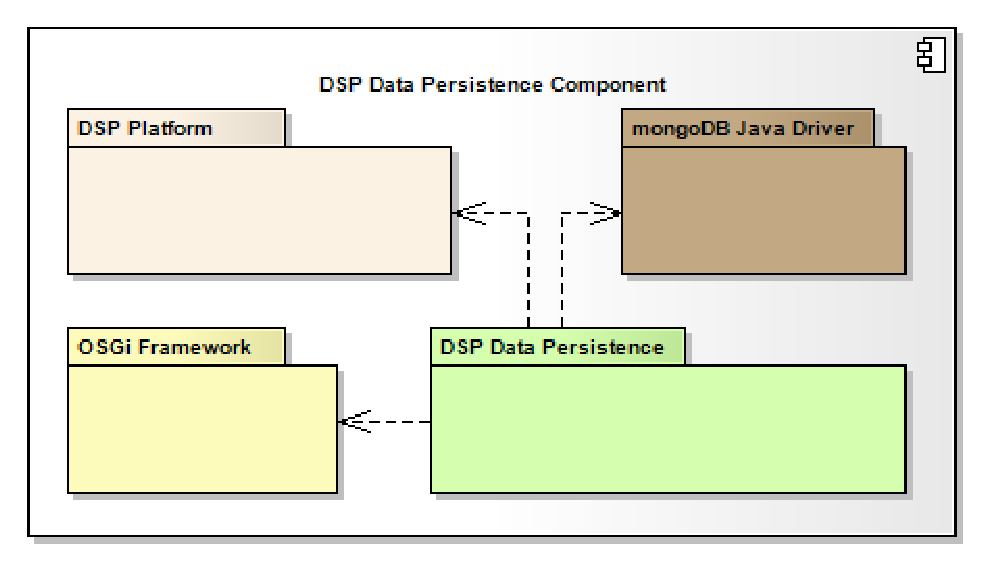
\includegraphics[scale=0.5]{../diagrams/DSP-Data-Persistence-Packages-Dependency}
  \caption{UML Components diagram of the DSP Data Collector}
  \label{fig:DSP-Data-Persistence-Packages-Dependency}
\end{figure}

The following sections details each step of the DSP Data Persistence activation
and parallel execution of the contained classes.

\subsection{DSP Data Persistence Activation and Message Delivery}

As shown on section 2.4.3, the DSP Platform is composed of loosely-coupled
components. In this way, this section describes the addition of the DSP Data
Persistence, as shown on the UML Class diagram of image 3.5.1.1.

\begin{figure}[!h]
  \centering
  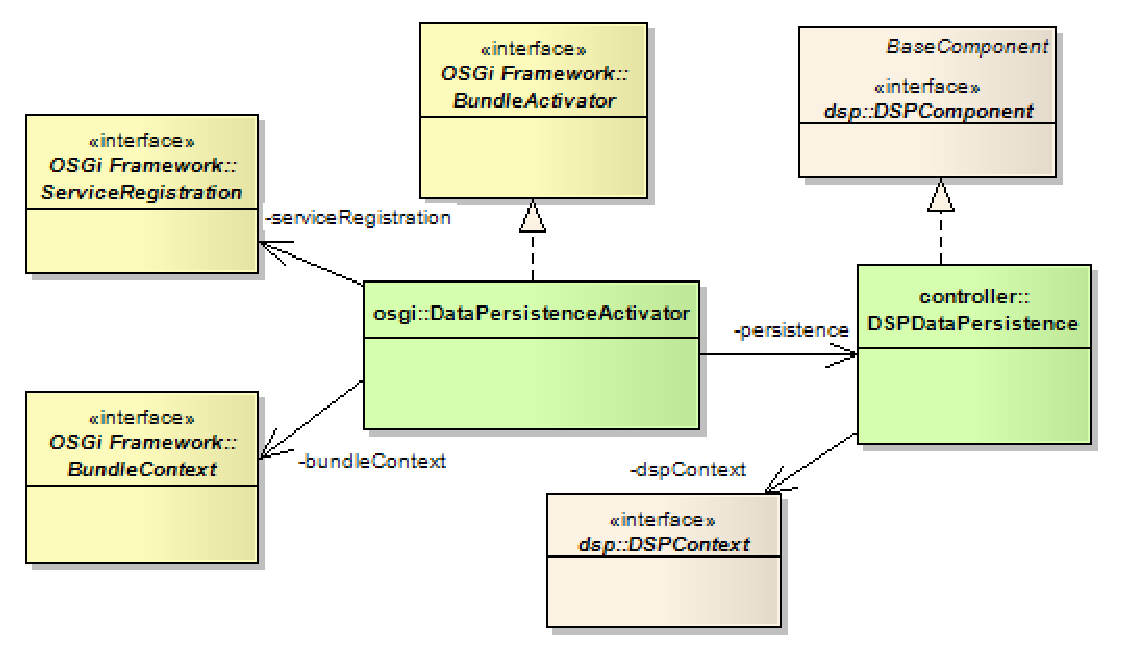
\includegraphics[scale=0.5]{../diagrams/DSP-DataPersistence-Activator-Class-Diagram}
  \caption{UML Class diagram for the DSP Data Persistence Activator and Component}
  \label{fig:DSP-DataPersistence-Activator-Class-Diagram}
\end{figure}

The DSP Data Persistence Activator is the main class responsible for the
activation of the DSP Data Persistence component, as it extends the OSGi class
BundleActivator and maintains a reference of the DSP Data Persistence class.
Furthermore, the activator maintains references to the classes BundleContext
and ServiceReference both from the OSGi Framework. The former is responsible
for maintaining the link with the OSGi Framework, while the latter is used to
register the DSP Component as a service. Therefore, it is clear that the class
DSP Data Persistence Activator is the main communication interface between the
DSP Platform and the OSGi Framework.

While the DSP Data Persistence Activator is responsible for the orchestration
of the classes during the execution on the OSGi Framework, the class DSP Data
Persistence extends from the DSP Platform class DSPComponent. For this reason,
this class inherits all the behavior described on section 2.4 and can be in the
roles of Data Consumer and a Data Producer.

\begin{itemize}
  \item \textbf{DSP Data Persistence as Data Consumer}: receives any measurement
  message from remote sensors;
  \item \textbf{DSP Data Persistence as Data Producer}: transforms any
  measurement message received into a format that must be ready to be saved on the
  database, based on the description of the data model of section 3.3.
\end{itemize}

The DSP Data Persistence Activator follows the states described on the state
diagram of image 2.4.3.4, as it is an extension of the OSGI class
BundleActivator, as well as being responsible for stopping or starting the the
DSP Data Persistence component instance. As described on section 2.4, the
following steps must take place in order to activate and start the DSP Data
Persistence component, described partially on image 2.4.6.3:

\begin{enumerate}
  \item During the DSP Platform activation, it will get the name of the
  persistence component from the configuration artifact config.xml;
  \item After being selected based on the configuration priority, the DSP
  Bundle artifact is identified and installed, by creating an instance of the
  class DSP DataPersistence Activator and making a call to the method start(),
  as shown on image 3.5.1.2;
  \item During the activation, an instance of the DSP Data Persistence
  component is created and registered as an OSGi Service;
  \item Upon registering the DSP Data Persistence component, the DSP Platform
  "listens" the event serviceUpdate() and, and triggers the last operations to
  bootstrap the DSP Component:
   \begin{enumerate}
      \item Initializes the component by calling the method initComponent();
      \item Starts the component by calling the method startComponent();
      \item Bootstrap messages are delivered to the component.
   \end{enumerate}
\end{enumerate}

As the requirements defined on section 3.2 specifies the update of the DSP
Component during its initialization, an optional DSP Update Message will be
sent to the component during its initialization process, as described on
section 2.4. The initialization of the DSP Component Activator and the DSP
Component registration are shown on image 3.5.1.2.

\begin{figure}[!b]
  \centering
  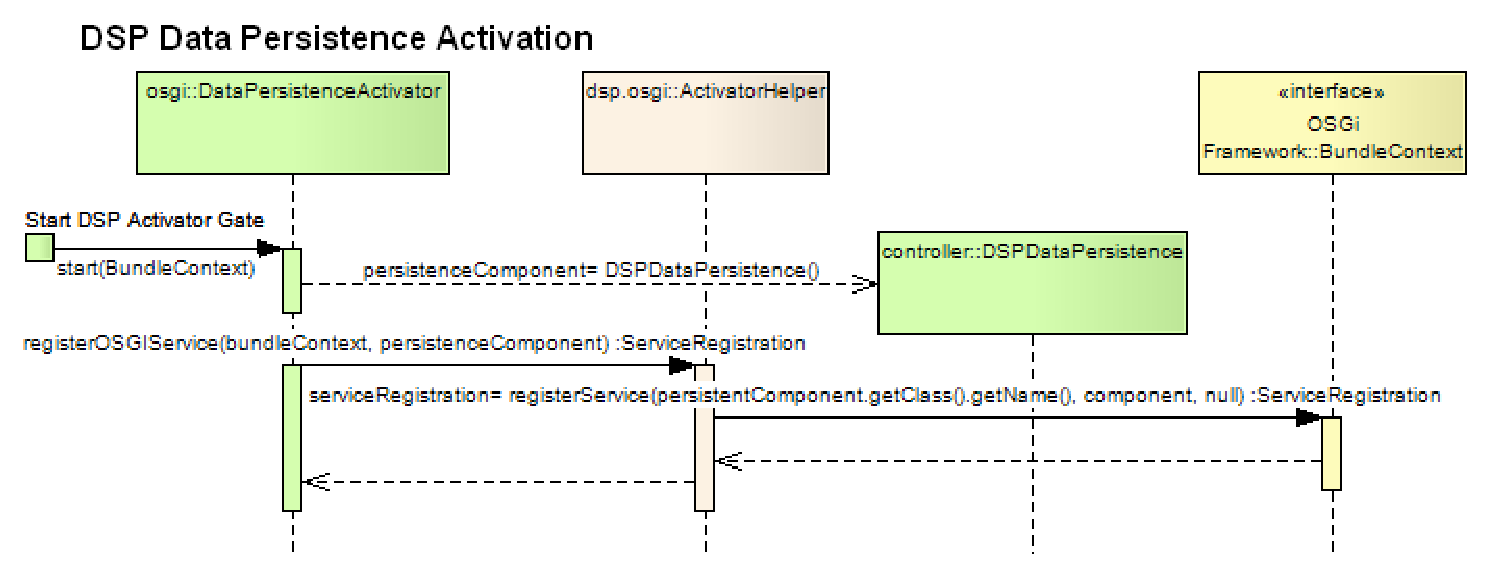
\includegraphics[scale=0.5]{../diagrams/From-OSGi-Framework-to-DSP-Data-PersistenceActivator-Sequence-Diagram}
  \caption{UML Sequence diagram describing the DSP Data Persistence bundle activation}
  \label{fig:From-OSGi-Framework-to-DSP-Data-PersistenceActivator-Sequence-Diagram}
\end{figure}

The the gate "Start DSP Activator Gate" reaches the DSP Data Persistence, it
first creates the unique instance of the class DSP Data Persisence and uses
that instance to register it as the OSGi service through the call to the DSP
Platform helper class ActivatorHelper. At this point, the DSP Data Persistence
has been installed and is in the state "Active".

\subsection{Delivering Bootstrap and Measurement Messages}

Although the DSP Data Persistence component has been instantiated as of image
3.5.1.2, the process of delivering messages to the DSP Data Persistence has yet
to be completed. As defined by the requirements, the DSP Component must execute
its function in a concurrent fashion, using configuration parameters during its
bootstrap process. The class DSP Data Flusher is responsible for running as a
"worker thread", whose function is to verify if there are messages to be
flushed into the Database with the class Transient Persistence Layer. Image
3.5.2.1 describes the remaining UML Class diagram for the main classes of this
functionality.

\begin{figure}[!b]
  \centering
  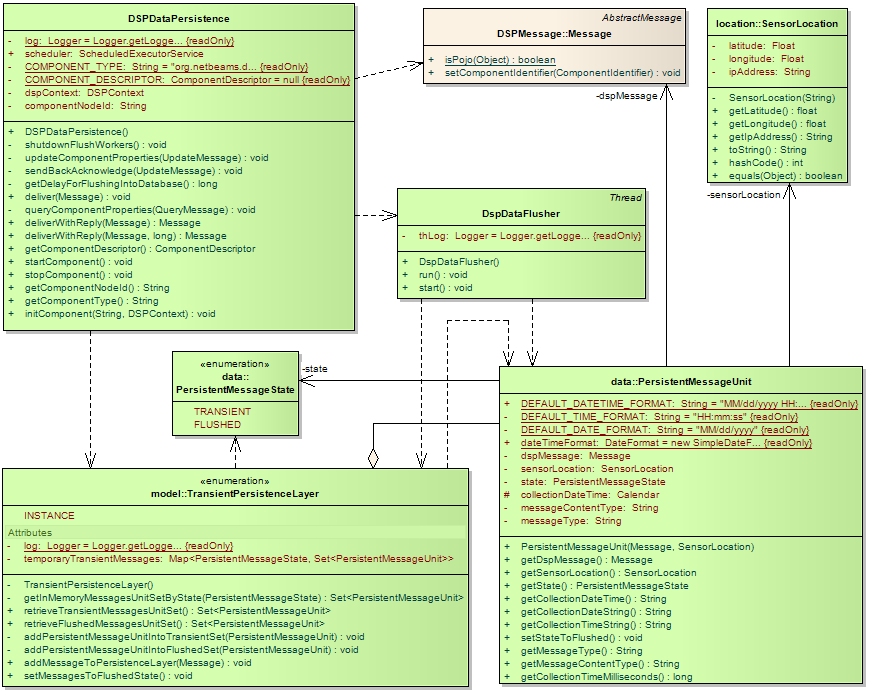
\includegraphics[scale=0.5]{../diagrams/DSP-DataPersistence-Flusher-Classes}
  \caption{UML Class diagram with the DSP Data Flusher worker thread}
  \label{fig:DSP-DataPersistence-Flusher-Classes}
\end{figure}

The DSP Data Flusher is a thread that is designed to be in two different
states: RUNNABLE and TIMED\underline{ }WAITING. In the former, the DSP Data Flusher will be
contacting the Transient Persistence Layer to verify if there are any message
waiting to be sent to the Database service, while in the latter the DSP Data
flusher will be waiting for the next cycle defined by the bootstrap parameter
TRANSIENT\underline{ }DATA\underline{ }FLUSHER\underline{ }DELAY.


\begin{figure}[!b]
  \centering
  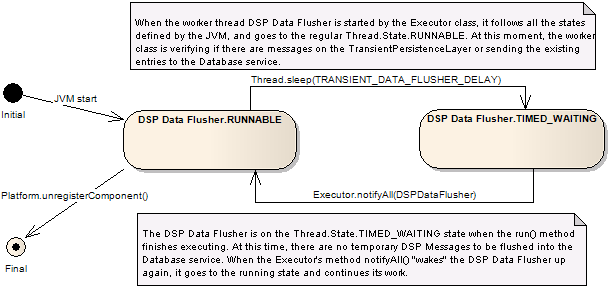
\includegraphics[scale=0.5]{../diagrams/DSP-DataPersistence-Flusher-State-Diagram}
  \caption{UML State diagram for the DSP Data Flusher Worker Thread}
  \label{fig:DSP-DataPersistence-Flusher-State-Diagram}
\end{figure}

Upon receiving a new DSP measurement message, the DSP Data Persistence
component must send its reference to the temporary memory space, as described
by the non-functional requirement on section 3.2. In this way, the DSP Data
Persistence component maintains a dependency on the Singleton class
TransientPersistenceLayer, which is responsible for keeping track of messages
that are received by working component. However, in order to add the DSP
message into its aggregated map, it first transforms the message into an
instance of the class PersistentMessageUnit, which has references to the class
regarding the location of the message,  SensorLocation.

The last paragraph of section 2.4.7 described the last steps of the Sequence
Diagram regarding DSP Message delivery to the DSP Broker on the DSP Server
host. For this reason, Image 3.4.1.2 continues the steps of the DSP Broker from
the gate "From DSP WireTransport Server to Broker Gate", showing the steps
taken to transfer a DSP Message to the Singleton class
TransientPersistenceLayer.

According to the DSP Broker model described on section 2.4.6, the DSP Matcher
needs to be updated with the addition of a matching rule that filters a copy of
any Measurement Message (section 2.4.4) to the DSP Data Persistence component
designed. As it is shown in figure
\ref{fig:From-DSP-Broker-To-DSPDataPersistence-General-Sequence}, the worker
Thread DSP Data Flusher is the link between the Transient and Persistent
layers, as it depends on the references from the classes
TransientPersistenceLayer and the DSPMongoCRUDService. The former maintains
DSP Messages in memory wrapped by an instance of PersistenceMessageUnit and
the latter is responsible for sending the MessageContent from the DSPMessage
body to the Database.

\begin{figure}[!b]
  \centering
  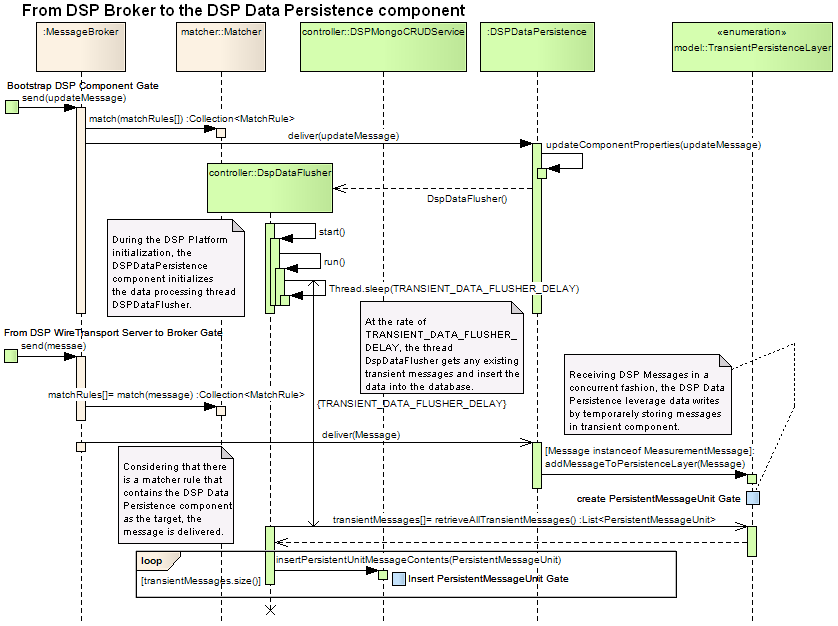
\includegraphics[scale=0.5]{../diagrams/From-DSP-Broker-To-DSPDataPersistence-General-Sequence}
  \caption{UML Sequence Diagram - Flow 1: From the DSP Broker to the Data
  Persistence Component}
  \label{fig:From-DSP-Broker-To-DSPDataPersistence-General-Sequence}
\end{figure}

The DSP Broker retrieves the list of matching rules by contacting the Matcher.
As the DSP Platform have already loaded all the Matching rules, a copy of a
given DSP message is delivered to the DSP Data Persistence component. However,
the sequence diagram shows two different stages of reception:

\begin{itemize}
  \item A bootstrap DSP Update Message is delivered to the DSP Data Persistence
  component when the DSP Platform is initializing the component. In this way,
  the DSP Data Persistence can initialize the DspDataFlusher worker thread to
  flush temporary messages into the database at the rate of
  TRANSIENT\underline{ }DATA\underline{ }FLUSHER\underline{ }DELAY in seconds;
  \item Any DSP Measure Message can be persisted by the DSP Data Persistence
  component. When the DSP Broker delivers a DSP MeasureMessage to this
  component, it will add the message to a temporary memory location to decrease
  I/O on the database, as depicted by the gate "create PersistentMessageUnit
  Gate". The simple procedure to add the message into the transient persistent
  layer is shown on image 3.4.3.
\end{itemize}

The class PersistenceMessageUnit is the major transient persistence unit that
carries references regarding the originating DSP Message that was collected by
the DSP Data Persistence component. It is composed by a SensorLocation and
contains a reference to the PersistentMessageState enumaration. The former
identifies which sensor produced the collected data from the DSP Message by the
IP address, while the latter identifies whether the PersistenceMessageUnit has
been saved into the Database or not as depicted by the UML State diagram in
figure \ref{fig:PersistentMessageState-Diagram}.

\begin{figure}[!b]
  \centering
  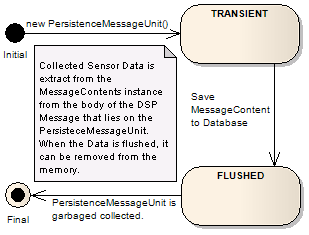
\includegraphics[scale=0.5]{../diagrams/PersistentMessageState-Diagram}
  \caption{UML State Diagram for the instance of the class
  PersistentMessageState}
  \label{fig:PersistentMessageState-Diagram}
\end{figure}

\begin{figure}[!b]
  \centering
  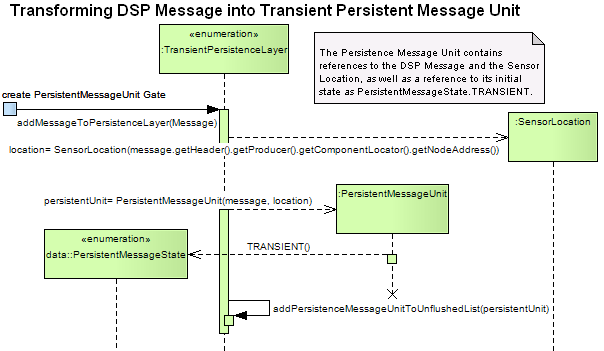
\includegraphics[scale=0.5]{../diagrams/From-Create-PersistentMessageUnit-to-TransientPersistence-Layer-Sequence}
  \caption{UML Sequence diagram - Adding a DSP Message into the Transient Persistence layer}
  \label{fig:From-Create-PersistentMessageUnit-to-TransientPersistence-Layer-Sequence}
\end{figure}

According to section 3.4.1, the persistence model must carry information
regarding which sensor device produced the collected data. For this reason, an
instance of the class SensorLocation carries the information about the IP
address from the component that originally produced the DSP Message. Then, an
instance of the class PersistenceMessageUnit is created, having its state on
TRANSIENT, as detailed on UML State diagram on Image 3.4.2.

\subsection{Flushing data into the Database}

The last stage sequence described on the Sequence diagram of Image 3.4.3
depicts the DspDataFlusher worker thread continuously waking up at the rate of
TRANSIENT\underline{ }DATA\underline{ }FLUSHER\underline{ }DELAY. Its purpose is as simple as to iterate over the
list of PersitenceMessageUnit on the state of TRANSIENT, and send each of them
to be saved on the persistence storage. Figure
\ref{fig:DSP-Data-Persistence-Classes} shows the participating classes of the
component.

\begin{figure}[!b]
  \centering
  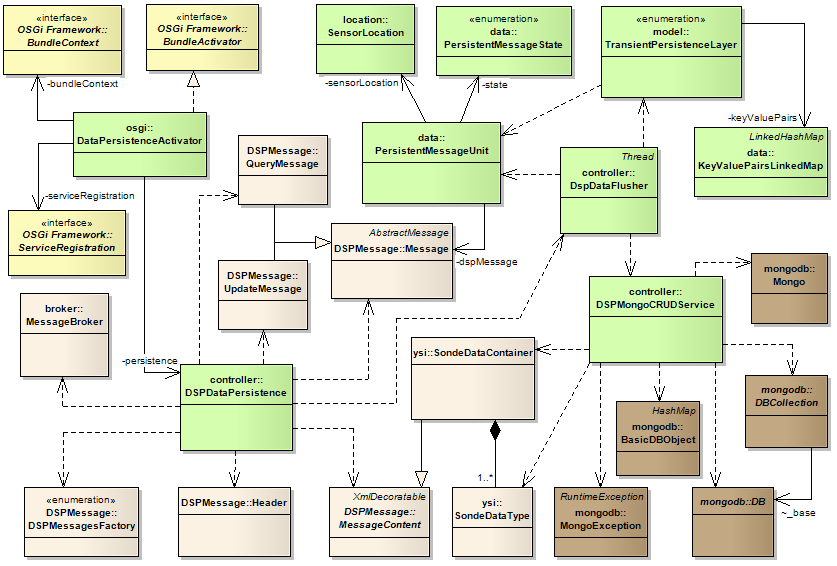
\includegraphics[scale=0.5]{../diagrams/DSP-Data-Persistence-Classes}
  \caption{UML Class diagram for the DSP Data Persistence component.}
  \label{fig:DSP-Data-Persistence-Classes}
\end{figure}

Finally, this sequence of events is continued by the "insert
PersistenceMessageUnit Gate", which triggers the persistence service from the
chosen database system as shown on Image 3.4.5.

\begin{figure}[!b]
  \centering
  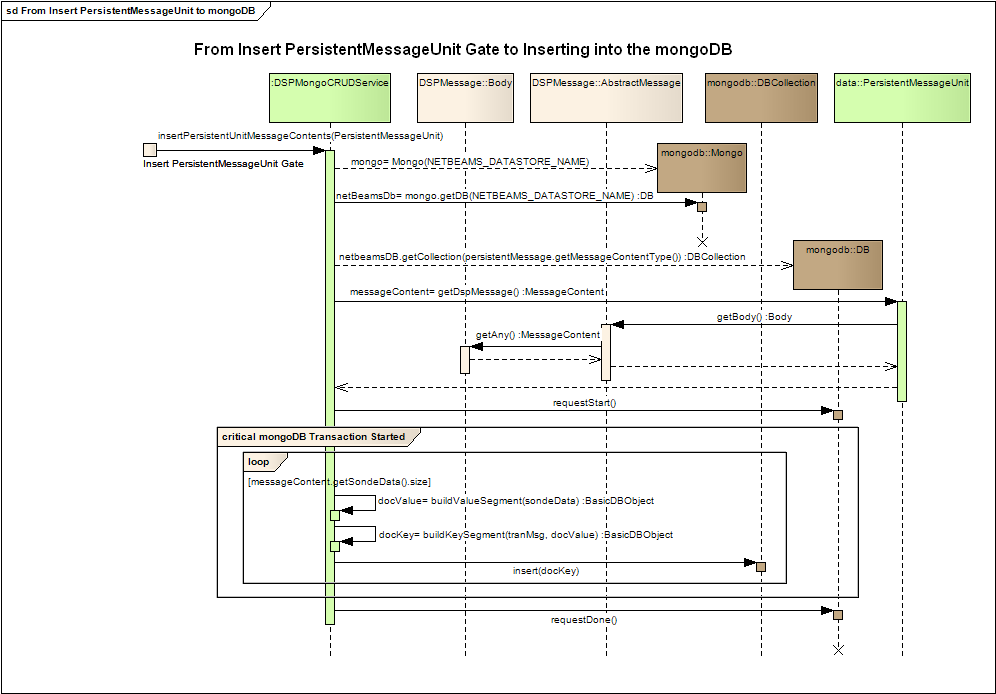
\includegraphics[scale=0.5]{../diagrams/From-Insert-PersistentMessageUnit-to-mongoDB}
  \caption{UML Sequence Diagram - MessageContent instance saved by the class
  mongoDB service}
  \label{fig:From-Insert-PersistentMessageUnit-to-mongoDB}
\end{figure}

In order to build the document key and value segments as described on section
3.2. First, the value is built by extracting the DSP Message Content from the
body of the DSP Message.

\begin{figure}[!b]
  \centering
  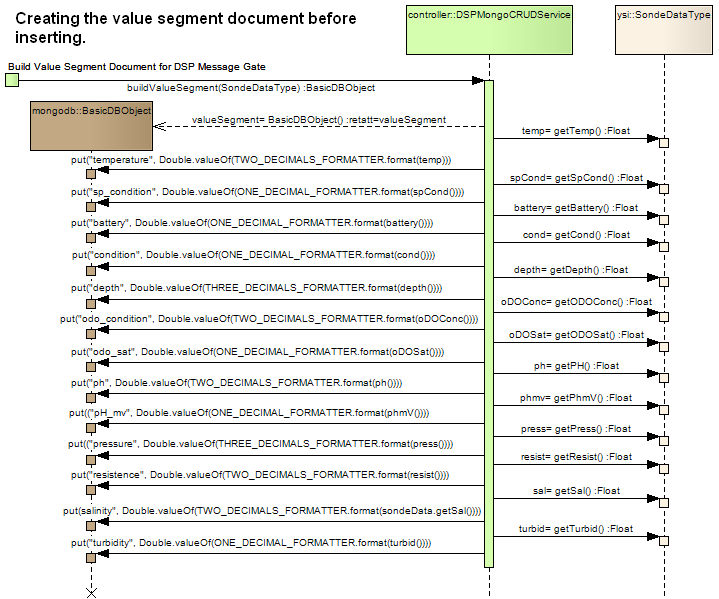
\includegraphics[scale=0.5]{../diagrams/From-Creating-Value-Segment-Sequence}
  \caption{UML Sequence diagram showing the creation of the value document segment}
  \label{fig:From-Creating-Value-Segment-Sequence}
\end{figure}

Finally, the document key segment is prepared as follows on image 3.4.7.

\begin{figure}[!b]
  \centering
  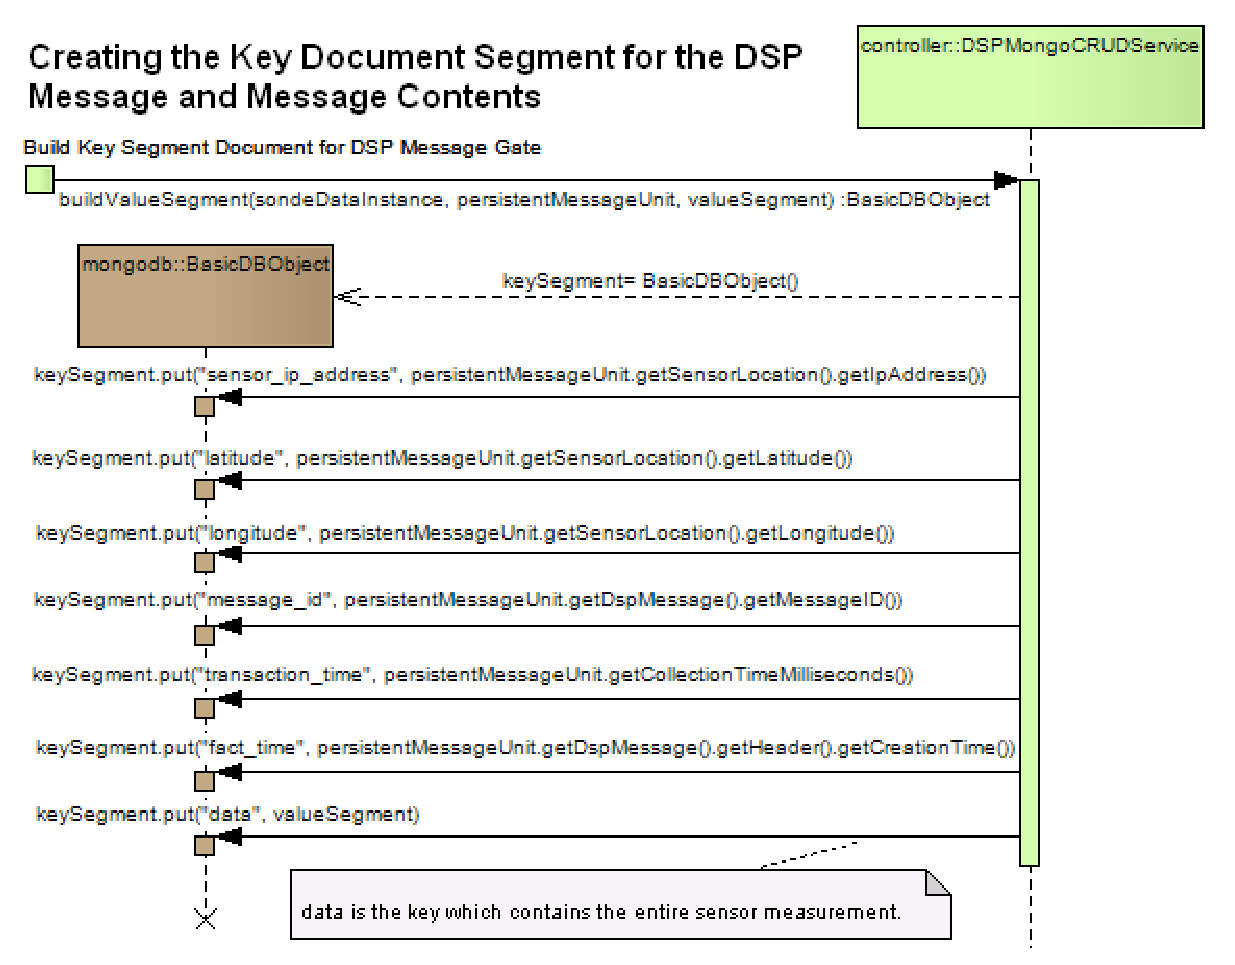
\includegraphics[scale=0.5]{../diagrams/From-Creating-Key-Segment-Sequence}
  \caption{UML Sequence diagram showing the creation of the key document segment}
  \label{fig:From-Creating-Key-Segment-Sequence}
\end{figure}







\subsection{DSP Data Persistence Implementation}

This section shows the implementation of the DSP Data Persistence, which
follows the specifications of the DSP Components described on section 2.4,
along with the setup of the mongoDB, the chosen database system that handles
document-oriented instances. The implementation of the DSP Data Persistence
component was developed using the DSP Subversion repository at
http://code.google.com/p/netbeams.

The Deployment diagram with a single host, single database;
Deployment diagram with single host, multiple shards;
Deployment diagram with dedicated database host, single database;
Deployment diagram with dedicated cluster host, multiple shards/replicas;

Each of the deployment schema have two different deployment components: the DSP
component deployment and the database instance installation and configuration.
The following section shows each of the components artifacts and configuration
necessary.

\subsubsection{DSP Deployment on OSGi Framework}

    * Description of the OSGi MANIFEST.MF
    * Description of the component on the config.xml
    * Adding a matching rule on the matcher\underline{ }config.xml
    * Adding a bootstrap message the component and database configuration


    * Adding a new entry into the deployment configuration artifact config.xml;
    * Adding a new entry into the matcher configuration artifact matcher\underline{ }config.xml;
    * Adding an optional configuration message that sets up the new DSP Component;
    * Adding new Java drivers that communicates with the Database system;
    * Installing and configuring the proposed database system.
%% main.tex, to be used with thesis.tex
% This contains the main work of your thesis.

%\bibliography{thesis}  % uses the references stored in Chapter1Radar.bib

\chapter{DSP Data Persistence: Component Implementation}

This section shows the implementation of the DSP Data Persistence, which
follows the specifications of the DSP Components in the previous chapter,
along with the setup of the mongoDB, the chosen database system that models
data in a type of key-value pair model. Moreover, this chapter also describes
the experiments conducted for the persistence.

The implementation of the DSP Data Persistence component, as well as the
implementation of the experiments, were developed and managed using the DSP a
reserved development branch at the Subversion \cite{subversion} repository
located at the Google Code website. In this way, anyone can checkout the entire
source-code from the branch
\textit{https://netbeams.googlecode.com/svn/branches/marcello/persistence},
as shown in Figure \ref{fig:dsp-data-persistence-dir}. In this way, the
recommended checkout branch directory will give the remaining directory
structure as summarized:

\begin{itemize}
  \item \textbf{NEBEAMS-DIR/}: the directories under the subdirectory
  ``persistence'';
  \item \textbf{DEV-VERSION}: the directory of the current development
  version for the DSP; That is, ``\textbf{NEBEAMS-DIR}/versions/v2/''
  \item \textbf{PERSISTENCE-DIR}: the directory of the DSP component, that is,
  ``\textbf{DEV-VERSION}/apps/osgi-intro-bundles/dsp/DSPDataPersistence''.
\end{itemize}

\begin{figure}[!b]
  \centering
  \includegraphics[scale=0.6]{../diagrams/dsp-data-persistence-dir}
  \caption{The DSP Data Persistence Directory Structure}
  \label{fig:dsp-data-persistence-dir}
\end{figure}

The DSP Platform defines its own run-time directory, which organizes the
artifacts used by the osgi-intro Framework, as well as the its own configuration
descriptor and matcher, as described in the previous section. 

\begin{itemize}
  \item \textbf{RUNTIME-DIR}: the main directory for the execution of the DSP
Platform, with all the necessary osgi-intro-related artifacts are placed, as shown in
Figure \ref{fig:dsp-runtime-dir}.
\end{itemize}

\begin{figure}[!t]
  \centering
  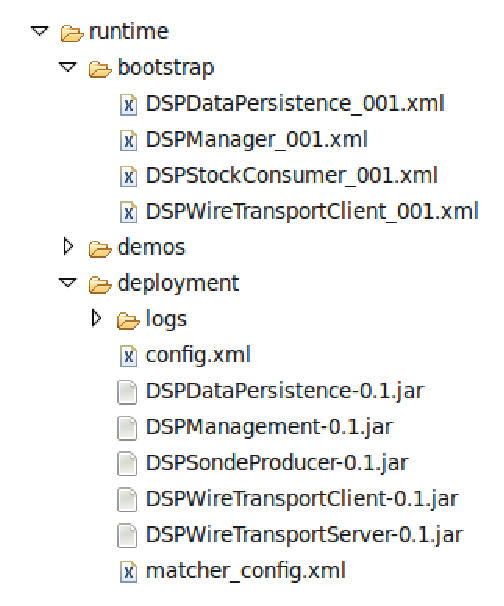
\includegraphics[scale=0.5]{../diagrams/dsp-runtime-dir}
  \caption{The DSP Data Persistence Directory Structure}
  \label{fig:dsp-runtime-dir}
\end{figure}

\section{DSP Platform Deployment}

As described in the previous chapter, the DSP Data Persistence Component was
implemented using the Java Programming language, on top of the osgi-intro Framework
API. This section describes the setup process of the implementation, as well as
the artifacts use during the implementation, which will be listed in the
appendix section.

The structure of the artifacts implemented for the DSP Data Persistence
Component follow the conventions of the NetBEAMS implementation, where the main
directory \textbf{PERSISTENCE-DIR}, depicted by Figure
\ref{fig:dsp-data-persistence-dir-checkedout}, holds each of the development
artifacts.

\begin{itemize}
  \item \textbf{DSPDataPersistence}: Main directory with the build.xml (Listing
  \ref{file:dsp-build.xml}) and other Eclipse-related artifacts. The other
  major directories are also listed:
  \item \textbf{META-INF}: this directory contains the descriptor file for
  the osgi-intro Framework, this this case the MANIFEST.MF;
  \item \textbf{src}: the main directory structure for the source-code
  implemented. Note that it follows the Java specification for packaging, and
  therefore, lists the package org.netbeams.dsp.persistence as the main
  package, including the layers controller, model and osgi-intro.
\end{itemize}

\begin{figure}[!h]
  \centering
  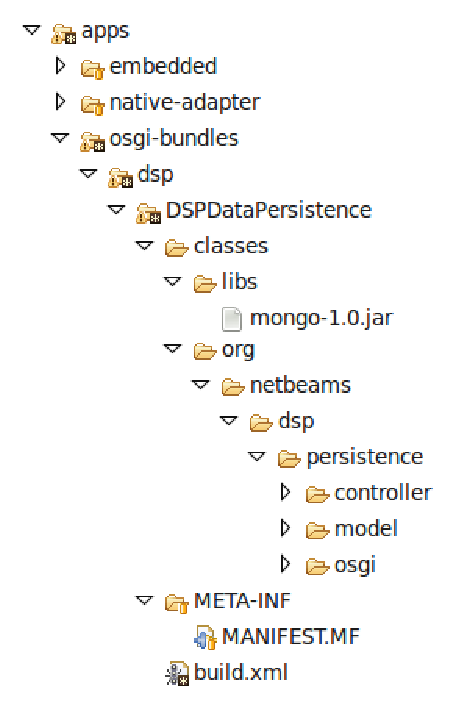
\includegraphics[scale=0.5]{../diagrams/dsp-data-persistence-dir-checkedout}
  \caption{The DSP Data Persistence Directory Structure}
  \label{fig:dsp-data-persistence-dir-checkedout}
\end{figure}

\subsection{osgi-intro Deployment Process}

Since each NetBEAMS component is managed by an osgi-intro component and its
infrastructure, this section describes the basic functionality of the osgi-intro
platform \cite{osgi-intro}, a framework was conceived to support modularity in
terms resources-limited environments such mobile devices and vehicles, but it
was first widely deployed on Eclipe IDE\footnote{Integrated Development
Environment}, because it promotes the use of reusable loosely-coupled modules
using the Java Programming Language \cite{java}. The most basic layer of the
osgi-intro Framework depicted in Figure \ref{fig:layering-osgi-intro} are as follows:

\begin{itemize}
  \item \textbf{Module Layer}: manages the osgi-intro bundles deployed on the osgi-intro
  Platform, providing the necessary "wiring" of the components. In other words,
  the modules, called osgi-intro Bundles, can export and/or import packages in the
  level of a Java Class managed by the osgi-intro Framework;
  \item \textbf{Service Layer}: resposible for the interoperability between 2
  or more bundles, enabling the bundles to register services offered by
  the its specification;
  \item \textbf{Execution Layer}: executes the bundles, managing and changing
  their life-cycle through the bundle execution.
\end{itemize}

\begin{figure}[!h]
  \centering
  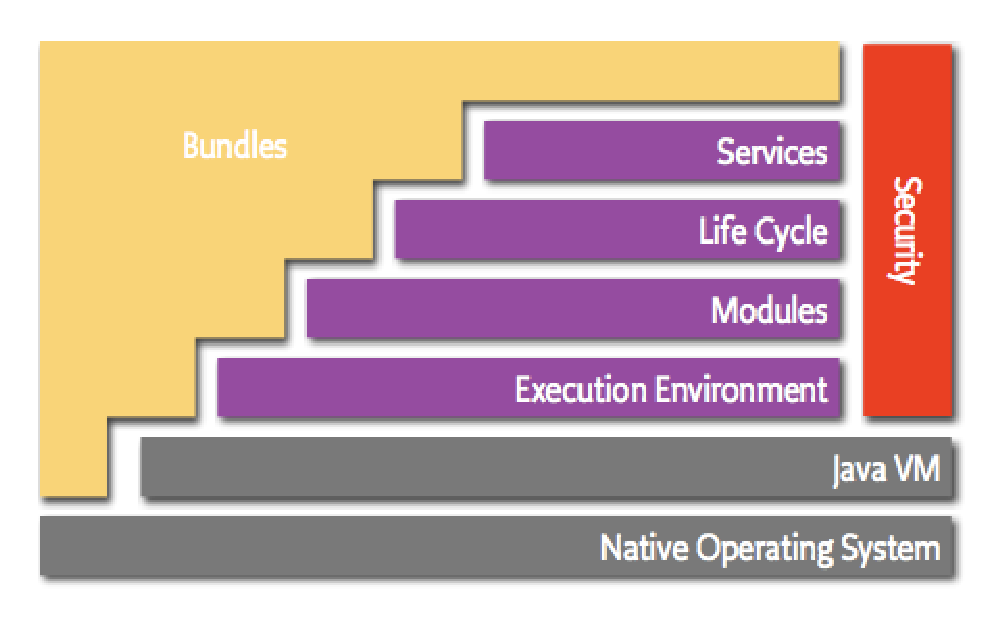
\includegraphics[scale=0.5]{../diagrams/layering-osgi}
  \caption{The osgi-intro Framework Layers}
  \label{fig:layering-osgi-intro}
\end{figure}

NetBEAMS uses the concept of the modularization through the use of the the
Producer-Consumer paradigm described in the previous section. Since the DSP
Components are essentially osgi-intro bundles, the interoperability between them are
given in the implementation and reuse existing bundles in the osgi-intro Framework
and the DSP Platform, described by an artifact called MANIFEST.MF as seen in
listing \cite{file:osgi-intro-manifest}. In general, an osgi-intro bundle must
provide specifications that describes the module to be published into the osgi-intro
Framework. In this way, the main properties of the osgi-intro MANIFEST.MF artifact can
used by the DSP Data Persistence can be summarized as follows:

\begin{itemize}
  \item \textbf{Bundle-Activator}: The name of the instance of an osgi-intro Activator
  class, responsible to manage the bundle. The implemented class
  ``DataPersistenceActivator'' provides the activation mechanisms for the
  services provided by the DSP Data Persistence Component;
  \item \textbf{Bundle-ClassPath}: the necessary Java Jars list needed to run
  the bundle. It lists the mongoDB Java driver as one of the required
  dependencies deployed in the same package;
  \item \textbf{Import-Package}: the Java Packages needed by the DSP Data
  Persistence Component Bundle. These Java Packages must be provided by other
  DSP components, forcing the execution to be dependent on those package.
  They are provided through a ``Export-Package'' section in other osgi-intro
  bundles and, as it is shown in listing \cite{file:osgi-intro-manifest}, they
  are from different packages.
\end{itemize}

Once the osgi-intro bundle is installed into the osgi-intro Platform, it will be managed by
the osgi-intro Execution layer and change the bundle state according to its
lify-cycle, as described in the previous chapter. Therefore, the packaging of
the osgi-intro source-code is done using a JAR\footnote{Java Archival Repository}
artifact specification \cite{java-tutorial}. In this way, the DSP Data
Platform osgi-intro bundle JAR is created by the Apache ANT build script
\cite{apache-ant} in Listing \ref{file:dsp-build.xml}. The task
``dsp-data-persistence.all'' compiles all the source-code created from the
design of the previous chapter and packages everything into the artifact
``DSPDataPersistence-x.x.jar'', where x.x is the version of the bundle. Figure
\ref{fig:dsp-runtime-dir} shows the DSP Data Persistence file under the
dirctory ``\textbf{RUNTIME-DIR}/deployment/''.

\subsection{Adding DSP Data Persistence into DSP Platform }

Once the new component was developed, the DSP Data Persistence component was
deployed by editing two main descriptors, as well as the optional bootstrap
message, as described in chapter 5:

\begin{itemize}
  \item \textbf{config.xml}: the DSP Data Persistence is added to the DSP
  Platform adding an entry for the component;
  \item \textbf{matcher\underline{ }config.xml}: the addition of the rules that
  filters the messages to the DSP Data Persistence;
  \item \textbf{DSPDataPersistence\underline{ }001.xml}: depicts the bootstrap
  message for the DSP Data Persistence Component, as shown in Listing 
  \ref{file:dsp-data-pers-bootstrap.xml}.
\end{itemize}

The first configuration artifact enables NetBEAMS to initialize contain the
descriptor of the component, as shown in Listing \ref{file:dsp-config.xml}.
The component is added with the highest priority, since it contains
dependencies to other DSP Components. 
\subsection{Starting the DSP Platform}

Once the DSP Platform automatically installs all the components described by
the configuration descriptor, the container verifies the dependencies and
starts each of the DSP components of Figure \ref{fig:knopflerfish-execution},
the osgi-intro Framework container Knopflerfish \cite{knopflerfish}.

\begin{figure}[!t]
  \centering
  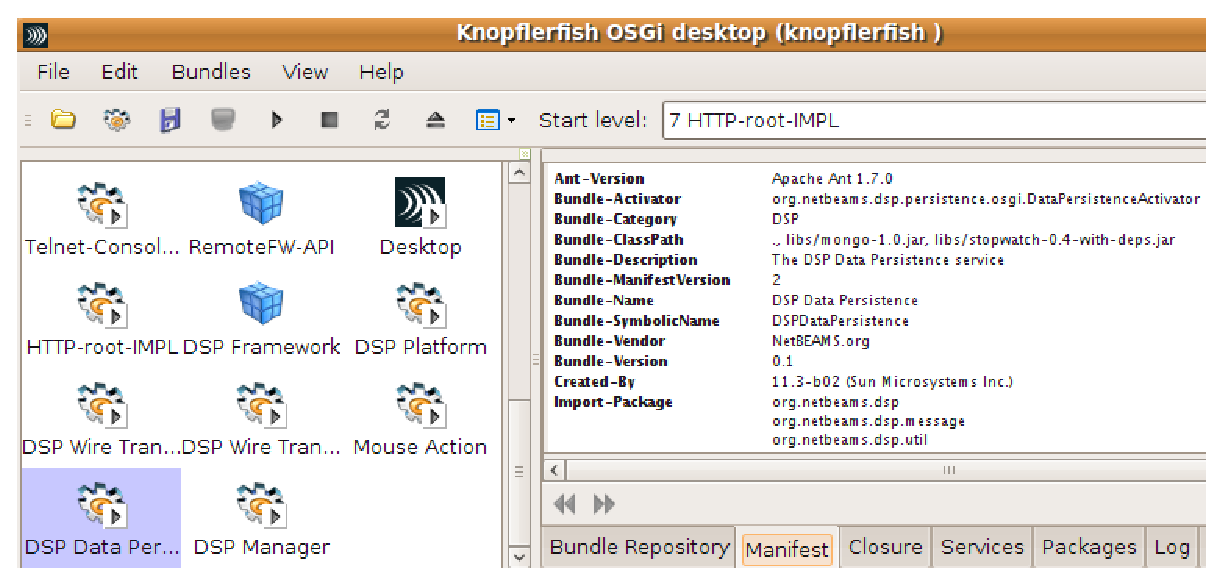
\includegraphics[scale=0.65]{../diagrams/knopflerfish-execution}
  \caption{The execution of the Knopflerfish Container}
  \label{fig:knopflerfish-execution}
\end{figure}

\subsection{Execution Logs}

\section{mongoDB Deployment}

Given that Document-Oriented Model makes a good candidate persist sensors'
properties and the recently enumerated list technologies in the previous
article DSPDataPersistence, the open-source project called mongoDB was chosen
for the evaluation on our case study, the netBEAMS DSP Platform.

mongoDB supports storage based on collections of data, stored using BSON, a
binary representation the JSON data representation format, including dynamic
queries and indexing support. As it's stated in their web site, mongoDB
"bridges the gap between key/value stores (which are fast and highly scalable)
and traditional RDBMS systems (which are deep in functionality)".

\begin{itemize}
  \item mongoDB implements a document-oriented structure, which is similar to
  KVP;
  \item mongoDB is written in C++, and therefore, can is available in any major
  platform, as well as offers a broad range of API drivers written in different
  languages such as Java, Python, Perl and Ruby; 
  \item mongoDB is open-source, with good community support and availability
  through mailing lists, freenode IRC channel, and commercial support through
  10gen company; 
  \item mongoDB has support to distributed systems properties such as
  Master-Slave replication, and features like Database Shards with
  auto-sharding based on shard keys.
\end{itemize}

The artifacts of the mongoDB are located in the thirdparty directory of the
NetBEAMS resources. However, the build script from the DSP Data Persistence
component can be executed to produce the persistence directory
structure for NetBEAMS, as described in figure
\ref{fig:dsp-persistence-system-dir}.

\begin{figure}[!h]
  \centering
  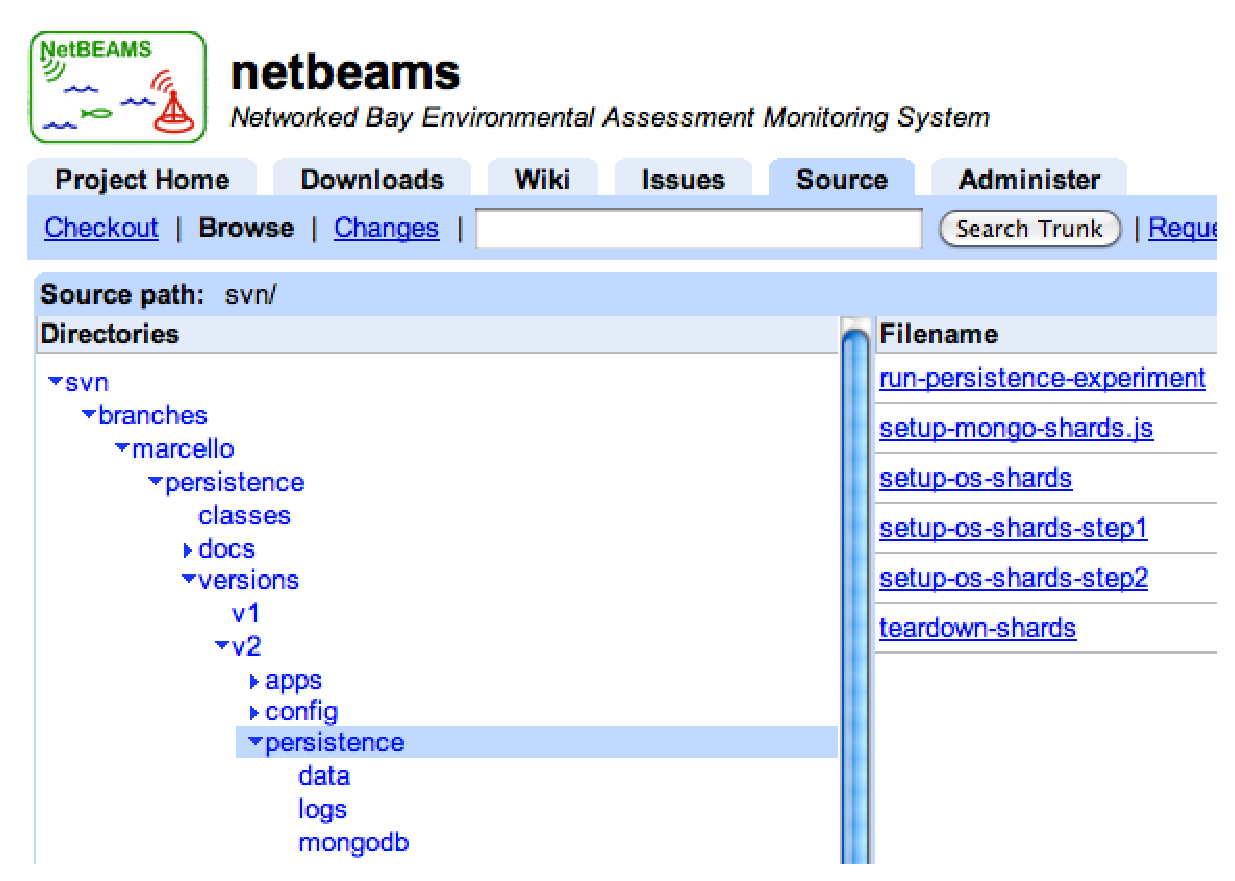
\includegraphics[scale=0.5]{../diagrams/dsp-persistence-system-dir}
  \caption{The osgi-intro Framework Layers}
  \label{fig:dsp-persistence-system-dir}
\end{figure}

Installation of mongoDB
- Explanation about mongoDB processes: mongod, mongos, mongo
- Specification of the shards, shard key, etc

    * The database instance is called "netbeams";
    * The database "netbeams" may contain different collections, categorized by
    the Sensor Content Type, that is, depending on how the DSP Component was
    described;  

\subsection{Document-Oriented Data Model}

An example of the data is as folows (using the JSON syntax). Listing
\ref{file:mongodb-ysi-data-format} follows the strategy described on Section X,
where the entity representation is denormalized, and each of the properties of
the sensor is repeated in each instance of the data. The fact and transaction
times are expressed in milliseconds. The data element contains the complete
structure of the originating sensor such as the IP address. The collection of
instances of this document represents the sensor data type.

\subsection{Starting the Database}

\subsection{Stopping the Database}

\subsection{Execution Logs}

- Java API implementation
- Python API implementation

\section{Data Access Using Database Shell}

The mongoDB client can be started by using the following command. Make sure you
have started the mongoDB server before executing the mongoDB client.

mongo netbeams | tee output\underline{ }number\underline{ }date.log

Here, the iterative mongo client shell offers users to verify and navigate on a
given database and its collections. This first section shows the connection of
the mongo client to the database netbeams. It also highlights the query for the
collections available. During the experiment, the SondeDataContainer?
collection was created as related to the type from the DSP Messages for the YSI
Sonde.

The shell references to the mongoDB system can be found at
http://www.mongodb.org/display/DOCS/dbshell+Reference 

\lstset{label=cmd:mongo,caption=Execution of mongo client}
\begin{lstlisting}
MongoDB shell version: 1.1.0-
url: netbeams
connecting to: netbeams
type "help" for help
> show collections
SondeDataContainer
system.indexes
>
> db.SondeDataContainer.count()
1000000
\end{lstlisting}

Then, the first verification of the data integrity is regarding the number of
elements created. Here, the first count() function on the collection returned
1000000.

An example about retrieving the first element of the collection can be done
using the findOne() function. It will return an element instance on the
JSONnotation.

\lstset{label=cmd:mongo-findone,caption=Querying the database: one item}
\begin{lstlisting}
> db.SondeDataContainer.findOne()
{
    "_id" : ObjectId("5d6f40078ec8074bba980900"),
    "message_id" : "020d82e1-18b2-4fe2-800c-a0f68e22ea86",
    "sensor" : {
        "ip_address" : "192.168.0.91",
        "location" : {
            "latitude" : 37.89155,
            "longitude" : -122.4464
        }
    },
    "time" : {
        "valid" : "Wed Nov 04 2009 02:30:12 GMT-0800 (PST)",
        "transaction" : "Sat Nov 21 2009 03:01:33 GMT-0800 (PST)"
    },
    "observation" : {
        "WaterTemperature" : 88.58,
        "SpecificConductivity" : 180.5,
        "Conductivity" : 167.3,
        "Resistivity" : 491.89,
        "Salinity" : 0.06,
        "Pressure" : 1.109,
        "Depth" : 2.642,
        "pH" : 7.11,
        "pHmV" : -42.9,
        "Turbidity" : 0.2,
        "ODOSaturation" : 72.4,
        "ODO" : 10.85,
        "Battery" : 2.7
    }
}
\end{lstlisting}

The query based on attributes can be done using the "dot" notation, as you
navigate through the JSON documents. Additionally, you can use the functions as
aggregated on the result of others. The example in listing
\ref{cmd:mongo-find-list} counts the number of documents with the key
"data.ph" equals to "5.64".

\lstset{label=cmd:mongo-find-list,caption=Execution of mongo client}
\begin{lstlisting}
> db.SondeDataContainer.find({"data.ph":5.64)}).count()
1226
\end{lstlisting}

The following example is the output of the first 2 documents from the same
previous query using the limit() function, as shown in figure
\ref{cmd:mongo-find-limit}.

\lstset{label=cmd:mongo-find-limit,caption=Query Element with specific
projection limiting the result set size}
\begin{lstlisting}
> db.SondeDataContainer.find({"data.ph":5.64}).limit(2)
{"_id" :  ObjectId( "d36f4007b7e7ac4a03c60000")  , "sensor_ip_address" : "192.168.0.136" , "message_id" : "7b6624d6-0ca1-4cba-a343-f166e88da73b"
, "transaction_time" : 1252845473412 , "fact_time" : 1252845346000 , "data" : {"temperature" : "45.01" , "sp_condition" : "37.6" ,
"condition" : "145.8" , "resistence" : "159.77" , "salinitude" : "0.0" , "pressure" : "0.391" , "depth" : "0.46" , "ph" : "5.64" ,
"pH_mv" : "-62.1" , "odo_sat" : "89.7" , "odo_condition" : "59.34" , "turbidity" : "0.0" , "battery" : "9.4"}}
{"_id" :  ObjectId( "d36f4007b7e7ac4a1fc80000")  , "sensor_ip_address" : "192.168.0.136" , "message_id" : "7b6624d6-0ca1-4cba-a343-f166e88da73b" ,
"transaction_time" : 1252845473412 , "fact_time" : 1252845346000 , "data" : {"temperature" : "46.71" , "sp_condition" : "60.8" ,
"condition" : "160.6" , "resistence" : "1399.4" , "salinitude" : "0.01" , "pressure" : "1.057" , "depth" : "2.485" , "ph" : "5.64" ,
"pH_mv" : "-16.3" , "odo_sat" : "58.8" , "odo_condition" : "19.29" , "turbidity" : "0.2" , "battery" : "9.2"}}
>
\end{lstlisting}

Other logs are located at
http://code.google.com/p/netbeams/downloads/list

\section{Data Access Using APIs}

The mongoDB server offers different drivers to access the data, as well as the
Web Services.

\begin{itemize}
  \item The Java tutorial on the drivers is located at
    http://www.mongodb.org/display/DOCS/Java+Tutorial. The driver is located on
    the NETBEAMS/versions/v2/thirdparty/mongodb directory;  
  \item The REST API can be called from any HTTP client. At the time of the
  editing, this feature is still under alpha version. Check the documentation
  athttp://www.mongodb.org/display/DOCS/Http+Interface for details 
\end{itemize}

The following HTTP GET Request method returns the first 5 documents in the collection:
http://127.0.0.1:28017/netbeams/SondeDataContainer/?limit=-5, as shown in
listing \ref{cmd:mongo-rest-request}.

\lstset{label=cmd:mongo-rest-request,caption=REST HTTP GET Request Example}
\begin{lstlisting}
HTTP/1.0 200 OK
x-action:
x-ns: netbeams.SondeDataContainer
Content-Type: text/plain;charset=utf-8

{
  "offset" : 0,
  "rows": [
    { "_id" : "156f4007e4c3b74a36ed3100", "sensor_ip_address" : "192.168.0.117", "message_id" : "08b02c08-9290-4517-9a28-c6ee7e16509a",
"transaction_time" : 1253557219486, "fact_time" : 1253557217000, "data" : { "temperature" : "31.44", "sp_condition" : "99.8", "condition" : "53.5",
"resistence" : "1157.08", "salinity" : "0.0", "pressure" : "1.066", "depth" : "0.161", "ph" : "1.08", "pH_mv" : "-82.0", "odo_sat" : "40.3",
"odo_condition" : "56.85", "turbidity" : "0.2", "battery" : "8.2" } } ,
    { "_id" : "156f4007e5c3b74a37ed3100", "sensor_ip_address" : "192.168.0.117", "message_id" : "08b02c08-9290-4517-9a28-c6ee7e16509a",
"transaction_time" : 1253557219486, "fact_time" : 1253557217000, "data" : { "temperature" : "37.83", "sp_condition" : "176.3", "condition" : "2.6",
"resistence" : "1324.97", "salinity" : "0.01", "pressure" : "1.36", "depth" : "1.564", "ph" : "0.12", "pH_mv" : "-23.5", "odo_sat" : "104.5",
"odo_condition" : "19.44", "turbidity" : "0.1", "battery" : "5.0" } } ,
    { "_id" : "156f4007e5c3b74a38ed3100", "sensor_ip_address" : "192.168.0.117", "message_id" : "08b02c08-9290-4517-9a28-c6ee7e16509a",
"transaction_time" : 1253557219486, "fact_time" : 1253557217000, "data" : { "temperature" : "74.3", "sp_condition" : "84.0", "condition" : "104.7",
"resistence" : "4089.13", "salinity" : "0.01", "pressure" : "1.222", "depth" : "2.788", "ph" : "6.56", "pH_mv" : "-78.1", "odo_sat" : "40.0",
"odo_condition" : "6.02", "turbidity" : "0.3", "battery" : "3.2" } },
  "total_rows" : 3 ,
  "query" : {} ,
  "millis" : 0
}
\end{lstlisting}

Data visualisation tools for mongoDB is slowly being developed by open-source
developers. The next picture shows the database "netbeams" and the collection
"SondeDataContainer  ?" being rendered by futon4mongodb, one of the
open-source tools developed to visualise mongoDB data.

\section{Visualizing Data on The Browser}

Futon4Mongo is an open-source software adapted from CouchDB \ref{couchdb}.
First, the collections list is shown. Figure
\ref{fig:view-collections-instance-browser-futondb} shows one single collection
for the YSI data containing 1 million objects.

\begin{figure}[h]
  \centering
  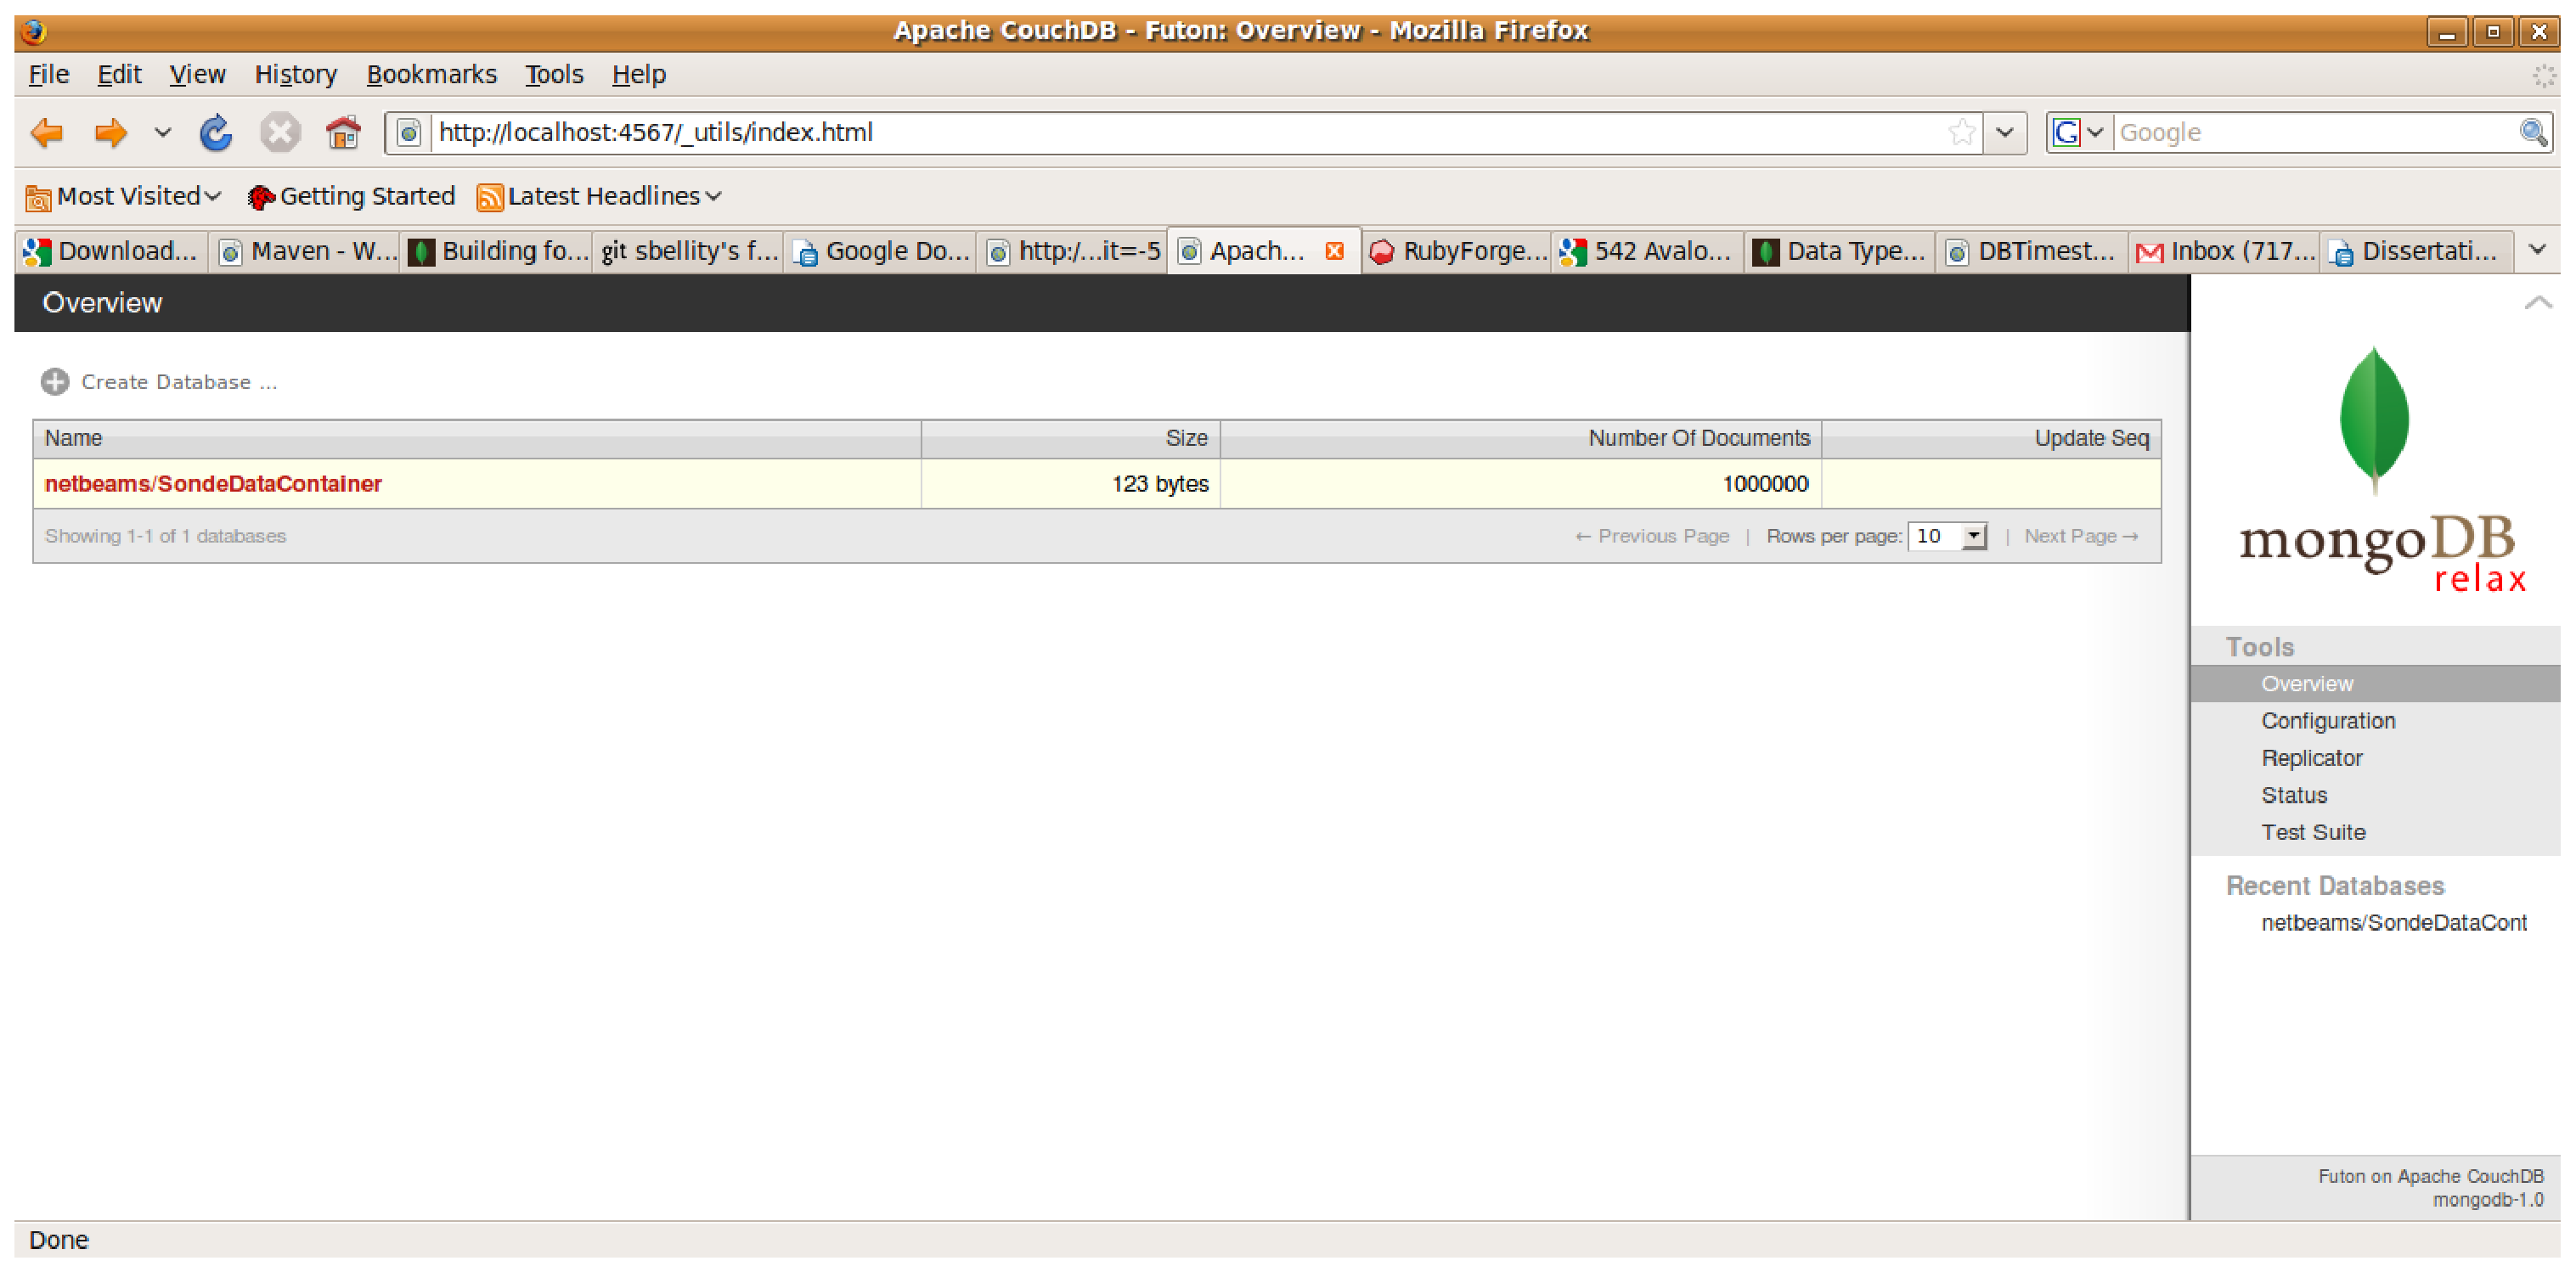
\includegraphics[scale=0.3]{../diagrams/view-collections-instance-browser-futondb}
  \caption{Viewing a partial list of data using the Futon for CouchDB/MongoDB}
  \label{fig:view-collections-instance-browser-futondb}
\end{figure}

The collection is composed by instances of documents of representing the YSI
Sonde type, being indexed by a document ID and the values being the keys
defined in the previous chapter, as shown in figure
\ref{fig:view-collected-data-list-browser-futondb}.

\begin{figure}[h]
  \centering
  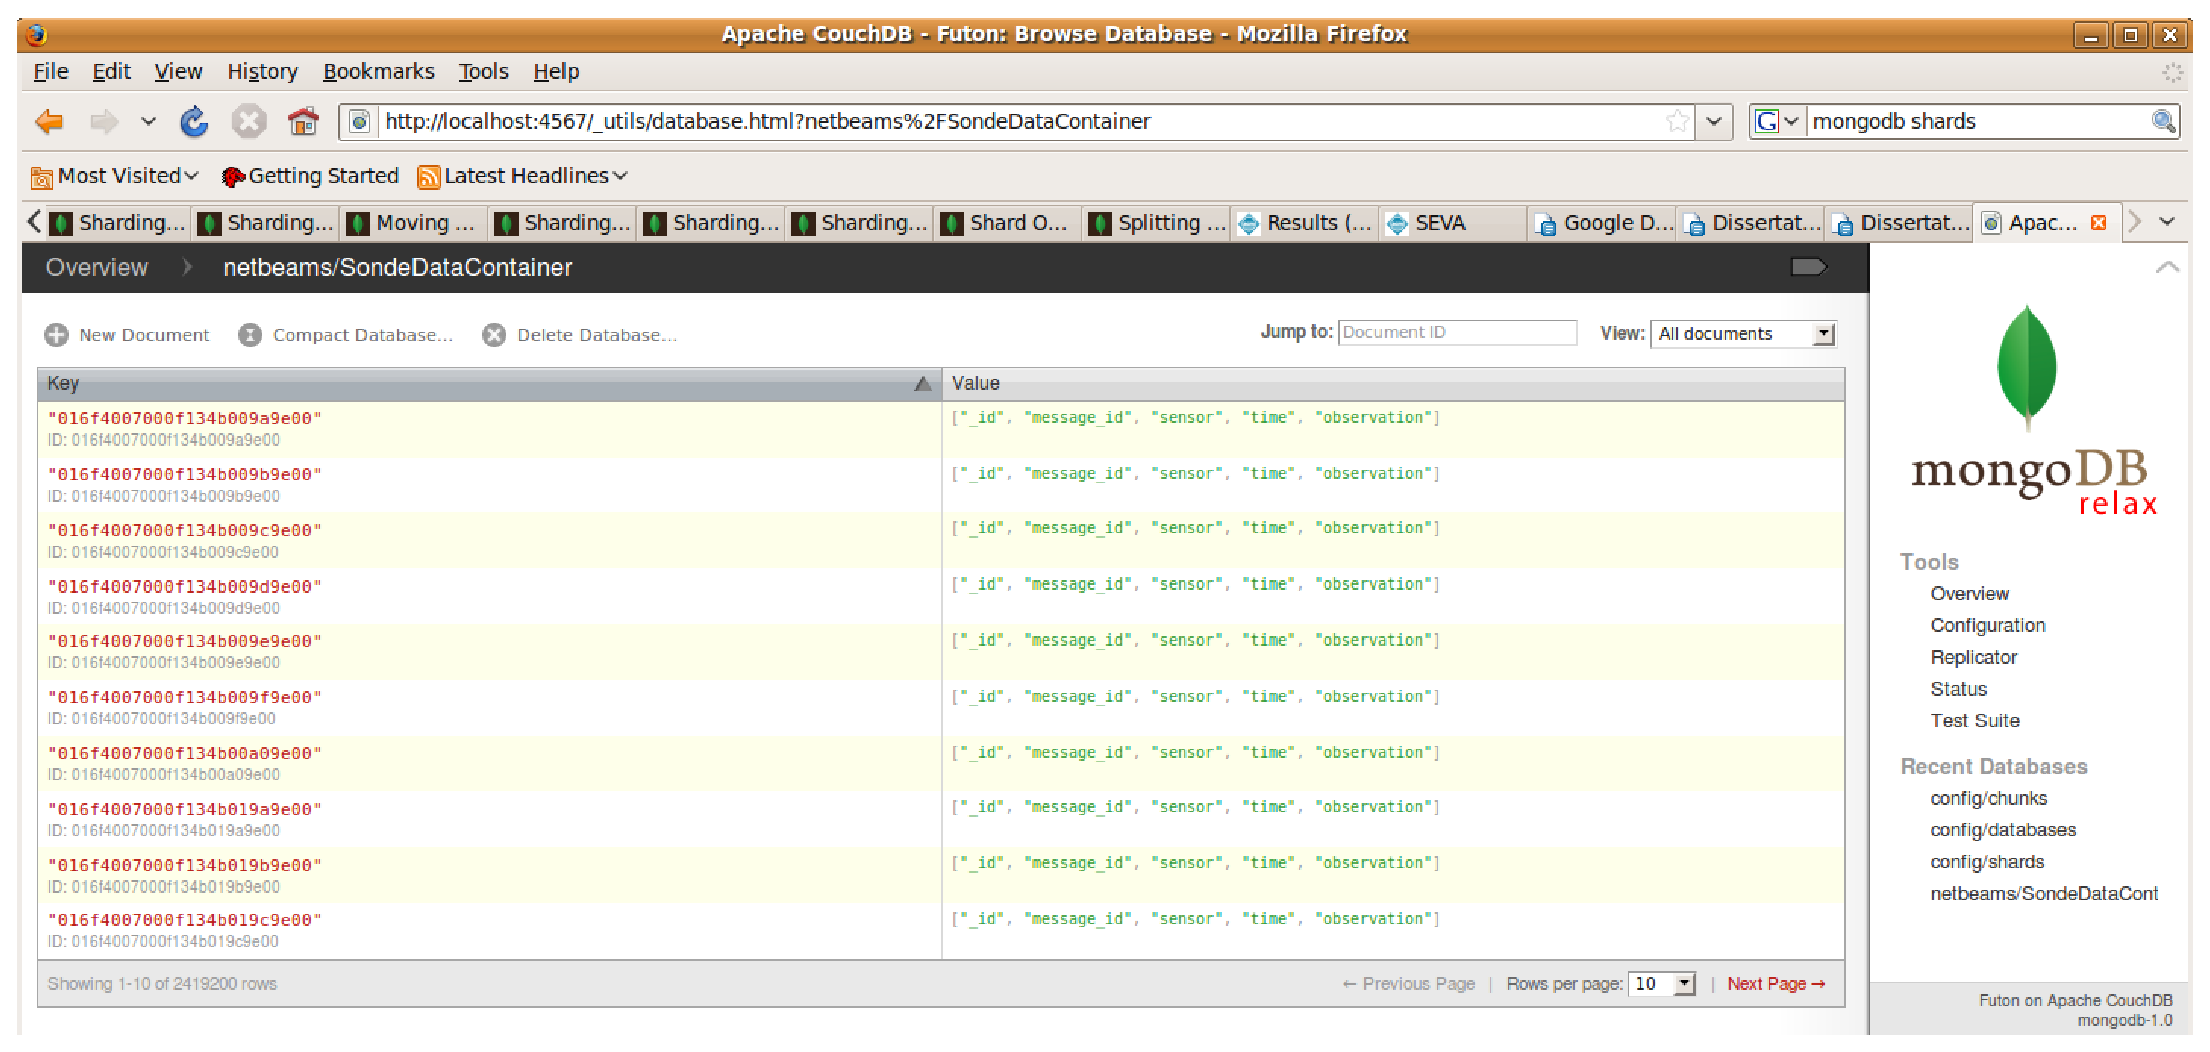
\includegraphics[scale=0.3]{../diagrams/view-collected-data-list-browser-futondb}
  \caption{Viewing a partial list of data using the Futon for CouchDB/MongoDB}
  \label{fig:view-collected-data-list-browser-futondb}
\end{figure}

By clicking in one of the items, one can view the instance of the document, as
it is shown in figure \ref{fig:view-collections-instance-browser-futondb}.

\begin{figure}[h]
  \centering
  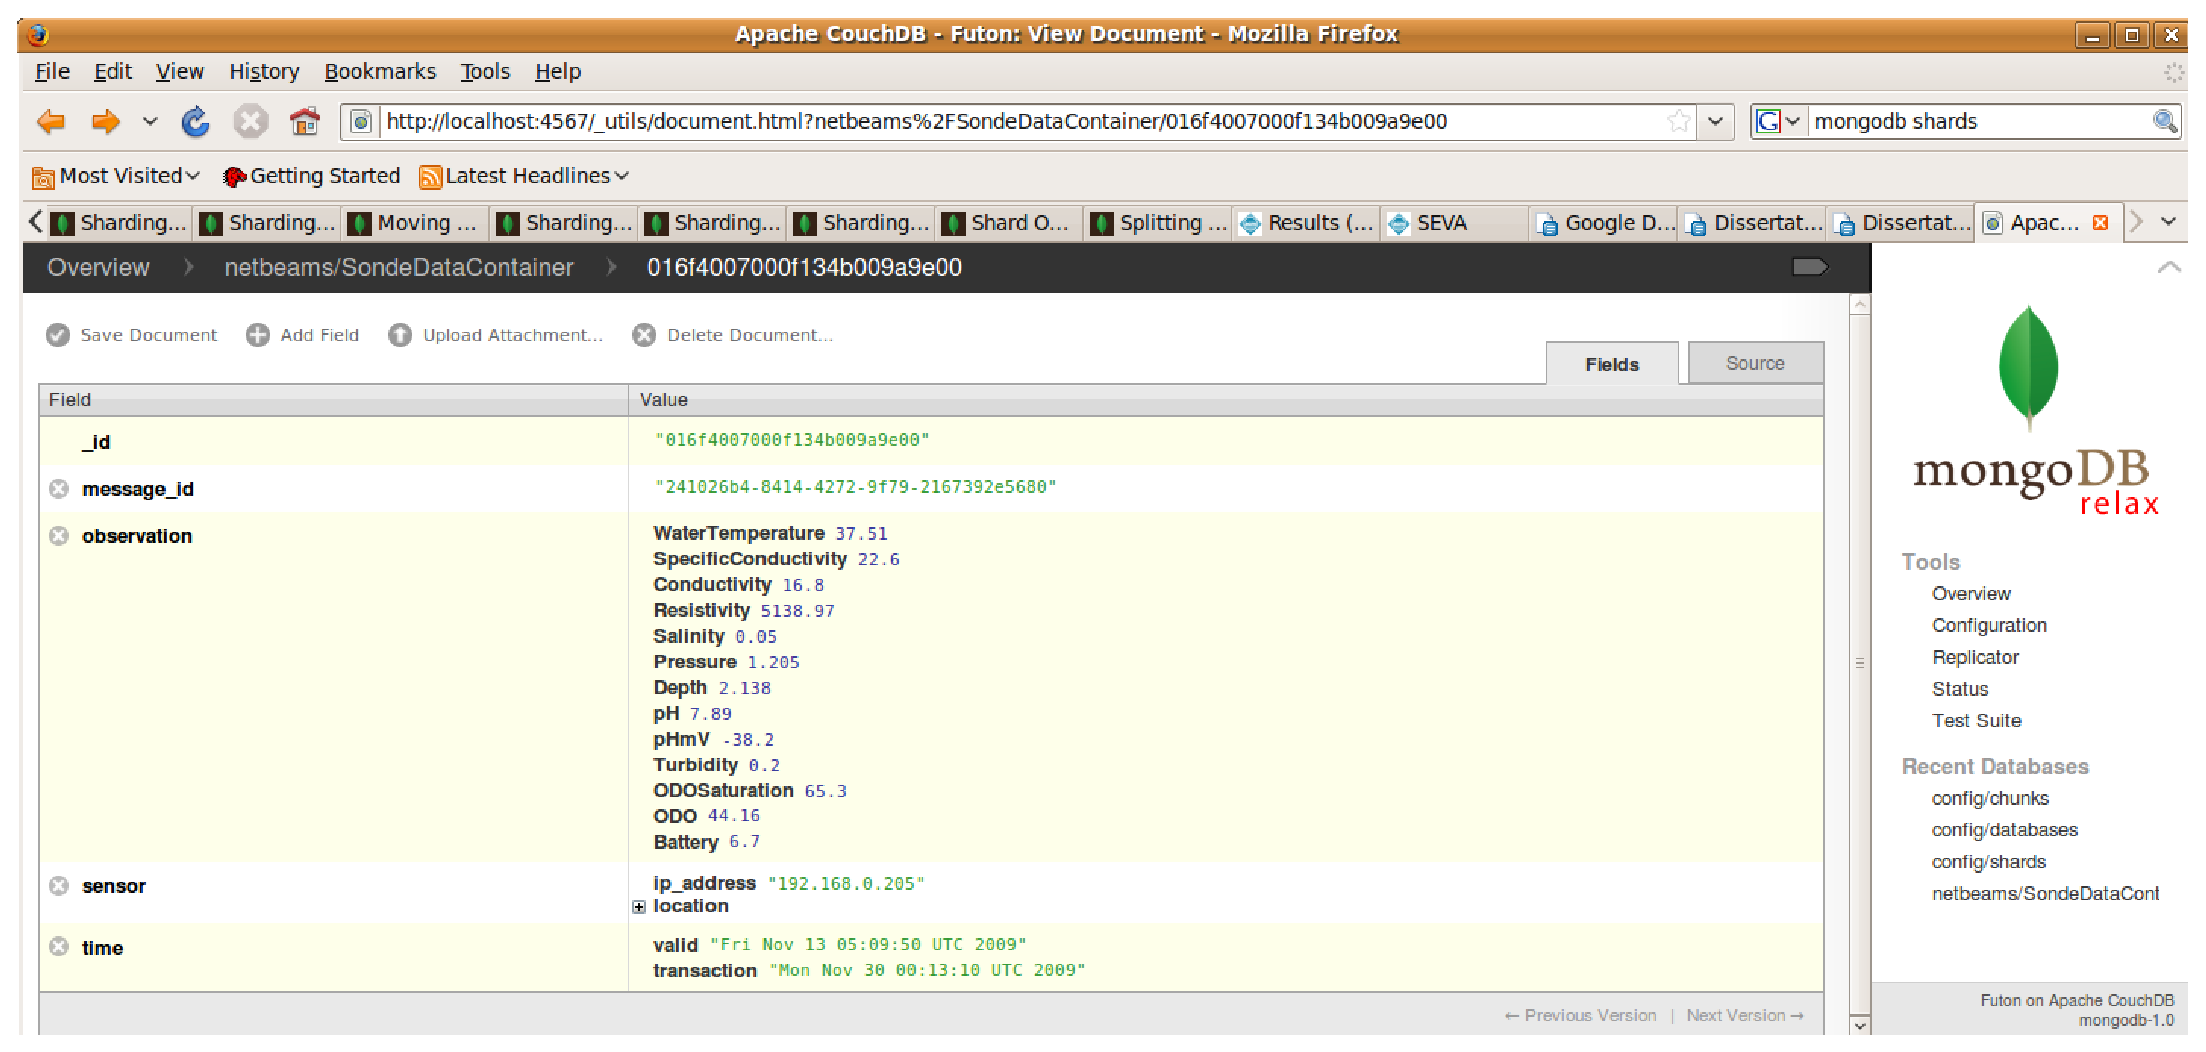
\includegraphics[scale=0.3]{../diagrams/view-collected-data-instance-browser-futondb}
  \caption{Viewing an instance of collected data using the Futon for
  CouchDB/MongoDB}
  \label{fig:view-collected-data-instance-browser-futondb}
\end{figure}

\section{Exporting Data to Spreadsheets}

mongoDB has an export facility shell called mongoexport. It can export the data
in JSON format or CSV. One may also write its own export tool in any of the
languages such as Java, PHP, Python, Perl, Ruby, among others. A list of the
existing drivers in different languages is provided
athttp://www.mongodb.org/display/DOCS/Drivers. The following command can be
executed to have the exported version of the data in CSV (read the help output
of the command for details).

An example to export the data in CSV format can be seen in listing
\ref{cmd:mongoexport}, and an example containing 1 million objects can be
downloaded at
http://netbeams.googlecode.com/files/experiment-1000000-data-exported-20090913-053538.csv.tar.gz.

\lstset{label=cmd:mongoexport,caption=Command to export data in CSV format}
\begin{lstlisting}
mongoexport -d netbeams -c SondeDataContainer --dbpath ./data/ --csv -f "_id,sensor_ip_address,transaction_time,fact_time,
data.temperature,data.sp_condition,data.condition,data.resistence,data.salinitude,data.pressure,data.depth,data.ph,data.pH_mv,data.odo_sat,
data.odo_condition,data.turbidity,data.battery" -o sonde-data-exported.csv
\end{lstlisting}

\section{Exporting Data to OPeNDAP Format}

By using any programming language driver, one can export data in the OPeNDAP
format.
% main.tex, to be used with thesis.tex
% This contains the main work of your thesis.

%\bibliography{thesis}  % uses the references stored in Chapter1Radar.bib

\chapter{Experimental Results: Correct Behavior and Performance}

As discussed in the previous chapter, the implementation of a data persistence
layer for NetBEAMS followed the requirements defined in Chapter 4 in regards
to the classification of the SF-BEAMS sensor network and the software
infrastructure provided by the Data Sensor Platform. The implementation was
developed using the infrastructure provided by the online version-control
system repository from NetBEAMS, whose documentation is detailed in Section
\ref{sec:dsp-data-persistence-implementation}.

This chapter details the experiment setup designed to evaluate the proposed
implementation, showing the measurement results collected from the simulation
log and based on the user experience while reusing the collected data. The
pertinent discussion of this work is divided up into different sections, each
of them analyzing different aspects related to data persistence for NetBEAMS.
Section \ref{sec:exp-setup} introduces the experiments setup and methods used
for the evaluation such as the artifacts used, the definition of the workload
to be used during the evaluation of the planned scenarios of evaluation. Then,
Section \ref{sec:exp-measurements} shows the measurement results of the
experiment detailing the operations performed by each of the scenarios and
user experience, to finally proceed with the final analysis and discussions.

\section{Experiment Setup}
\label{sec:exp-setup}

The experiment was designed to support different scenarios of regular use of
the mongoDB system infrastructure, simulating the activities of data collection
from the SF-BEAMS network using the NetBEAMS infrastructure. First, the setup
for the data collection of randomly generated data was implemented, which
directly uses already existing NetBEAMS classes. The CRUD scenarios were
implemented in different programming languages, from the data insertion
scenario using the Java Programming Language, to the remaining operations using
the Javascript Scripting language \cite{javascript} and the Python Programming
Language \cite{python}. Similarly, an open-source web application, developed
in the Ruby Programming language \cite{ruby}, was also used. The experiment
scripts were written using Shell Bash Script Language \cite{bashshell} and is
responsible for orchestrating the execution of one single experimental ``run''.

\subsection{Experiments Artifacts}

Different artifacts were created to perform the different experiments regarding
the CRUD operations. The ``Create'' operation' was developed in Java, isolating
the services provided by the class DSPMongoCRUDService (Listing
\ref{file:dsp-mongo-service}, page \pageref{file:dsp-mongo-service}). It is
responsible for the connection handling with mongoDB, as well as the insertion
operation from NetBEAMS. As described \cite{netbeams-dsp-architecture}, the
current version of NetBEAMS supports the data collection for the YSI Sonde
device \cite{YSI-Sonde}, among others used for demo purposes.

In order to exercise mongoDB with the same data collected from NetBEAMS, the
existing Java class TestSondeData (Listing
\ref{file:random-ysi-data-generator}, page
\pageref{file:random-ysi-data-generator}), was refactored to provide a random
instance generator for the YSI Data handler implemented in the Java class
SondeDataType (Listing \ref{file:main-ysi-data-handler} on page
\pageref{file:main-ysi-data-handler}). When the Insert function is executed,
the created instances are transferred from the JVM to the mongoDB, and stored
in the collection ``SondeDataContainer''. Specific details about the execution
of mongoDB are depicted in Section \ref{sec:mongodb-deployment}. Finally, the
implementation of the experiment in the Java class
DSPMessageToMongoDBExperiment (Listing
\ref{file:experiment-dsp-java-executor}, page
\pageref{file:experiment-dsp-java-executor}) was responsible for managing the
creation and insertion of any workload composed by instances of the class
SondeDataType in a bulk manner.

Similarly, the support for the Retrieve, Update and Delete operations against
the inserted workload were implemented using Javascript, as shown in Listing
\ref{file:experiment-scenarios} on page \pageref{file:experiment-scenarios},
respectively by the function calls ``find'', ``update'' and ``remove'' over
the collection ``SondeDataContainer''. Similarly, in order to implement a
customizable export system that converts from mongoDB into the format OpenDAP,
a simpler prototype script was developed in Python, as shown in Listing
\ref{file:experiment-export-python} on page
\pageref{file:experiment-export-python}. As a result of the execution of this
script, the exported artifact has the same format as described in Listing
\ref{file:rtc-ysi-opendap}, page \pageref{file:rtc-ysi-opendap}.

On the other hand, the execution of the main experiment shell script requires
the user to provide the size of the workload, as shown in listing
\ref{cmd:run-persistence-experiment}.

\subsection{Used Workload}
\label{sec:workload}

The workload selected for the experiments reflects the current use of the
collected data at the SF-BEAMS infrastructure. In this way, the experiment
runs for 5 different times to investigate different scenarios. This number is
related to the total number of sensor devices reported to be in operation, as
discussed in Section \ref{sec:sfbeams}. The volume of the workload prepared
after the experiment setup is as follows:

\begin{itemize}
  \item \textbf{First Round}: 483,840 documents, worth of production of the 
  YSI Sonde device during one year, at the rate of 1 observation per minute;
  \item \textbf{Next Rounds}: 483,840 * 4, or 2,419,200 documents, representing
  5 different YSI devices similar to the first round.
\end{itemize}

\subsection{System Environment}

Two different system environments were prepared: one for the External Storage
environment, or Single Server; and another for the Data-Centric Storage, or
Distributed Server. Since the single server is a regular centralized database
system, mongoDB just requires the execution of the database process ``mongod'',
which is started by specifying the directory where the inserted data will be
managed. The distributed server setup requires a different list of processes
(see Section \ref{sec:mongodb-user-experience}): one ``mongod'' process for
each mongoDB shard running on the different mongoDB cluster, one ``mongod''
process to manage the cluster metadata, and one ``mongos'' process, which is
the main one responsible to orchestrate the cluster. The single system
environment is symmetric to the External Storage used to persist the collected
data, while the clustered one simulates the Data-Centric Storage one.

The simulation of both the single and distributed system used both a Mac OS 10
Snow Leopard 64bit, with a total of 8GB of physical memory. However, in order
to simulate different shards in different machines, the use of a VirtualBox
\cite{virtualization} provided the use of guest operating systems to run and
act as the mongoDB shards. In this way, two different versions of the Ubuntu
Linux were used: one 8.04 32bits and another 9.04 64bits. The configuration
used for the single server only uses the process ``mongod'' to be started,
while the clustered setup must be enabled in the database, as in Section
\ref{sec:experiments-setup-single-distributed}.

\subsection{Planned Scenarios}
\label{sec:exp-scenarios}

In order to verify the feasibility of the solution proposed, all CRUD
operations were exercised through the implementation of the practical
scenarios based on the use cases described in Section \ref{sec:use-cases}. In
brief, the use cases were chosen to run with random values such as follows:

\begin{itemize}
  \item (R0) Insert a volume of collected data from sensors using NetBEAMS
  service compatible with 1 year of observations;
  \item (R1) Find all documents whose observations were collected between two
  different dates, say the days between December 8 and 15 of 2009;
  \item (R2) Find all documents whose observations were collected from a given
  known sensor device such as one whose IP address is equals to "192.168.0.102";
  \item (R3) Find all documents whose observations contained specific values
  read from the environment, say Salinity equals to 0.01 and the water temperature
  equals to 46.47;
  \item (U1) Update all the documents whose observations were collected during
  the day of December 2nd, 2009, by adding a tag = ``oil spill'';
  \item (D1) Remove all the documents whose observations were collected on
  December 7th, 2009.
  \item (R4) Export the produced data of the week to CSV files, using the same
  tabular format sequence used in the files distributed by SF-BEAMS using the 
  the OPeNDAP format, as in Listing \ref{file:rtc-ysi-opendap} on page
  \pageref{file:rtc-ysi-opendap}.
\end{itemize}

\section{Measurement Results}
\label{sec:exp-measurements}

As described in the previous section, the design of the experiments were based
on the specifications of a data persistence for NetBEAMS, using the mongoDB
database system. After setting up the experiment environment, the execution of
the workload was performed against the mongoDB database using its mechanisms
used to manipulate the data generated. It uses the programming language
abstraction to provide access and modifiy the data collected from the NetBEAMS
component. For this reason, this section details these mechanisms used to
implement each of the scenarios defined in the previous section, associating
numerical response time collected from the logs.

\subsection{Insert Operation}

The first set of measurements collected were the ones regarding the use case
R1, shown in Listing \ref{file:dsp-mongo-service} page
\pageref{file:dsp-mongo-service}, defined as the insertion of instances of the
collected data from the sensor devices using Java. The document follows the
specification of the keys designed in Section
\ref{sec:dsp-persistence-data-model}. The construction of the keys and
respective values were done using a Hash-like object ``BasicDBObject'' such as
the ones shown in the method ``buildKeySegment''. Similarly, the creation of
database indexes was performed using the same approach, as shown in the Java
method ``setupMetadataIndexes''. Then, the insertion of the documents was
performed on the service method call ``insertPersistentUnitMessageContents'',
which delimits the bulk creation using the transaction management mechanism
over the collection. In this way, different insert times were collected from
the logs of the different experiments as summarized on Table 7.1.

\begin{table}[!h]
    \begin{center}
        \begin{tabular}{|p{100pt}|p{100pt}|p{100pt}|}\hline
           x & \textbf{Linux VirtualBox Server} & \textbf{Mac OS Host Server}\\\hline 
           \textbf{Single Server} & ~25K docs/sec & ~51K/sec \\\hline
           \textbf{Clustered Server} & ~17K docs/sec & ~39K/sec \\\hline
        \end{tabular}
        \caption{Insertion averages on Virtual and Host in Single or Clustered
        mongoDB Server}
    \end{center}
    \label{tab:experiment-insert-avarage}
\end{table}

After executing the experiment, the claimed disk space for the representation
of the randomly generated data was separated into two different sizes: one
related to the amount of data produced by one YSI device, and another produced
by five different YSI devices, as summarized on Table 7.2.

\begin{table}[!h]
    \begin{center}
        \begin{tabular}{|p{100pt}|p{100pt}|p{100pt}|}\hline
        x & \textbf{1 YSI} & \textbf{5 YSIs}\\\hline
        \textbf{Indexed Keys} & 278.33 MB & 1.35 GB \\\hline
        \end{tabular}
        \caption{Amount of disk storage used}
    \end{center}
    \label{tab:experiment-insert-diskspace}
\end{table}

\subsection{Retrieve, Update and Delete Operations}

The simulation of the use case scenarios for the implementation used the mongoDB
shell client, which uses Javascript, for most of the operations for
``retrieve'', ``update'' and ``delete'' shown in Listing
\ref{file:experiment-scenarios}. The implementation of the use case to export
the collected data to OPeDAP format used Python, depicted on Listing
\ref{file:experiment-export-python}. The access pattern to use the collected
data is ``db.collection\underline{ }name.operation", where
``collection\underline{ }name'' is the name of the collection used for the
collected data, and in this case, the name of the DSP component that
represents the collected data. Therefore, mongoDB uses dynamic object binding
for the collection object, and executes the CRUD operations as method calls
with a list of the needed parameters. Table 7.3 relates method calls used to
implement each of the use cases defined, as implemented in Listing
\ref{file:experiment-scenarios}.

\begin{table}[!h]
    \begin{center}
        \begin{tabular}{|c|c|c|c|}\hline
        \textbf{Scenario Type} & \textbf{Language} & \textbf{Method Call} & \textbf{Use Case}\\\hline 
        \textbf{Insert} & Java & db.SondeDataContainer.insert() & R0\\\hline
        \textbf{Retrive} & Javascript & db.SondeDataContainer.find() & R1, R2, R3\\\hline 
        \textbf{Update} & Javascript & db.SondeDataContainer.update() & U1\\\hline 
        \textbf{Delete} & Javascript & db.SondeDataContainer.remove() & D1\\\hline
        \textbf{Export} & Python & db.SondeDataContainer.find() & R4\\\hline
        \end{tabular}
        \caption{mongoDB method calls used for the use cases}
    \end{center}
    \label{tab:experiment-scenarios-mongo-methods}
\end{table}

The execution time for each of the use cases were collected using the logs
collected during the execution of the experiment script manager. The retrieval
operations ran in average for 300ms, while the updates took more than 10
seconds when it involved larger data sets with more than 300,000 documents.
Similarly, the delete operation took less than 13 seconds to perform.

\subsection{User Experience}
\label{sec:experiments-user-experimence}

In general, the user experience of mongoDB is related to the methods used to
access and modify the state of the database using a different approach when
compared to traditional Relational databases. Since most of the methods to
create, access and modify the database were performed using the programming
language abstraction of objects and method calls, the transition from the use
of a relational data model is very easy. The creation of data was the first
contact with mongoDB in terms of data creation in Java. Later, different
methods of data access were used after the randomly generated data was
inserted into mongoDB: using the shell commands mongo and ``mongoexport'',
command-line execution developed in Python, through the REST Web Services API,
and using a web application, written in the Ruby Programming Language
\cite{ruby}, providing the view over the collected data using a web browser.
More details about the execution of these commands during the experiments are
shown in Section \ref{sec:mongodb-user-experience}.

The primary method used to access the mongoDB database is using the shell
command. Once the user requests access to the database, he or she can issue an
operation over the collection of documents using regular the abstraction
programming language, as the shown in Listing \ref{file:experiment-scenarios}
on page \pageref{file:experiment-scenarios}. The CRUD operations are available
to the user and can be used at any time to any database collection.
Aggregation operations such as to count the returned result set is also
provided via programming languages abstraction.

In order to export the collected data to other data formats, the  command
``mongoexport'' and the developed export script written in Python were used.
The ``mongoexport'', exports the collected data from the database using the
native support to comma-delimited values. As shown in Listing
\ref{file:mongodb-export-command}, page \pageref{file:mongodb-export-command},
the actual execution describe how mongo is querying the data from the
database. As a result, the total number of documents exported is shown in on
line 8. In addition to the regular command that exports the entire database,
the user can provide a query string during the execution of the command in
order to filter the dataset returned and, consequently, the number of
documents exported. Similar to the use of the default export capabilities of
mongoDB, a script written in Python to export data from mongoDB was written as
shown in Listing \ref{file:experiment-export-python}, page
\pageref{file:experiment-export-python}. It uses the package ``pymongo'' to
create a comma-delimited file with the same header and line format as shown in
Listing \ref{file:experiment-export-python-results}, page
\pageref{file:experiment-export-python-results}. The results can be compared
with the example the output of the HTTP Response body of Listing
\ref{file:rtc-ysi-opendap} on page \pageref{file:rtc-ysi-opendap}, requested
directly to the OPeNDAP server of RTC. Therefore, the experiment is capable of
reproducing the targeted OPeNDAP format used by the RTC server.

While the access to the database using the shell command gives full access to 
the CRUD operations, the access to the data was also performed using the REST
Web Services API, as shown in Listing \ref{cmd:mongo-rest-request} on page
\pageref{cmd:mongo-rest-request}. As one can see, the IP address and the
default port number of the mongoDB REST middleware are provided. Then, the
REST operation uses the name of the database and the collection to correlate
with the ones in the database system. Thus, querying the collections from
mongoDB can be performed using the HTTP Request Parameter variables, by adding
the prefix ``filter\underline{ }'' before the name of the key of the document.
The given example shows the query performed in the collected data for the key
``observation.Conductivity'' with the value ``104.5''. Similarly, the HTTP
Request variable ``limit'' is used to reduce the number of documents returned
by the query. The HTTP Response from mongoDB returns the result using the JSON
format, similar to the ones printed in the command-shell.

Finally, the access of the collected data was performed using Futon4Mongo,
an open-source web-based application written in Ruby that provides access to the
mongoDB database collections and documents. The screenshots of the session used
to browse through the collection of collected data is shown in Figure
\ref{fig:view-collections-instance-browser-futondb}.

\section{Discussion}

The implementation of the data persistence for NetBEAMS follows the
specifications explained in Chapter 4. The purpose of the sensor network for
NetBEAMS is to support data archival from any collected data, and for this
reason, mongoDB was selected after an empirical analysis described in Chapter
5. The requirements described in Chapter 4 were expressed as examples of use
cases in Section \ref{sec:exp-scenarios}. This chapter discusses the
experiments from different angles: analysis of the taxonomies, the
infrastructure, the use cases evaluation and applicability in other projects.

\subsection{Taxonomic Evaluation}

After selecting mongoDB as the best candidate for the persistence
infrastructure for NetBEAMS, the development of the persistence layer met the
requirements of archiving data for different types of sensor devices from the
DSP Platform such as the YSI Data Handler. As it is shown in Section
\ref{sec:exp-measurements}, the collected data is archived in files using the
BSON format \cite{bson}, a binary representation used to store instances of
the document described in Listing \ref{file:mongodb-ysi-data-format} on page
\pageref{file:mongodb-ysi-data-format}. Along with the purpose of Data
Archival, the use of mongoDB also met the specification of External Storage,
since the data persisted in the file system, as well as Data-Centric for
running mongoDB with different distributed mongo shards (cluster nodes).

SF-BEAMS uses Tabular Data model, a schema-less data model that represents the
collected data using comma-delimited files, without a database system to manage
those files, just the OPeNDAP middleware. In contrast, the data persistence
method proposed by this work suggests mongoDB as a schema-less database system
to manage the data collected using NetBEAMS. As described in Chapter 5, the
schema-less data model can provide better support to Data Provenance because
the data model allows the change of records without affecting the
others. In this way, the metadata used by the implementation clearly describes
the three fundamental questions regarding the collected data from sensor
devices, as described in Section \ref{sec:dsp-persistence-data-model}. The 
identity of the data is given by the key ``message\underline{ }id'', in a way
that it uniquely identifies the data produced. Thus, the message can be tracked
back to the sensor that produced the data for different purposes such as
tracking the data producer. Then, time dimensions were used in order to
track two different aspects of the data collection: the valid time can be used
to correlate observations to the exact moment it occurred, while the
transaction time can be used to verify when the data was collected, and make
decisions such as deleting the instances of data collected in the previous two
days, etc. Similarly, the use of the key ``sensor.location'' can give the exact
location of the data, since researchers can be interested in finding data
based on a specific location. The most important aspect of the schema-less data
model is that the observed data is added to the key ``observation'', as any
sensor device carries its set of attributes of key-value pairs. A good example
of the applicability of the schema-less model is the scalability regarding
changes to the data structure. For example, if an existing sensor device is
flushed with a new version of the firmware\footnote{Primary machine
instructions that run in the hardware}, changing the format of data types or
adding new values, the following instances of collected data may very
from the previous one by simply adding the new additions of data. For this
reason, the DSP Data Persistence gives administrators the ability to choose
which fields to persist by declaring it using a bootstrap message for the
component, as shown in the parameter ``YSI\underline{ }DESIRED\underline{
}PROPERTIES'' of Listing \ref{file:dsp-data-persistence-bootstrap.xml}, page
\pageref{file:dsp-data-persistence-bootstrap.xml}.

In order to access the collected data, the implementation used different APIs
provided by the mongoDB community. The Centralized Query Mechanism was
satisfied by the use of those APIs, which also fulfills the requirements
defined by NetBEAMS. For example, the accesses of the database using Python or
Java were based on the needs and the use of the languages for different
purposes. In this way, the implementation of the persistence model captures
the instances of any known data collected from NetBEAMS and saves it using the
document pattern as shown in Listing \ref{file:mongodb-ysi-data-format} on page
\pageref{file:mongodb-ysi-data-format}. Any programming language used was
capable of accessing the same collected data by their own. 

In the end, the implementation of the data persistence for NetBEAMS was
developed in both Centralized and Distributed Systems. The use of regular single
server execution provided enough computational power for a compatible volume of
data when compared to the one produced from the SF-BEAMS sensor network. The
implementation suggested by this work fulfills the needs of a persistence system
for a Small volume of data being created at the same time in a Single Server.
Furthermore, mongoDB also provided support for a Distributed System, when the
use of database shards, in forms of different mongoDB nodes, was used as a 
clustered environment.

\subsection{Infrastructure Evaluation}

Overall, the implementation of the DSP Data Persistence component meets the
specification of the use cases defined in Section \ref{sec:exp-scenarios}.
From the perspective of disk-space utilization for the compatible volume of
data for five YSI devices is that it requires a small amount of disk space.
According to the mongoDB documentation \cite{mongodb}, the claimed amount of
disk space is related to how mongoDB uses a binary representation of the JSON
documents, which are composed only of strings, together with the definition of
the indexes. The size of the keys defined for the YSI Sonde data suggests
additional disk space was used for the storage.

The performance to insert data into the database system using the Java driver
is documented by mongoDB as the fastest approach, providing persistence for
thousands of documents per second. This capacity is more than adequate for
NetBEAMS, which can use the Single System environment. Improvements over the
response time can be achieved through the implementation of a Data-Centric
approach on a Distributed Database environment, or clusters. In this approach,
the inserted data is stored in different servers based on a partition key.
Given that less data is concentrated in each partition, the centralized query
mechanism used is faster, and consequently improves the performance as
described in the Data Location taxonomy in Chapter 3. In this way, the
infrastructural performance during the inserts suggests that persisting data
collected from the NetBEAMS sensors using a clustered environment is an option
when the single server capacity is reached.

Different problems and limitations were faced during the execution of
mongoDB, which were related to the infrastructure used: the limitations
regarding disk storage in 32bit operating systems and very slow
performance when using virtualized servers. During the execution of the
experiments, mongoDB used memory accordingly, without taking control of the
operating system's resources. However, when mongoDB is used in a 32bit server
architecture, there are limitations on the disk space used to store
collections. After reaching 2GB of collected data during many different runs,
mongoDB crashed and did not allow the use of the collected data. For this
reason, the setup of a new VirtualBox using Ubuntu Linux 64bits as a guest to
a Mac OS X 64bits was prepared and used throughout the completion of these
experiments. On the other hand, the performance was drastically decreased 
using mongoDB in virtualized servers due to the fact of dynamic partition
chosen. The performance shell application ``iostat'' was used to verify the
behavior, and the use of mongoDB was switched to the host operating system.

\subsection{Use Cases Evaluation}

\cite{sn-programming-language} suggested that programming languages are easier
abstractions to researchers that use collected data from sensor devices
without a background in computer science or database systems. The authors have
suggested the implementation of a programming language for this group of
biologists, for instance. This suggestion has good intentions, but
limits the users with a single mechanism to access the collected data from
sensors. For this reason, this report proposes the use of key-value pair
databases, such as mongoDB, to provide transparent access the data through
the abstraction of any programming language that has a driver written for
mongoDB. During the user experience section, different programming languages
were used to access the collected data, a novel mechanism not yet reported in
the sensor networks community.

The development of the scenarios were clearly written in different ways, such
as the ones defined in Listing \ref{file:experiment-scenarios} on page
\pageref{file:experiment-scenarios}, which implements the use cases for data
Retrieval, Update and Deletion operations. The main advantage of this approach
is that users do not use the SQL language to extract data from the database,
but use method calls defined for each the abovementioned operations. For
example, based on the description of the collected data by keys and values
shown in Listing \ref{file:mongodb-ysi-data-format}, page
\pageref{file:mongodb-ysi-data-format}, different use cases can evaluate
documents in this structure. Usually researchers may search the collected data
by a given range of dates, for their regular activities of data analysis. The
scenario implemented by R1 in the above cited listing shows it clearly.
Similarly, the search for data in a given sensor device is expressed by the
search for the IP address for them on the use cased defined by R2. Finally,
the search for the raw data obtained by the sensor devices is used from the
key ``observation'', as shown by the R3 use case implementation.

Allowing for non-predictable events that might occur during the data
collection process of sensor devices, which will influence their values, the
support to annotations is a feature that can be used to describe the data.
mongoDB indirectly supports the use of annotation because of its method
of updating documents and adding new keys to any of them without requiring
design changes. Supposing an environmental event occurs, such as the recent oil
spill in the San Francisco bay in October 2009 \cite{sfbay-oilspill2009}, the
values of the collected data, and data analysis, was influenced by different
presence of different objects in the water. The implementation of the scenario
U1 provided the addition of a new key called ``tag'', with the annotation ``oil
spill''. This new key, after properly indexed, provides another option to
meaningfully search the collected data from the sensor devices. Old data then
can be deleted as expressed by the scenario D1, as a regular operation
supported by any database system.

Commonly during scientific research, data is shared. Researchers can choose
the use of spreadsheets to analyze collected data with simpler tools than
database systems or programming language. For this reason, OPeNDAP is used in
the community to share data using a comma-delimited format. In this way, the
implementation of the use cases for R4 was developed in two different ways.
First, the use of the export capabilities to a common-delimited values was
performed (Listing \ref{file:mongodb-export-command}, page
\pageref{file:mongodb-export-command}), taking proximally 3.3 minutes to export
one year's worth of data for 5 YSI devices without indexing. Second, the
implementation of a custom export utility using Python, as shown in Listing
\ref{file:experiment-export-python}, page
\pageref{file:experiment-export-python}, enabled the creation of the
comma-delimited files with the same format as the ones used by OPeNDAP. The
comparison can be done by analyzing the output of the OPeNDAP request from
SF-BEAMS on Listing \ref{file:rtc-ysi-opendap}, page
\pageref{file:rtc-ysi-opendap}, and the output provided from the script
written in Python, show in Listing \ref{file:experiment-export-python-results}
page \pageref{file:experiment-export-python-results}. Furthermore, considering
research teams with skills in Web Services, an easy ubiquitous integration
with mongoDB can be achieved by using the REST Web Services APIs provided by
mongoDB, still in alpha version. A practical application of this API was the
created Apache Futon4mongoDB web application, used to give user friendlier
access to the collected data as shown in Figure
\ref{fig:view-collections-instance-browser-futondb}, on page
\pageref{fig:view-collections-instance-browser-futondb}.
 
As discussed in Chapter 5, the differences between a traditional database
system, which uses the relational data model, and document-oriented database
systems were clearly noticed during the development of this work. As mentioned
in Section \ref{sec:experiments-user-experimence}, the user experience was
mostly related to the definition of the keys that describe the sensor device,
developed as discussed during the design of the solution in Chapter 6. 
Therefore, based on the use of a different type of data model in the scope of
data persistence for sensor networks, the taxonomies defined in Chapter 3
could be updated to the one shown in Figure
\ref{fig:taxonomy-data-model-modified}, including the Key-Value Pair Data
Model.

\begin{figure}[!h]
  \centering
  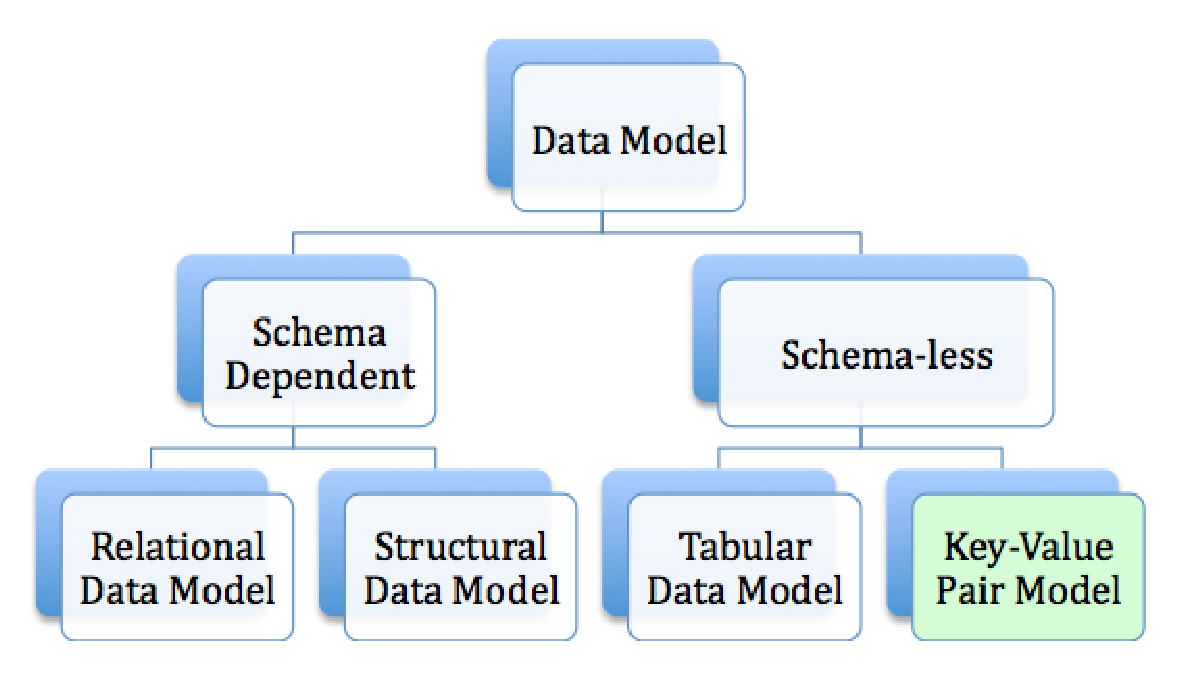
\includegraphics[scale=0.65]{../diagrams/taxonomy-data-model-modified}
  \caption{Updated Data Model Taxonomy, adding the KVP Data Model}
  \label{fig:taxonomy-data-model-modified}
\end{figure}

\subsection{Applicability and Recommendations}

This work can be used to evaluate data persistence in sensor networks in
different ways. The use of the data persistence taxonomies through this work
guided both the evaluation and implementation of the data model using mongoDB.
In order to use the guidelines proposed by this work, one may first determine
the properties of the sensor network in question. Considering that sensor
devices produce streams of non-described data, the use of key-value pairs data
model did not require changes throughout different application layers.

Focusing on the different layers of an application, consider the different
multi-tier application approaches where each layer implements a functionality
of the system such as the Model-View-Controler (MVC) \cite{sw-architectures}.
Usually, the use of traditional database systems and object-programming 
languages require ``data plumbing'' from the table relations from
the database system to the object instances. In order to implement all the
CRUD operations to a relational database without an ORM \cite{orm} offering,
the implementation of the data model potentially uses the Structured-Query
Language (SQL) for the problem of data plumbing, which results in a
tightly-coupled implementation. On the other hand, mongoDB eliminates the use
of an additional query language because it uses declarative approach on top of
the programming language drivers it support, decreasing the complexity of the
application.

Sensor networks with medium or large volumes of data are implemented nowadays
using clusters and parallel programming. Google's BigTable \cite{bigtable} uses
the principle of structured data in distributed tabular format, processing large
volumes of data using the MapReduce parallel approach \cite{map-reduce}. The
current version of mongoDB offers its first version of the MapReduce approach,
but it is still imature. However, it can be useful to process large amount of
data collected from sensor devices, or process historical data for any type of
analysis.

\subsection{Difficulties Experienced}
\label{sec:experiments-difficulties}

Particularly speaking about the learning curve, different situations
contributed to the success of the first experiments. The first problem to be
solved was the selection of the data model to be used during the technology
selection. Since relational database systems are the ``traditional'' way to
provide data persistence, the investigations started by creating a relational
model described in Chapter 5. Then, the technique using KVP data models in
relational databases were attempted without success. Only after reviewing the
technical article \cite{db-is-rdbs-dommed}, suggested the advisor of this 
work, the search for a database system that uses the KVP data model was
considered, and finally successfully implemented.

Since the technology is new, it brought new challenges regarding the usability
and user experience. The technology is relatively new and still under development,
many different bugs were be reproduced at random during the execution of
the experiments, and therefore, reports were sent to the open-source community
through various communication channels. To address this, the fastest way to
solve an issue was through the mongoDB's IRC channel located at the Freenode
server (www.freenode.org, channel mongodb). Second, the users group, located at
http://groups.google.com/group/mongodb-user also helped troubleshooting
problems.

Physical memory is limited and, for this reason, it may not be enough to run
the experiments for total workloads. In this case, the Java Virtual Memory was
totally consumed by one of the revisions of the experiments setup. Therefore, 
it was learned that large amount of data loads require different techniques to
manage data in memory accordingly, such as creating different object pools as
temporary caches for objects whose internal state are similar to others in the
JVM. Also, operations that involve writing in disk, such as during the bulk
``Create'' operations, may lead to different database performance. First, the
experiment seemed to stop inserting objects in one shard while it ran for over
2 minutes without inserting any documents. The reason was that the partition
was ``/home'', completely full, leading to the problem. The mongos cluster
header did not realize that it was the time to switch to another shard.
Similarly, any global ``Retreave'' operation on a cluster blocks all the
shards. For this reason, dividing the write from the read load was necessary
in order to decouple these two operation.

Also related to the difficulties of this work, mongoDB is not yet stable, and
therefore, harder to implement. The main production version of mongoDB
is on version 1.2 at this time, while the shards support is still in alpha
version. For instance, different work-arounds were performed to have shards
experimented as described, but the execution was not successful.

To sum up, this chapter described the experimental results of the
implementation of a data persistence component for NetBEAMS, showing the
experiment results, the measurement results and finally the discussion about
the solution in general. The following chapter brings the conclusions and
future works for this report.

% main.tex, to be used with thesis.tex
% This contains the main work of your thesis.

%\bibliography{thesis}  % uses the references stored in Chapter1Radar.bib

\chapter{Conclusions}

This work presented a collection of taxonomies related to data persistence for
sensor networks using different approaches ranging from data models and server
infrastructure organization. The main result of this work was that persistence
for collected data from sensors are better maintained using schema-less data
models, since it provides offers an approach to deal with unanticipated data
types from the sensor devices.

As seen in the state of the art, different approaches can be done in order to
evaluate data persistence for nsensor networks. T

There are many important features covered in this work, including the
importance of the sensor networks rely in how users have access to the
collected data. In order to provide access to the collected data, one must
first assess the different types of infrastructural characteristics of the
studied sensor network. In general, the selection of a technology that
provides such persistence capabilities can be part of a process of analysis of
taxonomies proposed by this work. However, this work proposes a data model not
yet used in the sensor network community and, thus, represents an important
contribution for the area.

Taking into account the software architecture provided by NetBEAMS, as well as
the requirements for data collection from the RTC research group, this work
shows a novice way to persist data collected from sensor devices by using a
schema-less data model, whose query capabilities are based upon programming
languages, in contrast to the use of the Structured Query Language, SQL. The
experiment results showed that the implementation of a persistence layer with
mongoDB can be used to persist data at its maximum rate of one sample per
minute. However, the evaluation of mongoDB was not used to implement a
Data-Centric Storage approach, which can decreases the amount of time to search
data since the process uses parallel search.

All in all, the DSP Data Persistence component implemented for the NetBEAMS
solution to SF-BEAMS can be used in any network server. The solution for data
persistence is a novice way to save data into the database, provided by
mongoDB's ability to cope with the uncertainty of any properties collected from
any sensor specification. Furthermore, the solution also provides a good
support to the provenance-related data as the schema-less data model gives the
ability to .


\chapter{Future Works}

0. Todo list for this work
1. Database System Problems
2. Software Engineering Problems
3. Applications
 - plot graphs of collected, 

There are many different directions for future works. First, the
implementation of a Data-Centric Storage approach can help the system scale
horizontaly by using the mongoDB's database shards. In this way, this approach
can reduce the retrieval time by focusing on centralized selection of data over
a given database shard. Moreover, the overall search through the collected data
attributes can be drastically decreased by parallel search over the database
shards using the MapReduce \cite{map-reduce} tools. At this time of
development, the MapReduce API offered by mongoDB is on its alpha version, and
therefore, presenting lots of bugs. Figure
\ref{fig:future-works-data-centric-map-reduce} shows an architectural idea of
the deployment of a Data-Centric storage approach. When searching for specific
document attributes, the process is sent in parallel to each of the database
shards, and the result is collected by the cluster head. After calculating the
final result, mongoDB server returns the relevant result to the user.

\begin{figure}[h]
  \centering
  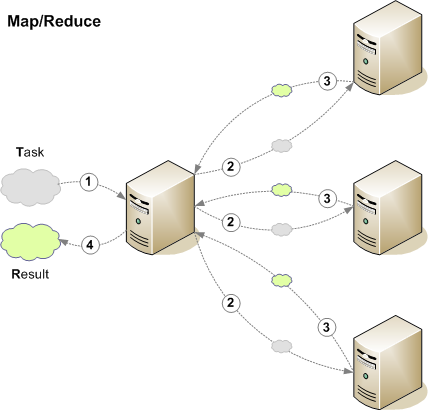
\includegraphics[scale=0.5]{../diagrams/future-works-data-centric-map-reduce}
  \caption{Data-Centric approach using MapReduce to search accross different
  database shards}
  \label{fig:future-works-data-centric-map-reduce}
\end{figure}

In addition to infrastructural, the use techniques for scheduling data
gathering from the SF-BEAMS sensor networks can be used to decrease the data
load into the system. While the period of times used by the RTC seems
to cover the basic requirements of data, the data storage may be
seen as overloaded with repeated data. Since environmental conditions
does not change drastically over time, the use of data scheduling and
data clustering approaches can be used. First, considering that SF-BEAMS
contains a cluster of sensors, the data load could be decreased by using
techniques such as clustering the data in the data sink before they are
persisted \cite{sn-time-series, sn-schedule-minimal-aggregation-time}. Since
the infrastructure of the SF-BEAMS sensor network is a one-hop start design,
the knowledge about the data can only be achieved in the data sink. In this
way, one suggestion is the implementation of a DSP Data Clustering component
that is responsible for the data clustering before they are inserted into the
database. Similarly, the use of schedulers on the sensors could also be used to
decrease the amount of data to be sent to the data sink, as seen at the survey
\cite{sn-scheduling-survey}. 

Finally, taking into account the use of the database system to complement
NetBEAMS execution, the design of event-based applications could add different
functionalities to the management capabilities of the sensor networks. For
instance, the YSI sonde collected data carries the information regarding the
battery life of the device, seen at the collected attribute 
``observation.Battery''. A new DSP Component responsible for observing these
attributes could define the threshold of the event of low-battery. With an
event-based application in mind, events regarding the SF-BEAMS network could be
better managed through NetBEAMS where scheduled sites visits would depend on
such events to happen and, thus, avoiding unecessary operational costs.

\appendix
\chapter{Appendix}

This section includes the source-code for the DSP Data Persistence. Each
section details one single main artifact used on the development of the
component. However, only the main ones will be added into this document, while
the remainder can be downloaded directly from the Subversion repository.

\section{The Data Sensor Platform (DSP)}
\label{sec:dsp-details}

The Data Sensor Platform, in short DSP Platform, is based on a micro-kernel
architecture developed on top of the Java modular framework called OSGi
\cite{osgi}. The platform represents the foundation of the execution of
NetBEAMS, since it is executed from an embedded hardware called Gumstix
\cite{gumstix} using a Linux operating system and on top of the Java Virtual
Machine (JVM). In order to transport data from sensors hosts to the network
sink, the use of a cellular connection is used to transport the collected data
from the senso devices using the HTTP Protocol, as described by
\citet{netbeams2009}. Figure \ref{fig:sf-netbeams-node} shows the
architecture of the inhanced node designed by the NetBEAMS research group.

\begin{figure}[h]
  \centering
  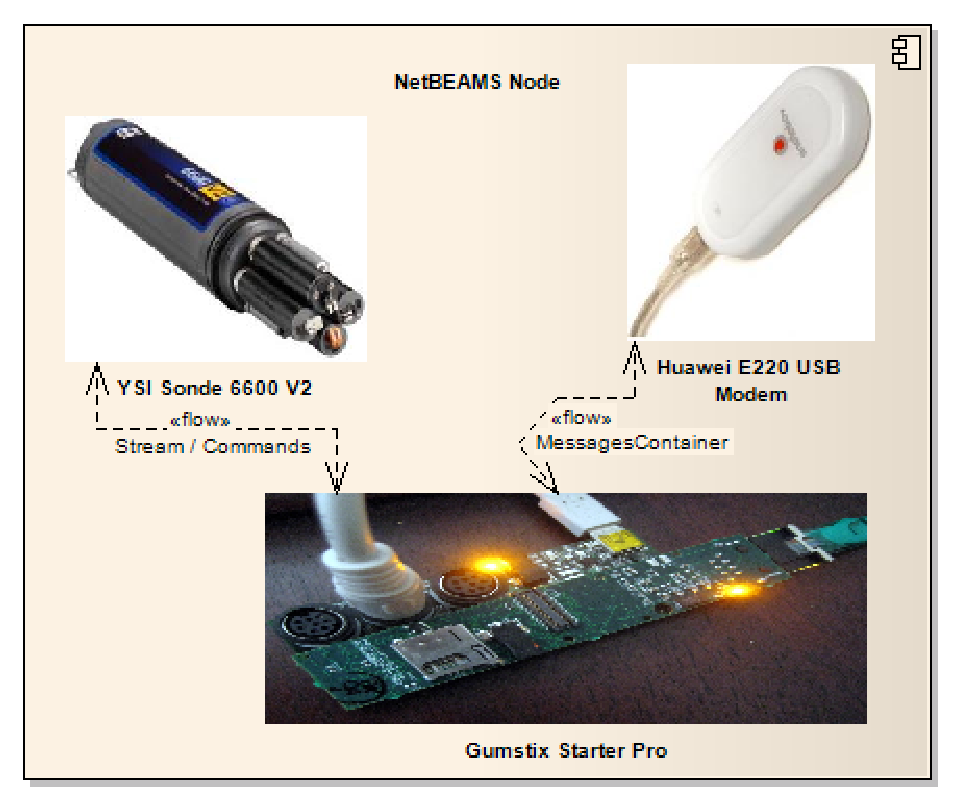
\includegraphics[scale=0.5]{../diagrams/DSP-Gateway-Node}
  \caption{The NetBEAMS Node enhancement with the Gumstix and the GSM Modem}
  \label{fig:sf-netbeams-node}
\end{figure}

The following list describes each of the devices in the NetBEAMS Node.

\begin{itemize}
  \item \textbf{YSI 6600EDS V2}: the YSI device is the regular sonde
  responsible for observing the environment. It is connected to the Gumstix
  embedded system, where the DSP is executed;
  \item \textbf{Gumstix console-vx}: it's a COTS ARM-based hardware that
  provides a computer-on-module environment for the development of small
  embedded systems. This is the main environment of data extraction and remote
  processing is accomplished. It runs a cross-compiled version of Linux Kernel
  2.6;
  \item \textbf{Huawei E220 USB Modem}: it is used to transfer the data from the
  Gumstix to the RTC Labs Data Center.
\end{itemize} 

The DSP runs inside of the embedded system Gumstix. The following sections
details its design and process for extracting data.

\subsection{The DSP System Design}

This section focus on the development of a Software Platform for the NetBEAMS
Gateway Embedded System, or on the system developed in the Gumstix device. As
shown in figure \ref{fig:netbeams-software-stack}, the NetBEAMS Gateway Node is
an embedded system that contains a set of layer found in any computer.
However, each of the resources described from the system were customized for
the NetBEAMS system. The main components of such system can be summarized as
follows:

\begin{itemize}
  \item \textbf{Operating System}: it uses a cross-compiled Gentoo Linux, which
  supports a wide variety of development tools, including the Java Virtual Machine
  (JVM), the underlying platform system;
  \item \textbf{Java Virtual Machine}: it uses the JamVM, a ~200 KB version of
  the Sun Microsystems Java Virtual Machine, version 2.0;
  \item \textbf{OSGi Framework}: it uses the Knopflerfish implementation of the
  OSGi 4.1 specification. More details in the following sections.
  \item \textbf{DSP Platform and other Bundles}: The plug-and-play DSP
  Components are based on the OSGi bundles capabilities, which can reuse services registered in the OSGi framework.
\end{itemize}

\begin{figure}[h]
  \centering
  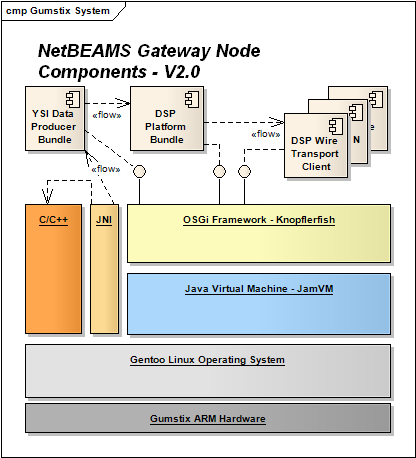
\includegraphics[scale=0.6]{../diagrams/NetBEAMS-Client-Node-Components}
  \caption{The NetBEAMS's Gumstix Software Stack}
  \label{fig:netbeams-software-stack}
\end{figure}

As depicted in figure \ref{fig:netbeams-software-stack}, the DSP Sonde Data
Producer component opens a serial connection with the device through the Java
Native Interface (JNI) driver and produces the data flow 1. The data stream
format at this stage is as described on table \ref{tab:ysi-data-stream}.
Later, by parsing and transforming the data to DSP internal representation, it
sends the data to the DSP Platform as depicted on flow 2. Finally, the DSP
Platform decides to send the data to the DSP Wire Transport Client, as shown
on flow 3, by following rules defined by the system administrator. At this
point, the data is ready to be transmitted to the server, which is covered on
the following sections.

\subsection{The DSP Platform Architecture}
\label{netbeams-architecture}

The architecture of the DSP, aligned with the OSGi capabilities, reuses the
Service-Oriented Architecture that can easily enable and disable plug-and-play
components. By following a publish-subscriber design-pattern \cite{gof}, the
service producer registers into the service broker while the consumer looks
for a given registered service in the Service Broker. For this reason, this
approach allows decoupled interoperability among modules as it is shown in
figure \ref{fig:publish-subscriber-pattern}.

\begin{figure}[h]
  \centering
  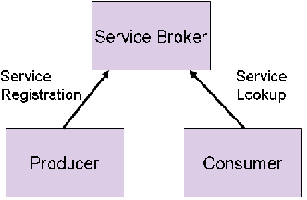
\includegraphics[scale=0.6]{../diagrams/publish-subscriber-pattern}
  \caption{The publish-subscriber design-pattern for services}
  \label{fig:publish-subscriber-pattern}
\end{figure}

The DSP infrastructure is based on a loosely-coupled architecture hosted in a
given host computer with an OSGi container, where the entire system is
composed by a set of plug-n-play OSGi modules. Each DSP component, as an
instance of an OSGi Module, can perform specialized tasks according to its
specification. In general, each DSP component can be categorized as follows:

\begin{itemize}
  \item \textbf{Data Producer (DP)}, whose main function is to produce data for
  the system;
  \item \textbf{Data Consumer (DC)}, whose main function is to consume the
  received data.
\end{itemize}

\begin{figure}[!b]
  \centering
  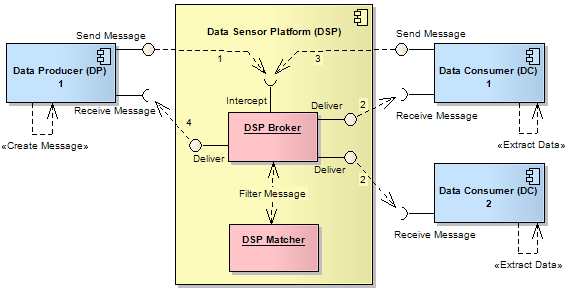
\includegraphics[scale=0.7]{../diagrams/DSP-Producers-Consumers-Components-Interactions}
  \caption{The basic architecture of a Data Sensor Platform (DSP)}
  \label{fig:DSP-Producers-Consumers-Components-Interactions}
\end{figure}

The Data Producers and Data Consumers exchange data through the DSP Message
Broker using a message unit called DSP Message. As it is depicted in figure
\ref{fig:DSP-Producers-Consumers-Components-Interactions}, a Data Producer
creates a set of one or more DSP Messages wrapped up in a DSP
MessagesContainer in order to be sent to the DSP Message Broker. When the
broker receives the set of DSP Messages, it requests a list of Data Consumers
to each of the DSP Messages based on rules managed by the DSP Matcher.
Whenever the broker acquires the list of Data Consumers, it delivers a copy of
the DSP Message to each of the Data Consumers in the receiving list. Upon the
DSP Message arrival, each Data Consumer can extract the actual data from the
DSPMessage. Finally, although the components can be distinguished between Data
Producers and Consumers, any of them are entitled to send and receive
administrative DSP Messages, which is covered in the following sections.

When the DSP Platform is installed into the OSGi framework, it follows the
OSGi specifications without any changes to remain it in the installed state.
In this way, it is important to note that the DSP Platform and its
plug-and-play components are directly mapped with the OSGi Framework as
follows:

\begin{itemize}
  \item \textbf{OSGi Bundle} = DSP Component Artifact in Jar format
  \begin{itemize}
    \item SondeDSPProducer.jar is the component developed for the YSI sonde
  \end{itemize}  
  \item \textbf{OSGi Activator} = DSP Component Activator
  \begin{itemize}
    \item Class specified in the MANIFEST.MF artifact (next sections)
  \end{itemize} 
  \item \textbf{OSGi Service Reference} = DSP Component Class
  \begin{itemize}
    \item  Class specified by the component author.
  \end{itemize}
\end{itemize}

The DSP Platform, along with the DSP Framework, are the only DSP Components
needed to be installed into the OSGi container. For this reason,the DSP
Platform is responsible to install and activate the additional DSP components
that makes part of the platform during the start up process, which leverages
its bootstrap process. Nevertheless, in order to automate the process of
automatic install and removal of the plug-and-play components, the DSP Platform
provides a deployment configuration file that describes which DSP components
must be installed with a given priority number. The name of this configuration
artifact is called config.xml (see listing \ref{file:dsp-config.xml}), and is
depicted by the XML Schema \cite{xml-schema} in figure
\ref{fig:dsp-config-schema}.

\begin{figure}[h]
  \centering
  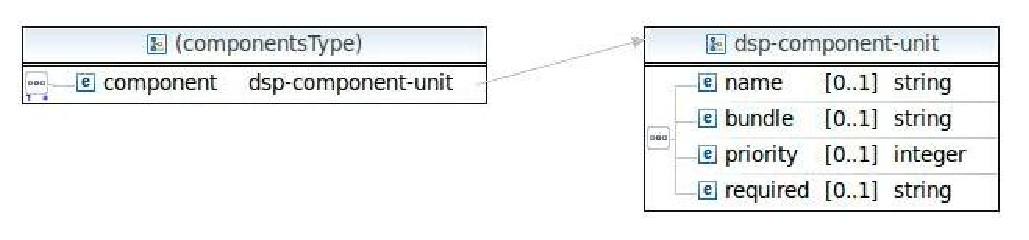
\includegraphics[scale=0.8]{../diagrams/config-schema}
  \caption{XML Schema for the main DSP deployment configuration artifact}
  \label{fig:dsp-config-schema}
\end{figure}

In order to show an example, consider the DSP Platform on the embedded system
Gumstix in figure \ref{fig:sf-netbeams-node}. It is started by providing a
deployment configuration artifact config.xml included in the appendix. It lists
the components that the DSP Platform needs to install and load for its
operation. As it is shown, the DSPWireTransportClient and the DSPSondeProducer
are the identification of the components, followed by the name of the physical
file and an assigned loading priority. While the DSPWireTransportClient is
responsible for the serialization and deserialization of the DSP Messages
exchanged by the DSPSondeProducer and any remote DSP component. In this case,
the DSPSondeProducer is the DSP component responsible to collect measurement
data from the YSI Sonde and temporarily store them before being transmitted.

Therefore, in order to orchestrate the DSP Components together, the DSP
Platform component is responsible for installing and uninstalling during its
state "Starting" and "Stopping", respectively, as it is shown in figure
\ref{fig:DSPPlatform-Install-Usage-State-Diagram}. When the system
administrator starts the DSP Platform, it performs the regular OSGi procedures
to start the bundle. Up until that state, it will get the list of DSP
Components to be installed as described in the config.xml artifact, trying to
install each of them in an optimistic way. After that, it will continue on the
state "Active" until the system administrator decides to stop it.

\begin{figure}[!b]
  \centering
  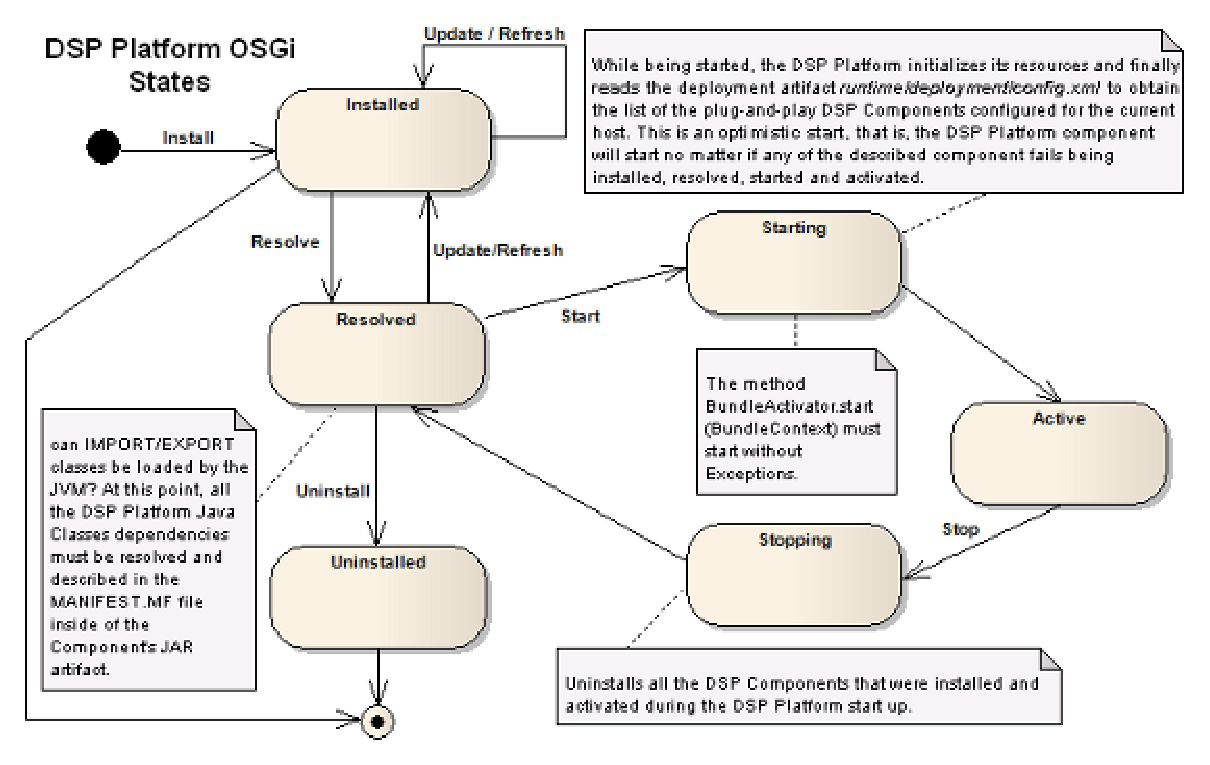
\includegraphics[scale=0.6]{../diagrams/DSPPlatform-Install-Usage-State-Diagram}
  \caption{The DSP Platform State Diagram}
  \label{fig:DSPPlatform-Install-Usage-State-Diagram}
\end{figure}

When the DSP Platform is on the Active state, it is ready to manage the DSP
Messages exchanges as described through figure
\ref{fig:DSP-Producers-Consumers-Components-Interactions}. The following
sections describe the participating classes in starting the DSP Platform and
its execution.

In a nutshell, the DSP Platform is an extension of the OSGi Platform, as it can
be seen in the UML Class Diagram \cite{uml} in figure
\ref{fig:DSP-Platform-Class-Diagram-Simple}. The class Activator contains a
unique instance of the Platform class, which contains instances of the classes
ComponentManager, Matcher, the MessageBroker and DSPContextImpl. The
DSPBundleController is the main instance that manages the plug-and-play DSP
components, and therefore, is tightly-coupled with the OSGi Framework classes.
Additionally, this class is part of the publish-subscriber design-pattern, as
it it implements the interfaces Bundle Listener and Service Listener, whose
responsibility is to track listens to the changes of the state of
ServicesReferences on the DSP Platform.

\begin{figure}[!t]
  \centering
  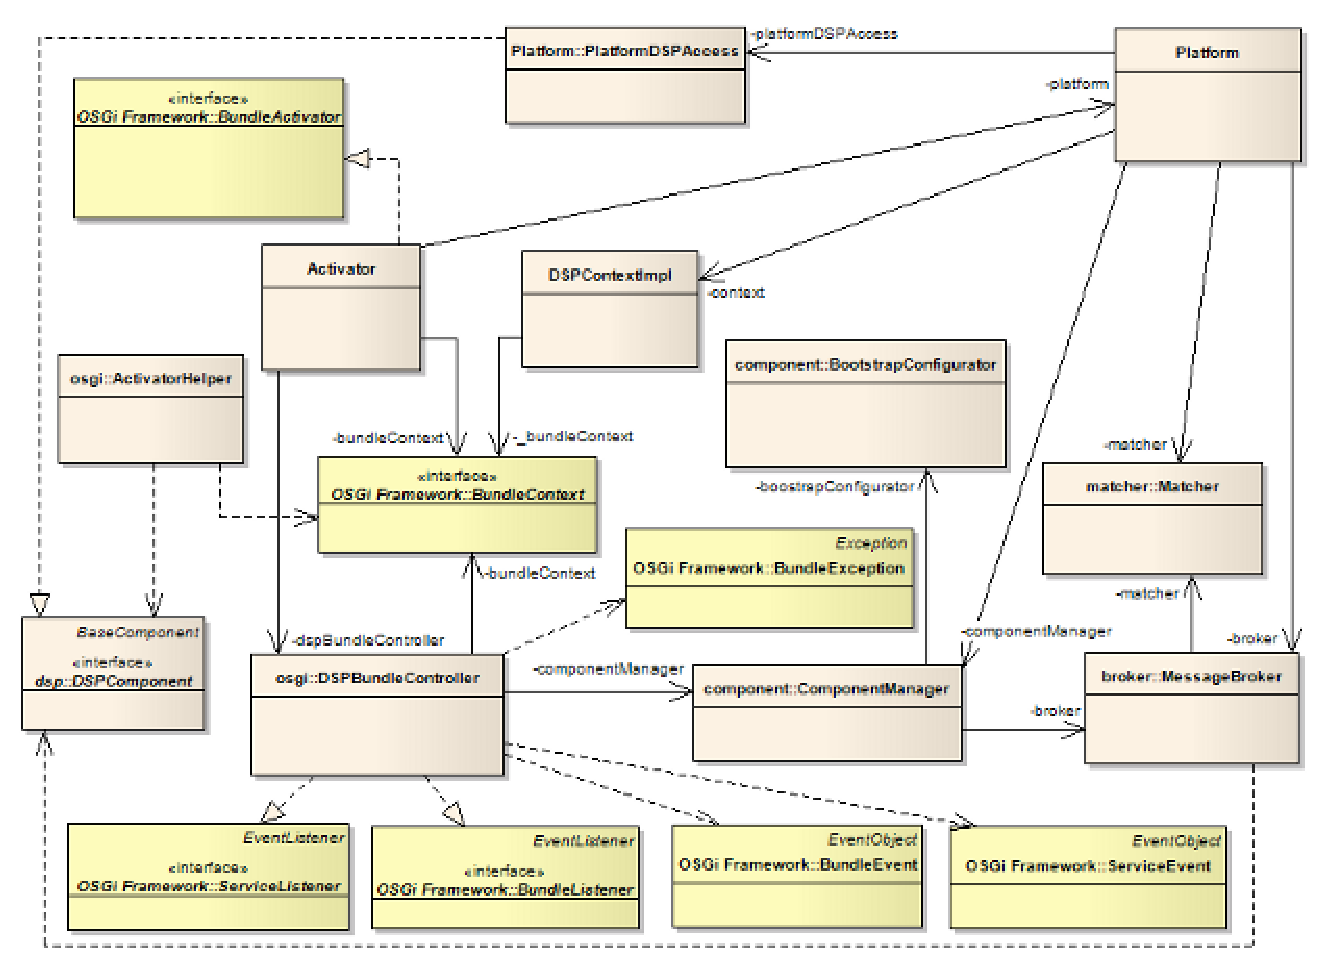
\includegraphics[scale=0.7]{../diagrams/DSP-Platform-Class-Diagram-Simple}
  \caption{The DSP Platform UML Class Diagram}
  \label{fig:DSP-Platform-Class-Diagram-Simple}
\end{figure}

\section{DSP Message and DSP Messages Container}
\label{sec:dsp-message}

As shown in the previous section, a DSP Message is the main unit of
communication among DSP Components. In a nutshell, a DSP Message can be seen
as an abstraction of an envelop containing the sections: a header and a body.
The former is used for identification and routing purposes, while the latter is
used to carry the payload of the message, that is, the collected data from
a sensor. Figure \ref{fig:DSP-Message-Representation} depicts the abstraction
of a DSP Message and its main components.

\begin{figure}[!b]
  \centering
  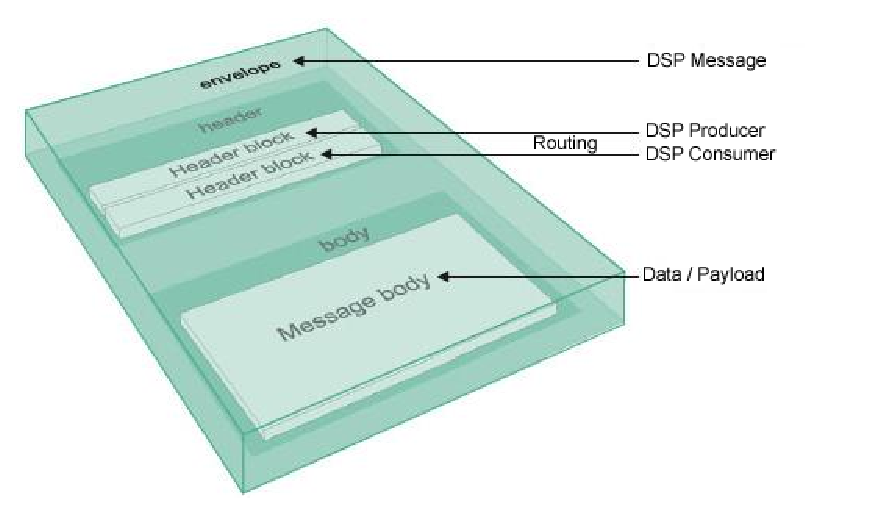
\includegraphics[scale=0.8]{../diagrams/DSP-Message-Representation}
  \caption{An Abstraction of a DSP Message and its components}
  \label{fig:DSP-Message-Representation}
\end{figure}

\begin{itemize}
  \item \textbf{Header} is composed by 2 blocks that identify the data
  producer and consumer of the message, as well as the time of creation, UUID,
  etc. It is an important piece of information for the data delivery and
  routing purposes.
  \item \textbf{Body} contains the payload of the message. This section carries
  the collected data from a sensor.
\end{itemize}

In general, the DSP Platform offers a veriety of types of DSP Messages for
different purposes. For example, any measurement data must be
wrapped up in a Measurement Message, while a Query Message is used to exchange
messages among the components for the purpose of management. In this way, the
main DSP Messages can be summarized as follows:

\begin{itemize}
  \item \textbf{Measurement Message} is used to transport any sensor collected
  data;
  \item \textbf{Query Message} is used to query a DSP component about its
  configuration properties;
  \item \textbf{Update Message} used to update a DSP component's configuration
  properties;
  \item \textbf{Acknowledgement Message} is used for the transport communication
  protocol, by acknowledging the reception of a DSP Message. More details in the
  Remote Data delivery section.
\end{itemize}

These DSP Classes and other can be seen in figure the  UML Class
Diagram \cite{uml} of figure \ref{fig:DSP-Messages-Classes}. Each DSP Message
contains an instance of a Header and Body. Whenever a DSP component is ready
to transmit messages, it wraps up the set of DSP Messages into the instance of
the Messages Container, which contains information about the collection of
messages being transmitted with its own identification. In this fashion, the
Messages Container is the main communication unit between 2 different DSP
Components.

\begin{figure}[!t]
  \centering
  \includegraphics[scale=0.6]{../diagrams/DSP-Messages-Classes}
  \caption{The DSP Messages UML Class Diagram}
  \label{fig:DSP-Messages-Classes}
\end{figure}

Another use of the DSP Messages is during the DSP Platform activation process,
where bootstrap messages are used to configure each DSP component. In order to
send configuration parameters, the DSP Platform uses Update Messages using a
unique type of Message Content called DSP Properties, which is described in the
next section.

\section{Collected Sensor Data as the DSP Message Content}
\label{sec:dsp-payload-implementation}

As mentioned in the previsou section, a DSP Message can carry any data on its
body, also called the payload. In such a way, any data representation must
just extend from the Message Content abstract class as it is shown
\ref{fig:Sonde-MessageContainer-Class-Diagram}, as defines the data
representation of the YSI Sonde data.

\begin{figure}[!h]
  \centering
  \includegraphics[scale=0.6]{../diagrams/Sonde-MessageContainer-Class-Diagram}
  \caption{The YSI Payload - Message Content UML Class Diagram}
  \label{fig:Sonde-MessageContainer-Class-Diagram}
\end{figure}

The properties measured from the YSI Sonde can be captured by the class
SondeDataType as a direct render of the measurements data depicted in table
\ref{tab:ysi-data-stream}. In addition to the regular data types, the class
also provides additional properties such as the attribute "samplingTimeStamp"
that carries the time when the data was collected from the YSI Sonde. However,
in order to capture a set of measurements at once, the SondeDataContainer
class used to carry a set of SondeDataType classes, as it is composed by one
or more instances of SondeDataType. In order to illustrate other examples,
consider the UML Class Diagram \cite{uml} of image
\ref{fig:Mouse-Actions--MessageContainer-Class-Diagram} as a payload of
observations made from a mouse over a screen, which captures the name of the
event, the button name and the x/y coordinates.

\begin{figure}[!h]
  \centering
  \includegraphics[scale=0.5]{../diagrams/Mouse-Actions--MessageContainer-Class-Diagram}
  \caption{The Mouse Actions Payload - Message Content UML Class Diagram}
  \label{fig:Mouse-Actions--MessageContainer-Class-Diagram}
\end{figure}

As described in the previous section, the DSP Platform uses DSP Update
Messages to configure internal components' initial configuration values. In
order to do so, the DSP Platform uses an instance of the DSP Properties, which
is composed of a list of initial DSP Property and their relating Values
instance depicted on the UML class diagram \cite{uml} of figure
\ref{fig:DSP-Property-Class-Diagram}. 

\begin{itemize}
  \item \textbf{Property Instance}: initial-rate
  \item \textbf{Value Instance}: 40
\end{itemize}

\begin{figure}[!t]
  \centering
  \includegraphics[scale=0.6]{../diagrams/DSP-Property-Class-Diagram}
  \caption{The DSP Property Payload - Message Content UML Class Diagram}
  \label{fig:DSP-Property-Class-Diagram}
\end{figure}

\subsection{DSP Platform Initialization Process}

All in all, the DSP Platform requires the knowledge of the aforementioned DSP
classes in order to initialize. The UML Sequence Diagram \cite{uml} in figure
\ref{fig:From-OSGi-DSP-Platform-Start-to-All-Components-Sequence-Diagram}
depicts the exact moments when the additional the plug-and-play DSP components
are installed and bootstrapped by the DSP Platform, as the UML State Diagram
\cite{uml} in figure \ref{fig:DSPPlatform-Install-Usage-State-Diagram}
described.

\begin{itemize}
  \item \textbf{Start DSP Activator Gate}: after installing the Activator
  indicated by the DSP Bundle's MANIFEST.MF artifact, the OSGi Framework makes
  a call to the method Activator.start();
  \item \textbf{Bootstrap DSP Component Gate}: after the component has been
  initialized (by the call the method init() from the class ComponentManager),
  the DSP Component is ready to be bootstrapped, and the optional bootstrap
  message is delivered.
\end{itemize}

\begin{figure}[!b]
  \centering
  \includegraphics[scale=0.5]{../diagrams/From-OSGi-DSP-Platform-Start-to-All-Components-Sequence-Diagram}
  \caption{The DSP Platform Initialization UML Sequence Diagram}
  \label{fig:From-OSGi-DSP-Platform-Start-to-All-Components-Sequence-Diagram}
\end{figure}

\newpage

\subsection{Data Delivery Mechanism}

In general, when a DSP Component finishes preparing the DSP Messages Container,
it contacts an entity responsible for sending and proxying message to other
components. The DSP Broker acts like a mailman, receiving messages and
forwarding copies of it to other entities in the system, abstraction in which
is shown in figure \ref{fig:DSP-Message-Broker-Abstraction}. In this way, the
DSP Broker receives a DSP Message and makes necessary deliveries to DSP
components that it has knowledge of.

\begin{figure}[!h]
  \centering
  \includegraphics[scale=0.8]{../diagrams/DSP-Message-Broker-Abstraction}
  \caption{A DSP Message Broker Abstraction}
  \label{fig:DSP-Message-Broker-Abstraction}
\end{figure}

The use of messaging exchange paradigm is used in NetBEAMS because it decouples
the system by using messages take into account their structure to filter the
messages. In this way, the DSP Broker uses a filter component called DSP
Matcher, which provides a list of DSP Components that needs to receive a copy
of the DSP Message. It turns out that the DSP Matcher bases its decisions on
structured rules provided by the system administrator for an specific DSP
Platform instance. The UML Class diagram for the DSP Broker, Matcher and
particiaping classes is depicted in figure
\ref{fig:DSPBroker-Matcher-Class-Diagram}, and describes how the DSP Broker
implementation is tightly coupled with the DSP Matcher, as well as to the
lists of DSP Components sorted by name and type.

\begin{figure}[!b]
  \centering
  \includegraphics[scale=0.6]{../diagrams/DSPBroker-Matcher-Class-Diagram}
  \caption{The DSP Broker-Matcher UML Class Diagram}
  \label{fig:DSPBroker-Matcher-Class-Diagram}
\end{figure}

In general, the DSP Matcher is composed by a list of MatchRule, which contains
a reference to a MatchCriteria and a MatchTarget. The former identifies the
rule for matching a given DSP Message based on the producer and consumer's
message type and location, while the latter describes the DSP Component that
will receive the DSP Message, and if its delivery is done by means of a gateway
component. In this way, the DSP Matcher can be seen as a function that takes a
DSP Message as an input and returns a list of DSP consumers, and the
matching configuration artifact provided by the administrator. See listing
\ref{file:dsp-matcher-config.xml}) for details.

\begin{table}
    \caption{DSP Matcher Rule Algorithm to filter Data Consumer components to
    receive a given Message}
    \begin{center}
        \begin{tabular}{lr}
          \textit{Data Consumers ( DSP Message )} := \\ 
          Verify the DSP Message's Header + \\
          Verify the matcher rules, which contains the list of consumers for
          the given message
        \end{tabular}
    \end{center}
    \label{tab:ysi-data-stream}
\end{table}

One example of such matching rule used by the DSP installed at the Gumstix can
be seen in listing \ref{file:dsp-matcher-config-gumstix.xml}. the Gumstix
system to configure the data delivery of the messages produced by the DSP
Component DSP Sonde Producer. It describes a list of maching rules that
reseambles a filtering system. This configuration contains 2 match rules: one
related to internal DSP Configuration and another for a remote destination.
The match criteria describes what the DSP Message Header properties must be,
while the match target is the destination of the message. One important
definition is the gateway Component Type, which defines the name of a remote
DSP Component that is capable of receiving a remote DSP Message.

Upon receiving all the matching rules and analyzing the DSP Message against
the rules, the DSP Broker selects a set of the running DSP components to receive
a copy of the DSP Message object in two different ways:

\begin{itemize}
  \item \textbf{In-memory local message delivery}: if the receiving DSP
  Component is located in the current local host, a deep copy of the instance
  of the DSP message is delivered;
    \begin{itemize}[label=\textbullet]
        \item IP Addresses are correctly resolved by using the Ethernet card in
        the device: localhost, 127.0.0.1, or the same IP Address for Producer
        and Receiver resolves into a local device. An example for such type of
        delivery can be seen in the match ruleID
        all messages sent to dsp manager of listing 
        \ref{file:dsp-matcher-config-gumstix.xml}.
    \end{itemize}
  \item \textbf{Serialized remote message delivery}: if the receiving DSP
  Component is located in a foreign/remote host, the message is serialized in a
  format defined by the transport protocol chosen the DSP Component responsible
  for the transport. The following section describes the existing DSP Data
  Transport component;     
  \begin{itemize}[label=\textbullet]
        \item IP Address from the Producer and Consumer are different, and are
        not resolved to be in the same host. An instance of such match rule can
        be seen in the match rule ID send-message-to-remote url dsp of the code
        snippet \ref{file:dsp-matcher-config-gumstix.xml}.
    \end{itemize}
\end{itemize}

\subsection{Sending DSP Messages through the Wire}

In order to send messages through the wire, the DSP Platform uses two symmetric
components that serialize and deserialize DSP Messages to XML and back to Java
POJO, respectively, and vice-versa. Named DSP Wire Transport Client and DSP
Wire Transport Server \cite{netbeams2009}, these components use the HTTP
\cite{http} protocol to transport the serialized version of the DSP Messages.
Figure \ref{fig:DSP-to-DSP-Remote-Communication} depicts the scenario where a
DSP Sensor Node transmits a DSP Message through an HTTP POST request.

\begin{figure}[!b]
  \centering
  \includegraphics[scale=0.6]{../diagrams/DSP-to-DSP-Remote-Communication}
  \caption{The remote communication between two DSP Components using the HTTP
  Protocol}
  \label{fig:DSP-to-DSP-Remote-Communication}
\end{figure}

\begin{itemize}
  \item \textbf{DSP Wire Transport Client}: responsible for making HTTP POST
  Requests to the service provided by the DSP Wire Transport Server component.
  The body of the HTTP POST request contains a serialized version of an
  instance of a DSP MessagesContainer in XML format;
  \item \textbf{DSP Wire Transport Server}: exposes a Web Server listening to
  port 8080 that receives the HTTP POST request from the Client. Upon receiving
  the request, the server deserializes the DSP MessagesContainer back to the
  in-memory POJO and proceeds with the delivery to the DSP Broker. At this
  situation, the component packages acknowledgement messages and any queued
  message to the client and piggybacks \cite{xml-piggybacking} it to the HTTP
  response body.
\end{itemize}

As described by \cite{netbeams2009}, NetBEAMS is a single-hop sensor network
whose sensors transmits data from the sensors to the server. Upon receiving the
data stream, the DSP Wire Transport Server component desirializes the DSP
MessagesContainer and its enclosing DSP Messages back to a Java class instance
and delivers each of the DSP Messages to the DSP Broker, which delivers a
copy of the message to each DSP Component listed by the maching rule. 
%This
%process is depicted by the UML Sequence Diagram \cite{uml} in figure \ref{fig:}

Whenever a DSP bundle producer is ready to transmit messages, they are added
into a DSP Messages Container (see UML Class Diagram in figure
\ref{fig:DSP-Messages-Classes}), which is serialized in XML to be transmitted.
Listing \ref{file:dsp-message-serialized-ysi} shows an instance of a DSP
MessagesContainer in serialized in XML, ready for transmission. In fact, the
listing is an example of the transmitted data collected from a sensor located
at the 192.168.0.103 to be transmitted to the host 192.168.0.106, and the
process of transmission in the server-side can be followed in figure
\ref{fig:From-DSPSondeComponent-to-DSPWireTransportClient-Sequence}.

\begin{figure}[!h]
  \centering
  \includegraphics[scale=0.5]{../diagrams/From-DSPSondeComponent-to-DSPWireTransportClient-Sequence}
  \caption{The UML Sequence Diagram for the production of a YSI Message}
  \label{fig:From-DSPSondeComponent-to-DSPWireTransportClient-Sequence}
\end{figure}

The Sonde DSP Component is responsible for starting a worker thread called
SondeProducer, which is responsible for constantly read from the RS-232 serial
port by using an instance of the SerialReader class. This process depicts the
production of the data flow "flow 1" of figure
\ref{fig:netbeams-software-stack}, which is a collection of SondeDataType for
each of the measurement data read on a SondeDataContainer. As depicted in
figure \ref{fig:From-DSPSondeComponent-to-DSPWireTransportClient-Sequence}, it
first read the serial connection using the class SerialReader, which parses 
the data stream. After parsing the data, the reader creates an instance of the
class SondeDataType, the POJO responsible for carrying out the measurement
data. As described earlier, the data is added into the SondeDataContainer to
dispatched to the DSP Broker, whose responsibility is to get the list of DSP
Components that is setup to receive a copy of the DSP message (see previous
code snippet). As for the setup done for the Gumstix, the measurement message
is supposed to be sent to a remote destination of host 192.168.0.7. At this
point, the DSP Broker makes a decision to send the DSP Message to the default
gateway component DSPWireTransportClient.

After the message arrives in the DSPWireTransportClient, the message is
maintained in a temporary repository of outbound DSP Messages called
MessagesQueues after the message is hashed by the destination IP address and
the DSP Client sender using an instance of QueueMessageData. As shown in figure
\ref{fig:From-DSPWireTransport-Client-to-DSPWireTransportServer-Sequence}, the
DSP TransportSender is a worker thread that is started by the DSP Wire
Transport Client and is constantly transmits the data in the outbound queues
after a configurable rate. It makes a transport of the message and receives
the response, updates the state of the messages to transmitted, to finally
send the response messages to the DSP Message Broker.

\begin{figure}[!t]
  \centering
  \includegraphics[scale=0.5]{../diagrams/From-DSPWireTransport-Client-to-DSPWireTransportServer-Sequence}
  \caption{The UML Sequence Diagram describing the Wire Transport Server
  receiving a DSP Message}
  \label{fig:From-DSPWireTransport-Client-to-DSPWireTransportServer-Sequence}
\end{figure}

While the DSPWireTransportClient makes an HTTP Request with the DSP Message,
the DSPWireTransportServer's servlet receives the request. It first
deserializes the MessagesContainer and delivers each of its messages to the DSP
Broker. At this point, the server verifies if there are messages in the
outbound queue that are addressed for the host that requested the messages
delivery. By using a technique called piggybacking, the server adds to the HTTP
Response a serialized version of the MessagesContainer with any DSP Messages.
In addition to any DSP Message, the server prepares and sends acknowledgement
messages back to the requesting host to the host.

\begin{figure}[!t]
  \centering
  \includegraphics[scale=0.5]{../diagrams/From-DSPWireTransport-Server-To-DSP-Broker}
  \caption{The UML Sequence diagram describing the DSP
Message delivery on the server-side and the response}
  \label{fig:From-DSPWireTransport-Server-To-DSP-Broker}
\end{figure}

The gate "From DSP WireTransport Server to Broker Gate" defines the actual
delivery of the DSP Message to the DSP Broker. As this section is a tutorial
about the DSP Platform, the remaining steps will be explained on Section 3,
while showing the design and implementation of the component DSP Data
Persistence.

\section{DSP Data Persistence: Component Implementation}
\label{sec:dsp-data-persistence-implementation}

This section shows the implementation of the DSP Data Persistence, which
follows the specifications of the DSP Components in the previous chapter,
along with the setup of the mongoDB, the chosen database system that models
data in a type of key-value pair model. Moreover, this chapter also describes
the experiments conducted for the persistence.

The implementation of the DSP Data Persistence component, as well as the
implementation of the experiments, were developed and managed using the DSP a
reserved development branch at the Subversion \cite{subversion} repository
located at the Google Code website. In this way, anyone can checkout the entire
source-code from the branch
\textit{https://netbeams.googlecode.com/svn/branches/marcello/persistence},
as shown in Figure \ref{fig:dsp-data-persistence-dir}. In this way, the
recommended checkout branch directory will give the remaining directory
structure as summarized:

\begin{itemize}
  \item \textbf{NEBEAMS-DIR/}: the directories under the subdirectory
  ``persistence'';
  \item \textbf{DEV-VERSION}: the directory of the current development
  version for the DSP; That is, ``\textbf{NEBEAMS-DIR}/versions/v2/''
  \item \textbf{PERSISTENCE-DIR}: the directory of the DSP component, that is,
  ``\textbf{DEV-VERSION}/apps/osgi-intro-bundles/dsp/DSPDataPersistence''.
\end{itemize}

\begin{figure}[!b]
  \centering
  \includegraphics[scale=0.6]{../diagrams/dsp-data-persistence-dir}
  \caption{The DSP Data Persistence Directory Structure}
  \label{fig:dsp-data-persistence-dir}
\end{figure}

The DSP Platform defines its own run-time directory, which organizes the
artifacts used by the osgi-intro Framework, as well as the its own configuration
descriptor and matcher, as described in the previous section. 

\begin{itemize}
  \item \textbf{RUNTIME-DIR}: the main directory for the execution of the DSP
Platform, with all the necessary osgi-intro-related artifacts are placed, as shown in
Figure \ref{fig:dsp-runtime-dir}.
\end{itemize}

\begin{figure}[!t]
  \centering
  \includegraphics[scale=0.5]{../diagrams/dsp-runtime-dir}
  \caption{The DSP Data Persistence Directory Structure}
  \label{fig:dsp-runtime-dir}
\end{figure}

\section{DSP Platform Deployment Details}

As described in the previous chapter, the DSP Data Persistence Component was
implemented using the Java Programming language, on top of the osgi-intro Framework
API. This section describes the setup process of the implementation, as well as
the artifacts use during the implementation, which will be listed in the
appendix section.

The structure of the artifacts implemented for the DSP Data Persistence
Component follow the conventions of the NetBEAMS implementation, where the main
directory \textbf{PERSISTENCE-DIR}, depicted by Figure
\ref{fig:dsp-data-persistence-dir-checkedout}, holds each of the development
artifacts.

\begin{itemize}
  \item \textbf{DSPDataPersistence}: Main directory with the build.xml (Listing
  \ref{file:dsp-build.xml}) and other Eclipse-related artifacts. The other
  major directories are also listed:
  \item \textbf{META-INF}: this directory contains the descriptor file for
  the osgi-intro Framework, this this case the MANIFEST.MF;
  \item \textbf{src}: the main directory structure for the source-code
  implemented. Note that it follows the Java specification for packaging, and
  therefore, lists the package org.netbeams.dsp.persistence as the main
  package, including the layers controller, model and osgi-intro.
\end{itemize}

\begin{figure}[!h]
  \centering
  \includegraphics[scale=0.5]{../diagrams/dsp-data-persistence-dir-checkedout}
  \caption{The DSP Data Persistence Directory Structure}
  \label{fig:dsp-data-persistence-dir-checkedout}
\end{figure}

\subsection{osgi-intro Deployment Process}

Since each NetBEAMS component is managed by an osgi-intro component and its
infrastructure, this section describes the basic functionality of the osgi-intro
platform \cite{osgi-intro}, a framework was conceived to support modularity in
terms resources-limited environments such mobile devices and vehicles, but it
was first widely deployed on Eclipe IDE\footnote{Integrated Development
Environment}, because it promotes the use of reusable loosely-coupled modules
using the Java Programming Language \cite{java}. The most basic layer of the
osgi-intro Framework depicted in Figure \ref{fig:layering-osgi-intro} are as follows:

\begin{itemize}
  \item \textbf{Module Layer}: manages the osgi-intro bundles deployed on the osgi-intro
  Platform, providing the necessary "wiring" of the components. In other words,
  the modules, called osgi-intro Bundles, can export and/or import packages in the
  level of a Java Class managed by the osgi-intro Framework;
  \item \textbf{Service Layer}: resposible for the interoperability between 2
  or more bundles, enabling the bundles to register services offered by
  the its specification;
  \item \textbf{Execution Layer}: executes the bundles, managing and changing
  their life-cycle through the bundle execution.
\end{itemize}

\begin{figure}[!h]
  \centering
  \includegraphics[scale=0.5]{../diagrams/layering-osgi}
  \caption{The osgi-intro Framework Layers}
  \label{fig:layering-osgi-intro}
\end{figure}

NetBEAMS uses the concept of the modularization through the use of the the
Producer-Consumer paradigm described in the previous section. Since the DSP
Components are essentially osgi-intro bundles, the interoperability between them are
given in the implementation and reuse existing bundles in the osgi-intro Framework
and the DSP Platform, described by an artifact called MANIFEST.MF as seen in
Listing \ref{file:osgi-intro-manifest}. In general, an osgi-intro bundle must
provide specifications that describes the module to be published into the osgi-intro
Framework. In this way, the main properties of the osgi-intro MANIFEST.MF artifact can
used by the DSP Data Persistence can be summarized as follows:

\begin{itemize}
  \item \textbf{Bundle-Activator}: The name of the instance of an osgi-intro Activator
  class, responsible to manage the bundle. The implemented class
  ``DataPersistenceActivator'' provides the activation mechanisms for the
  services provided by the DSP Data Persistence Component;
  \item \textbf{Bundle-ClassPath}: the necessary Java Jars list needed to run
  the bundle. It lists the mongoDB Java driver as one of the required
  dependencies deployed in the same package;
  \item \textbf{Import-Package}: the Java Packages needed by the DSP Data
  Persistence Component Bundle. These Java Packages must be provided by other
  DSP components, forcing the execution to be dependent on those package.
  They are provided through a ``Export-Package'' section in other osgi-intro
  bundles and, as it is shown in Listing \ref{file:osgi-intro-manifest}, they
  are from different packages.
\end{itemize}

Once the osgi-intro bundle is installed into the osgi-intro Platform, it will be managed by
the osgi-intro Execution layer and change the bundle state according to its
lify-cycle, as described in the previous chapter. Therefore, the packaging of
the osgi-intro source-code is done using a JAR\footnote{Java Archival Repository}
artifact specification \cite{java-tutorial}. In this way, the DSP Data
Platform osgi-intro bundle JAR is created by the Apache ANT build script
\cite{apache-ant} in Listing \ref{file:dsp-build.xml}. The task
``dsp-data-persistence.all'' compiles all the source-code created from the
design of the previous chapter and packages everything into the artifact
``DSPDataPersistence-x.x.jar'', where x.x is the version of the bundle. Figure
\ref{fig:dsp-runtime-dir} shows the DSP Data Persistence file under the
dirctory ``\textbf{RUNTIME-DIR}/deployment/''.

\subsection{Adding DSP Data Persistence into DSP Platform }

Once the new component was developed, the DSP Data Persistence component was
deployed by editing two main descriptors, as well as the optional bootstrap
message, as described in chapter 5:

\begin{itemize}
  \item \textbf{config.xml}: the DSP Data Persistence is added to the DSP
  Platform adding an entry for the component;
  \item \textbf{matcher\underline{ }config.xml}: the addition of the rules that
  filters the messages to the DSP Data Persistence;
  \item \textbf{DSPDataPersistence\underline{ }001.xml}: depicts the bootstrap
  message for the DSP Data Persistence Component, as shown in Listing 
  \ref{file:dsp-data-persistence-bootstrap.xml}.
\end{itemize}

The first configuration artifact enables NetBEAMS to initialize contain the
descriptor of the component, as shown in Listing \ref{file:dsp-config.xml}.
The component is added with the highest priority, since it contains
dependencies to other DSP Components. 
\subsection{Starting the DSP Platform}

Once the DSP Platform automatically installs all the components described by
the configuration descriptor, the container verifies the dependencies and
starts each of the DSP components of Figure \ref{fig:knopflerfish-execution},
the osgi-intro Framework container Knopflerfish \cite{knopflerfish}.

\begin{figure}[!t]
  \centering
  \includegraphics[scale=0.65]{../diagrams/knopflerfish-execution}
  \caption{The execution of the Knopflerfish Container}
  \label{fig:knopflerfish-execution}
\end{figure}

\subsection{Execution Logs}

\section{mongoDB Deployment}

Given that Document-Oriented Model makes a good candidate persist sensors'
properties and the recently enumerated list technologies in the previous
article DSPDataPersistence, the open-source project called mongoDB was chosen
for the evaluation on our case study, the netBEAMS DSP Platform.

mongoDB supports storage based on collections of data, stored using BSON, a
binary representation the JSON data representation format, including dynamic
queries and indexing support. As it's stated in their web site, mongoDB
"bridges the gap between key/value stores (which are fast and highly scalable)
and traditional RDBMS systems (which are deep in functionality)".

\begin{itemize}
  \item mongoDB implements a document-oriented structure, which is similar to
  KVP;
  \item mongoDB is written in C++, and therefore, can is available in any major
  platform, as well as offers a broad range of API drivers written in different
  languages such as Java, Python, Perl and Ruby; 
  \item mongoDB is open-source, with good community support and availability
  through mailing lists, freenode IRC channel, and commercial support through
  10gen company; 
  \item mongoDB has support to distributed systems properties such as
  Master-Slave replication, and features like Database Shards with
  auto-sharding based on shard keys.
\end{itemize}

The artifacts of the mongoDB are located in the thirdparty directory of the
NetBEAMS resources. However, the build script from the DSP Data Persistence
component can be executed to produce the persistence directory
structure for NetBEAMS, as described in figure
\ref{fig:dsp-persistence-system-dir}.

\begin{figure}[!h]
  \centering
  \includegraphics[scale=0.5]{../diagrams/dsp-persistence-system-dir}
  \caption{The osgi-intro Framework Layers}
  \label{fig:dsp-persistence-system-dir}
\end{figure}

\subsection{Document-Oriented Data Model}

An example of the data is as folows (using the JSON syntax). Listing
\ref{file:mongodb-ysi-data-format} follows the strategy described on Section X,
where the entity representation is denormalized, and each of the properties of
the sensor is repeated in each instance of the data. The fact and transaction
times are expressed in milliseconds. The data element contains the complete
structure of the originating sensor such as the IP address. The collection of
instances of this document represents the sensor data type.

\subsection{Starting the Database}

\subsection{Stopping the Database}

\subsection{Execution Logs}

\section{Experiment Execution}

The experiments conducted using mongoDB can be summarized by the different
data access methods provided by the technology. Each subsection describes these
methods.

\subsection{Data Access Using Database Shell}

The mongoDB client can be started by using the following command. Make sure you
have started the mongoDB server before executing the mongoDB client.

mongo netbeams | tee output\underline{ }number\underline{ }date.log

Here, the iterative mongo client shell offers users to verify and navigate on a
given database and its collections. This first section shows the connection of
the mongo client to the database netbeams. It also highlights the query for the
collections available. During the experiment, the SondeDataContainer?
collection was created as related to the type from the DSP Messages for the YSI
Sonde.

The shell references to the mongoDB system can be found at
http://www.mongodb.org/display/DOCS/dbshell+Reference 

\lstset{label=cmd:mongo,caption=Execution of mongo client}
\begin{lstlisting}
MongoDB shell version: 1.1.0-
url: netbeams
connecting to: netbeams
type "help" for help
> show collections
SondeDataContainer
system.indexes
>
> db.SondeDataContainer.count()
1000000
\end{lstlisting}

Then, the first verification of the data integrity is regarding the number of
elements created. Here, the first count() function on the collection returned
1000000.

An example about retrieving the first element of the collection can be done
using the findOne() function. It will return an element instance on the
JSONnotation.

\lstset{label=cmd:mongo-findone,caption=Querying the database: one item}
\begin{lstlisting}
> db.SondeDataContainer.findOne()
{
    "_id" : ObjectId("5d6f40078ec8074bba980900"),
    "message_id" : "020d82e1-18b2-4fe2-800c-a0f68e22ea86",
    "sensor" : {
        "ip_address" : "192.168.0.91",
        "location" : {
            "latitude" : 37.89155,
            "longitude" : -122.4464
        }
    },
    "time" : {
        "valid" : "Wed Nov 04 2009 02:30:12 GMT-0800 (PST)",
        "transaction" : "Sat Nov 21 2009 03:01:33 GMT-0800 (PST)"
    },
    "observation" : {
        "WaterTemperature" : 88.58,
        "SpecificConductivity" : 180.5,
        "Conductivity" : 167.3,
        "Resistivity" : 491.89,
        "Salinity" : 0.06,
        "Pressure" : 1.109,
        "Depth" : 2.642,
        "pH" : 7.11,
        "pHmV" : -42.9,
        "Turbidity" : 0.2,
        "ODOSaturation" : 72.4,
        "ODO" : 10.85,
        "Battery" : 2.7
    }
}
\end{lstlisting}

The query based on attributes can be done using the "dot" notation, as you
navigate through the JSON documents. Additionally, you can use the functions as
aggregated on the result of others. The example in listing
\ref{cmd:mongo-find-list} counts the number of documents with the key
"data.ph" equals to "5.64".

\lstset{label=cmd:mongo-find-list,caption=Execution of mongo client}
\begin{lstlisting}
> db.SondeDataContainer.find({"data.ph":5.64)}).count()
1226
\end{lstlisting}

The following example is the output of the first 2 documents from the same
previous query using the limit() function, as shown in figure
\ref{cmd:mongo-find-limit}.

\lstset{label=cmd:mongo-find-limit,caption=Query Element with specific
projection limiting the result set size}
\begin{lstlisting}
> db.SondeDataContainer.find({"data.ph":5.64}).limit(2)
{"_id" :  ObjectId( "d36f4007b7e7ac4a03c60000")  , "sensor_ip_address" : "192.168.0.136" , "message_id" : "7b6624d6-0ca1-4cba-a343-f166e88da73b"
, "transaction_time" : 1252845473412 , "fact_time" : 1252845346000 , "data" : {"temperature" : "45.01" , "sp_condition" : "37.6" ,
"condition" : "145.8" , "resistence" : "159.77" , "salinitude" : "0.0" , "pressure" : "0.391" , "depth" : "0.46" , "ph" : "5.64" ,
"pH_mv" : "-62.1" , "odo_sat" : "89.7" , "odo_condition" : "59.34" , "turbidity" : "0.0" , "battery" : "9.4"}}
{"_id" :  ObjectId( "d36f4007b7e7ac4a1fc80000")  , "sensor_ip_address" : "192.168.0.136" , "message_id" : "7b6624d6-0ca1-4cba-a343-f166e88da73b" ,
"transaction_time" : 1252845473412 , "fact_time" : 1252845346000 , "data" : {"temperature" : "46.71" , "sp_condition" : "60.8" ,
"condition" : "160.6" , "resistence" : "1399.4" , "salinitude" : "0.01" , "pressure" : "1.057" , "depth" : "2.485" , "ph" : "5.64" ,
"pH_mv" : "-16.3" , "odo_sat" : "58.8" , "odo_condition" : "19.29" , "turbidity" : "0.2" , "battery" : "9.2"}}
>
\end{lstlisting}

Other logs are located at
http://code.google.com/p/netbeams/downloads/list

\subsection{Data Access Using APIs}

The mongoDB server offers different drivers to access the data, as well as the
Web Services.

\begin{itemize}
  \item The Java tutorial on the drivers is located at
    http://www.mongodb.org/display/DOCS/Java+Tutorial. The driver is located on
    the NETBEAMS/versions/v2/thirdparty/mongodb directory;  
  \item The REST API can be called from any HTTP client. At the time of the
  editing, this feature is still under alpha version. Check the documentation
  athttp://www.mongodb.org/display/DOCS/Http+Interface for details 
\end{itemize}

The following HTTP GET Request method returns the first 5 documents in the collection:
http://127.0.0.1:28017/netbeams/SondeDataContainer/?limit=-5, as shown in
listing \ref{cmd:mongo-rest-request}.

\lstset{label=cmd:mongo-rest-request,caption=REST HTTP GET Request Example}
\begin{lstlisting}
HTTP/1.0 200 OK
x-action:
x-ns: netbeams.SondeDataContainer
Content-Type: text/plain;charset=utf-8

{
  "offset" : 0,
  "rows": [
    { "_id" : "156f4007e4c3b74a36ed3100", "sensor_ip_address" : "192.168.0.117", "message_id" : "08b02c08-9290-4517-9a28-c6ee7e16509a",
"transaction_time" : 1253557219486, "fact_time" : 1253557217000, "data" : { "temperature" : "31.44", "sp_condition" : "99.8", "condition" : "53.5",
"resistence" : "1157.08", "salinity" : "0.0", "pressure" : "1.066", "depth" : "0.161", "ph" : "1.08", "pH_mv" : "-82.0", "odo_sat" : "40.3",
"odo_condition" : "56.85", "turbidity" : "0.2", "battery" : "8.2" } } ,
    { "_id" : "156f4007e5c3b74a37ed3100", "sensor_ip_address" : "192.168.0.117", "message_id" : "08b02c08-9290-4517-9a28-c6ee7e16509a",
"transaction_time" : 1253557219486, "fact_time" : 1253557217000, "data" : { "temperature" : "37.83", "sp_condition" : "176.3", "condition" : "2.6",
"resistence" : "1324.97", "salinity" : "0.01", "pressure" : "1.36", "depth" : "1.564", "ph" : "0.12", "pH_mv" : "-23.5", "odo_sat" : "104.5",
"odo_condition" : "19.44", "turbidity" : "0.1", "battery" : "5.0" } } ,
    { "_id" : "156f4007e5c3b74a38ed3100", "sensor_ip_address" : "192.168.0.117", "message_id" : "08b02c08-9290-4517-9a28-c6ee7e16509a",
"transaction_time" : 1253557219486, "fact_time" : 1253557217000, "data" : { "temperature" : "74.3", "sp_condition" : "84.0", "condition" : "104.7",
"resistence" : "4089.13", "salinity" : "0.01", "pressure" : "1.222", "depth" : "2.788", "ph" : "6.56", "pH_mv" : "-78.1", "odo_sat" : "40.0",
"odo_condition" : "6.02", "turbidity" : "0.3", "battery" : "3.2" } },
  "total_rows" : 3 ,
  "query" : {} ,
  "millis" : 0
}
\end{lstlisting}

Data visualisation tools for mongoDB is slowly being developed by open-source
developers. The next picture shows the database "netbeams" and the collection
"SondeDataContainer  ?" being rendered by futon4mongodb, one of the
open-source tools developed to visualise mongoDB data.

\subsection{Visualizing Data on The Browser}

Futon4Mongo is an open-source software adapted from CouchDB \cite{couchdb}.
First, the collections list is shown. Figure
\ref{fig:view-collections-instance-browser-futondb} shows one single collection
for the YSI data containing 1 million objects.

\begin{figure}[h]
  \centering
  \includegraphics[scale=0.5]{../diagrams/view-collections-instance-browser-futondb}
  \caption{Viewing a partial list of data using the Futon for CouchDB/MongoDB}
  \label{fig:view-collections-instance-browser-futondb}
\end{figure}

The collection is composed by instances of documents of representing the YSI
Sonde type, being indexed by a document ID and the values being the keys
defined in the previous chapter, as shown in figure
\ref{fig:view-collected-data-list-browser-futondb}.

\begin{figure}[h]
  \centering
  \includegraphics[scale=0.5]{../diagrams/view-collected-data-list-browser-futondb}
  \caption{Viewing a partial list of data using the Futon for CouchDB/MongoDB}
  \label{fig:view-collected-data-list-browser-futondb}
\end{figure}

By clicking in one of the items, one can view the instance of the document, as
it is shown in figure \ref{fig:view-collections-instance-browser-futondb}.

\begin{figure}[h]
  \centering
  \includegraphics[scale=0.5]{../diagrams/view-collected-data-instance-browser-futondb}
  \caption{Viewing an instance of collected data using the Futon for
  CouchDB/MongoDB}
  \label{fig:view-collected-data-instance-browser-futondb}
\end{figure}

\subsection{Exporting Data to Spreadsheets}

mongoDB has an export facility shell called mongoexport. It can export the data
in JSON format or CSV. One may also write its own export tool in any of the
languages such as Java, PHP, Python, Perl, Ruby, among others. A list of the
existing drivers in different languages is provided
athttp://www.mongodb.org/display/DOCS/Drivers. The following command can be
executed to have the exported version of the data in CSV (read the help output
of the command for details).

An example to export the data in CSV format can be seen in listing
\ref{cmd:mongoexport}, and an example containing 1 million objects can be
downloaded at
http://netbeams.googlecode.com/files/experiment-1000000-data-exported-20090913-053538.csv.tar.gz.

\lstset{label=cmd:mongoexport,caption=Command to export data in CSV format}
\begin{lstlisting}
mongoexport -d netbeams -c SondeDataContainer --dbpath ./data/ --csv -f "_id,sensor_ip_address,transaction_time,fact_time,
data.temperature,data.sp_condition,data.condition,data.resistence,data.salinitude,data.pressure,data.depth,data.ph,data.pH_mv,data.odo_sat,
data.odo_condition,data.turbidity,data.battery" -o sonde-data-exported.csv
\end{lstlisting}

\subsection{Exporting Data to OPeNDAP Format}

By using any programming language driver, one can export data in the OPeNDAP
format.

\section{Source-Code and Implemented Artifacts}

\lstinputlisting[language=Ant,label=file:dsp-build.xml,caption=Build
system using Apache ANT]{../../../../netbeams/versions/v2/apps/osgi-bundles/dsp/DSPDataPersistence/build.xml}

\lstinputlisting[label=file:osgi-intro-manifest,caption=OSGi Manifest
Descriptor]{../../../../netbeams/versions/v2/apps/osgi-bundles/dsp/DSPDataPersistence/META-INF/MANIFEST.MF}

\lstinputlisting[language=XML,label=file:dsp-config.xml,caption=DSP
Deployment
Configuration]{../../../../netbeams/versions/v2/config/deployment/config.xml}

\lstinputlisting[language=XML,label=file:dsp-matcher-config.xml,caption=DSP
Matching Rules]{../../../../netbeams/versions/v2/config/deployment/matcher_config.xml}

\lstinputlisting[language=XML,label=file:dsp-matcher-config-gumstix.xml,caption=DSP
Matching Rules
for
Gumstix]{../../../../netbeams/versions/v2/config/deployment/matcher_config-gumstix.xml}

\lstinputlisting[language=XML,label=file:dsp-data-persistence-bootstrap.xml,caption=DSP
Message used to bootstrap the DSP Data Persistence Component]
{../../../../netbeams/versions/v2/apps/xml/samples/DSPDataPersistence_001.xml}

%TODO: add bootstrap message in case it is implemented

\lstinputlisting[language=Java,label=file:dsp-activator,caption=OSGi
Activator]{../../../../netbeams/versions/v2/apps/osgi-bundles/dsp/DSPDataPersistence/src/org/netbeams/dsp/persistence/osgi/DataPersistenceActivator.java}

\lstinputlisting[language=Java,label=file:dsp-component-service,caption=OSGi
Service - Component]{../../../../netbeams/versions/v2/apps/osgi-bundles/dsp/DSPDataPersistence/src/org/netbeams/dsp/persistence/controller/DSPDataPersistence.java}

\lstinputlisting[language=Java,label=file:dsp-mongo-service,caption=DSP Data to
Mongo DB
Service]{../../../../netbeams/versions/v2/apps/osgi-bundles/dsp/DSPDataPersistence/src/org/netbeams/dsp/persistence/controller/DSPMongoCRUDService.java}

\lstset{language=XML,morecomment=[s]{!--}{--},label=file:dsp-message-serialized-ysi,caption=DSP
Message with a YSI sonde data payload}
\begin{lstlisting}
<?xml version="1.0" encoding="UTF-8" standalone="yes"?>
<MessagesContainer uudi="24929c29-60ee-4d17-af08-64d9446277ef"
        creationTime="2009-03-06T15:17:18-0800" destinationHost="192.168.0.106">
   <MeasureMessage ContentType="org.netbeams.dsp.ysi"
         messageID="435a61f6-370f-458d-aeb7-6e92270a79cb">
      <Header>
         <CreationTime>1236381438480</CreationTime>
         
         <Producer>   
            <ComponentType>
                 org.netbeams.dsp.platform.management.component.ComponentManager
            </ComponentType>
            
            <ComponentLocator>
               <ComponentNodeId>1234</ComponentNodeId>
               <NodeAddress>192.168.0.103</NodeAddress>
            </ComponentLocator>
         </Producer>
         
         <Consumer>
            <ComponentType>
                 org.netbeams.dsp.wiretransport.client
            </ComponentType>
            
            <ComponentLocator>
               <NodeAddress>LOCAL</NodeAddress>
            </ComponentLocator>
         </Consumer>
      </Header>
      <Body>
         <SondeDataContainer>
            <soundeData date="15:17:18" time="03-06-2009">  
               <Temp>21.20</Temp>
               <SpCond>193</SpCond>
               <Cond>179</Cond>
               <Resist>5588.40</Resist>
               <Sal>0.09</Sal>
               <Press>0.084</Press>
               <Depth>0.059</Depth>
               <pH>7.98</pH>
               <phmV>-79.6</phmV>
               <ODOSat>99.5</ODOSat>
               <ODOConc>8.83</ODOConc>
               <Turbid>0.4</Turbid>
               <Battery>8.7</Battery>
            </soundeData>
         </SondeDataContainer>
      </Body>
   </MeasureMessage>
</MessagesContainer>
\end{lstlisting}

\section{Experiment Implementation}

\lstinputlisting[language=Bash,label=file:experiment-setup-executor,caption=Experiment
Main Execution Script]{../../../../netbeams/versions/v2/persistence/run-persistence-experiment}

\lstinputlisting[language=Bash,label=file:experiment-query-scenarios,caption=Experiment
Scenarios Implementation]{../../../../netbeams/versions/v2/persistence/experiment-client-scenarios.js}

\lstinputlisting[language=Java,label=file:random-ysi-data-generator,caption=Random
Test Data Generator]{../../../../netbeams/versions/v2/apps/osgi-bundles/dsp/DSPSondeProducer/src/org/netbeams/dsp/ysi/SondeTestData.java}

\lstinputlisting[language=Java,label=file:experiment-dsp-java-executor,caption=Inserting
Random Data to MongoDB]{../../../../netbeams/versions/v2/apps/osgi-bundles/dsp/DSPDataPersistence/src/org/netbeams/dsp/persistence/controller/DSPMessageToMongoDBExperiment.java}

\lstset{label=file:mongodb-ysi-data-format,caption=JSON representation of the
data produced by a YSI sensor on mongoDB}
\begin{lstlisting}
{
    "_id" : ObjectId("5d6f40078ec8074bba980900"),
    "message_id" : "020d82e1-18b2-4fe2-800c-a0f68e22ea86",
    "sensor" : {
        "ip_address" : "192.168.0.91",
        "location" : {
            "latitude" : 37.89155,
            "longitude" : -122.4464
        }
    },
    "time" : {
        "valid" : "Wed Nov 04 2009 02:30:12 GMT-0800 (PST)",
        "transaction" : "Sat Nov 21 2009 03:01:33 GMT-0800 (PST)"
    },
    "observation" : {
        "WaterTemperature" : 88.58,
        "SpecificConductivity" : 180.5,
        "Conductivity" : 167.3,
        "Resistivity" : 491.89,
        "Salinity" : 0.06,
        "Pressure" : 1.109,
        "Depth" : 2.642,
        "pH" : 7.11,
        "pHmV" : -42.9,
        "Turbidity" : 0.2,
        "ODOSaturation" : 72.4,
        "ODO" : 10.85,
        "Battery" : 2.7
    }
}
\end{lstlisting}

\lstset{label=file:rtc-ysi-opendap,caption=HTTP GET Request x Response to the OPeNDAP server at SF-BEAMS}
\begin{lstlisting}
http://sfbeams.sfsu.edu:8080/opendap/sfbeams/data_ctd/rtc_ctd5-ysimoor/real-time/sfb_CTD5_PUF.dat.ascii?
GET /opendap/sfbeams/data_ctd/rtc_ctd5-ysimoor/real-time/sfb_CTD5_PUF.dat.dods?&Month=11&Day=12 HTTP/1.1

HTTP/1.x 200 OK
Server: Apache-Coyote/1.1
Last-Modified: Thu, 12 Nov 2009 17:55:06 GMT
XDODS-Server: Server-Version-Unknown
XOPeNDAP-Server: bes/3.5.1 freeform_handler/3.7.5, netcdf_handler/3.7.6
XDAP: 3.2
Content-Description: dods_data
Content-Type: text/txt
Date: Sun, 15 Nov 2009 03:08:45 GMT

Dataset: sfb_CTD5_PUF.dat
YSI_REALTIME_CSV.Month, YSI_REALTIME_CSV.Day, YSI_REALTIME_CSV.Year, YSI_REALTIME_CSV.Hour, YSI_REALTIME_CSV.Min, YSI_REALTIME_CSV.Sec, YSI_REALTIME_CSV.WaterTemperature, YSI_REALTIME_CSV.SpecificConductivity, YSI_REALTIME_CSV.Conductivity, YSI_REALTIME_CSV.Resistivity, YSI_REALTIME_CSV.TDS, YSI_REALTIME_CSV.Salinity, YSI_REALTIME_CSV.Pressure, YSI_REALTIME_CSV.Depth, YSI_REALTIME_CSV.pH, YSI_REALTIME_CSV.pHmV, YSI_REALTIME_CSV.Turbidity, YSI_REALTIME_CSV.ODOSaturation, YSI_REALTIME_CSV.ODO, YSI_REALTIME_CSV.Chlor, YSI_REALTIME_CSV.Chlor_RFU, YSI_REALTIME_CSV.Battery, YSI_REALTIME_CSV.InstSN
11, 12, 2009, 16, 30, 51, 13.78, 4.3945, 3.4532, 0, 28.56, 28.35, 2.65, 2.651, 7.9, -54.7, 9, -99999, -99999, 3.7, 1, 9.4, -99999
11, 12, 2009, 16, 36, 50, 13.78, 4.4095, 3.4642, 0, 28.66, 28.46, 2.628, 2.63, 7.91, -54.9, 11.9, -99999, -99999, 4, 1.1, 9.4, -99999
11, 12, 2009, 16, 42, 51, 13.77, 4.3943, 3.4515, 0, 28.56, 28.35, 2.631, 2.632, 7.9, -54.9, 9.8, -99999, -99999, 3.6, 1, 9.4, -99999
11, 12, 2009, 16, 48, 50, 13.76, 4.3893, 3.447, 0, 28.53, 28.32, 2.628, 2.63, 7.9, -54.8, 10.6, -99999, -99999, 3.8, 1, 9.4, -99999
\end{lstlisting}

\lstset{label=file:mongodb-export-command,caption=Export Command to CSV format}
\begin{lstlisting}
mongoexport -d netbeams -c SondeDataContainer --dbpath data --csv -f "_id,sensor_ip_address,transaction_time,fact_time,data.temperature,data.sp_condition,data.condition,data.resistence,data.salinitude,data.pressure,data.depth,data.ph,data.pH_mv,data.odo_sat,data.odo_condition,data.turbidity,data.battery" -o logs/experiment-483840-data-exported-20091129-190207.csv

Sun Nov 29 19:07:04 query netbeams.SondeDataContainer ntoreturn:0 reslen:2258 nscanned:101 { query: {}, $snapshot: 1 }  nreturned:101 202ms
Sun Nov 29 19:07:04 getmore netbeams.SondeDataContainer cid:7749363894863150628 ntoreturn:0 query: { query: {}, $snapshot: 1 }  bytes:1048562 nreturned:47661 1767ms
...
...
...
Sun Nov 29 19:10:18 getmore netbeams.SondeDataContainer cid:7749363894863150628 ntoreturn:0 query: { query: {}, $snapshot: 1 }  bytes:793098 nreturned:36049 1975ms
exported 2419200 records
\end{lstlisting}

% Bibliography (calls up the entries in thesis.bib if you run bibTeX):
%http://www.semaprojects.net/resources/latex/bibtex-styles/
%\bibliographystyle{plainnat}
\bibliographystyle{alpha}
\addcontentsline{toc}{chapter}{Bibliography}
\singlespacing
\bibliography{thesis}

\end{document}
